% !BIB TS-program = biber
\documentclass[11pt,onehalf]{general/beavtex}
%\documentclass[12pt,twoside]{book}

% Importing packages and setting defaults

%
% misc important pacages
%
\usepackage{siunitx} % units and numbers
\usepackage{bm}
\usepackage{booktabs}
\usepackage{graphicx}
\usepackage{amsmath} %maths
\usepackage{csquotes} % quotation blocks

%
% for tabels and code
%
\usepackage{multirow} % multiple rows in tables
\usepackage{longtable} % long tables
\usepackage{minted} % code snipits
\usepackage{rotating} %rotation of figures {sidewaysfigure} command

%
% for algrythims
%
% DO NOT USE algrythim2e with this template!!!!!
\usepackage{algorithm}
\usepackage{algpseudocode}

%
% setting main text font
%
\usepackage[T1]{fontenc}
\usepackage{baskervald} % -- fav so far
\usepackage[baskerville,vvarbb]{newtxmath}

% some useful commands
\newcommand{ \nd }{$^{\text{nd}}$ }
\newcommand{ \ths }{$^{\text{th}}$ }

% used to put quotes at the beginning of a chapter
\usepackage{epigraph}
\renewcommand{\epigraphsize}{\footnotesize}

%
% URLs and doi links
%
\usepackage[hyphens]{url}
\usepackage[breaklinks=true, linkcolor=blue, citecolor=blue, colorlinks=true]{hyperref}
\newcommand*{\doi}[1]{\href{https://doi.org/#1}{#1}}
\newcommand*{\arxiv}[1]{\href{https://arxiv.org/abs/#1}{arXiv:#1}}

%
% Stuff for bibliography
%
\usepackage[backend=biber,
            hyperref=true,
            autolang=hyphen,
            style=phys,
            biblabel=brackets,
            citestyle=numeric-comp,
            sorting=none,
            bibencoding=UTF-8,
            giveninits=true,
            maxbibnames=100,
            maxcitenames=3,
            terseinits=true,
            citetracker=true,
            doi=true,
            articletitle=true,
]{biblatex}

\setcounter{biburlnumpenalty}{1000}  % allow breaks at numbers
\setcounter{biburlucpenalty}{1000}   % allow breaks at uppercase letters
\setcounter{biburllcpenalty}{1000}   % allow breaks at lowercase letters

\addbibresource{refs/unified_refs.bib}
%\addbibresource{refs/my_refs.bib}
\addbibresource{refs/diss.bib}

\newcommand{\maj}{\Sigma_{\text{maj}}}
%
% Command for manuscript notifications as required by OSU
%
\newcommand{\PaperHeader}[3]{
    %\phantom{}\newpage
    \phantom{}\vfill
    \begin{center}
    \heading
    #1
    \end{center}
    \vfill
    #2
    \vfill\noindent
    #3
    \vfill
}


\pdfinfo{/Author (Joanna Piper Morgan)
       /Title (Algorithms and software engineering schemes for radiation transport on heterogeneous compute architectures)
       /Keywords (radiation transport, phd, dissertation, Monte Carlo, source iteration, one cell inversion, GPU, Von Neumann analysis, Fourier analysis, numerical stability, Richardson iteration, DSA, diffusion synthetic acceleration, preconditioning, HPC, time dependent, surface tracking, delta tracking, woodcock tracking, neutron transport, stochastic solvers)}

% things to check or replace
% replace your name here.
\newcommand{\TheAuthors}{Joanna Piper Morgan}
\title{On Algorithms and Software Engineering Schemes for Radiation Transport on Heterogeneous Compute Architectures}
\degree{Doctor of Philosophy}
\major{Mechanical Engineering}

\submitdate{June 13, 2025}
\commencementyear{2025}

\author{\TheAuthors{}}
\doctype{Dissertation}
\department{Mechanical, Industrial, and Manufacturing Engineering}
\depttype{School}
\depthead{Head}

\advisor{Kyle E.~Niemeyer}


\abstract
{
Predicting the movement of neutrons through space and time is important when modeling inertial confinement fusion, pulsed neutron sources, and nuclear criticality safety experiments, among other systems. Practical solutions to the transport equation are typically found via Monte Carlo or deterministic methods, or clever combinations of the two. Both these families of
methods prove computationally challenging, particularly for highly time-dependent systems, as the quantities of interest are functions of seven independent variables: space, velocity, and time. Modern high-performance computers (HPC) with heterogeneous architectures (CPUs and GPUs) are enabling high-fidelity modeling of these systems. To exploit new architectures efficiently, software portability schemes are required. In this talk I will discuss both novel numerical methods and software engineering design for deterministic (SN) and Monte Carlo transport on modern HPCs. First, I will introduce and analyze an alternative space-parallel (non-sweeping) iteration algorithm for 1D time-dependent transport on GPUs, making comparisons to a more traditional iteration algorithm. I will also present a method for converging these iterations in fewer cycles for highly scattering problems. I found that the space-parallel algorithm operates better on modern GPUs and allows use of vendor supplied libraries instead of manually writing GPU functions. I show that as time step size is decreased the space-parallel algorithm will converge in fewer iterations, and that a second moment method can be used to converge the space-parallel algorithm in the scattering limit. Second, I show how a Python and Numba enabled software engineering scheme allows for rapid numerical methods development and deployment at scale in a new open-source Monte Carlo transport application called, MC/DC. I will present performance data from GPUs and CPUs for a full transient reactor accident simulation. I will also discuss the rapid development of several hybrid Woodcock-delta tracking methods to demonstrate the benefits of the software engineering scheme and novel methods.
}


\acknowledgements{
This is an acknowledgment!
}


\contributors{
This si a section on contributions!
}

\dedication{For Rutabaga}


%\preface{
%}

\begin{document}

\maketitle

\mainmatter

% Font for everything after pretext pages
%\fontfamily{cmr}\selectfont
% cmr --- native
% ppl -- plaintino -- liked
% pbk -- bookman -- did not liked
% bch -- charter -- not a fan
% qpl -- tgpagella-- ok
% qbk -- tgbonum -- nope
% qtl -- tgtermes -- not egergious
% qcs -- tgschola -- bolder then above, no
% ptm -- mathptmx -- again not egergious
% qtm -- tgtermes -- hmmm
% lmr -- lmodern -- probs my 2nd fav so far <- what the template uses!
% lmdh -- lmodern -- oh god thats terrible
% put -- utopia / fourier -- too cambria math


\newcommand{\TheTitle}{BLANK}
\renewcommand{\TheAuthors}{BLANK}
\newcommand{\TheAddress}{BLANK}

%%%


%!TEX root = thesis.tex

\chapter{Introduction}
\label{part:intro}

\epigraphhead[10]{\singlespacing
\epigraph{
    We loiter in the winter \\
    while it is already spring.
	}{Henry David Thoreau}
}

\section{An Introduction for a General Audience}

Before jumping into equations and math and schemes and algorithms imagine the warmth of the sun on your face.
Feel the golden rays that have danced across the faces of every person you have ever loved, hated, lost, cursed, and indeed every person who has ever lived.
You may ask did resplendent power of gods come to interact with your lovely face?
Before we answer that question we must make some simplifications form the physical truth, tell ourselves connivent lies so we can comprehend an \textit{approximation} of the truth.
Take on faith that there are infinitesimally small packets of energy called photons which for our purpose behave much like a billiard ball would.
Take on faith that these invisible billiard balls travel at a constant speed yet can still have differing energies from one another, which we call color.
Take on faith that they move on straight line paths between events like bounding off a material or being absorbed by your beautiful face\footnote{In actuality we take nothing on faith, we can specify our simplifying assumptions and for the rest rely well-equipped, trustworthy, colleagues who have been making rigorous, evidence-based and repeatable discoveries for thousands of years.}.

Now consider a single photon as at leaves the stealer atmosphere.
It and its comrades are traveling in all directions outward, but our photon and a few of its friends are amid squarely at a pale blue dot in the distance.
They travel on a straight line path, \textit{streaming} through the void region space, not interacting with much of anything for about 5 minuets---all the while the pale blue dot is growing in size.
Once most of the horizon is filled with a view of Earth, some of our photons begin to interact with the air in the atmosphere we breath.
Not very often at first in the high altitudes where the atmosphere is thin, but then growing ever more common as our photons get closer and closer to the ground.
These ``interactions" are actually some of our photon's friends smashing into the gas molecules making up the atmosphere itself.
Most of that gas is nitrogen which really likes to interact with blue light.
These photons are then \textit{scattered} having a billiard ball-like reaction where only there direction is changed.
This is why an Eastern Oregon sky (and occasionally a Willamette valley sky) appears so blue!
That's blue light from the sun hitting the atmosphere tens of hundreds of miles away bouncing off an N$_2$ molecule and heading straight for you!

Our photon however interacts with nothing and keeps on that straight line patch from the stellar atmosphere to your gorgeous face.
As you turn towards the sun our single measly photon (and about a gigllion\footnote{in the \num{1e21} range} of it's closest friends per second) hits your face every second.
Some of these photons are reflected off your face in such a way that they will project a rendering of it into little receptors in the eyes of those who get to behold you.
Others are \textit{absorbed}, each one imparting a tiny bit of energy into your skin you feel as heat.

Just as we described this process with words we can describe it with math using a bunch of operations which represent \textit{streaming}, \textit{absorbing}, and \textit{scattering}---or more gnerally sources and sinks of light.
We do this because a rigorous mathematical definition has the added benefit of being more generally applicable to other problems.
Photons moves in three dimensional space but it also has a direction of travel (imagine a little figure pointing where its going) meaning to describe a single particle of light we need at least 6 independent variables.
If you allow things to change with respect to time then there's an additional 7\ths independent variable.
This is often referred to as the \textit{curse of dimensionality} and is one of the things that makes solving these equations so difficult.
Not just photons behave like this, \textit{streaming}, \textit{absorbing}, and \textit{scattering} their through the universe.
The movement of any neutral particle that doesn't interact with electric or magnetic fields can be described with similar equations.

For example another problem we are interested in simulating is how neutral particles are moving in problems undergoing nuclear fission.
Neutrons (unlike charged particles and most of the time photons) can interact with the nucleus of an atom because they are unaffected by the negatively charged orbital electrons and the positively charged core.
Some isotopes\footnote{specific arrangements of the subatomic core of a given atom} readily absorb neutrons into the nucleus, which may make such atoms unstable.
When an unstable atom \textit{fissions}\footnote{breaks apart}, it releases energy along with two daughter nuclei and subatomic particles, which may be more neutrons, depending on the parent atom.
If additional neutrons are released and encounter more material which can undergo this type of reaction, the release of subsequent neutrons can induce a \textit{chain} reaction.
A nuclear reactor's job is to keep this chain reaction in balance, producing enough heat to boil water, spin turbine, and generate electricity but not too much heat that the system can't safely operate.
To ensure this process produces enough heat-generating reactions \textit{safely}, we need to understand where, how, and when neutrons are moving within the core of a reactor.
We use more or less the same equation (with some extra terms) to describe how neutrons move and interact within a nuclear reactor as we would photons hitting your face from the sun.

Other times we would want to solve these equations include during cancer radio therapy when we often target  neutral particles directly at cancerous cells while trying to avoid healthy tissue as much as possible.
Or when we want to model if the wall of a rocket nozzle will melt due to heat transfer of the exhaust gasses.
Even the the accretion disks of supernovae, cores of super massive planets, and the core of our own sun (where our photon from earlier was born) can in part be modeled with equations that look similar to the ones I research in this dissertation.


\section{Motivation}

Transport equations are, at their most fundamental, equations of continuity enforcing conservation of a given quantity across locations of phase space through time.
Transport equations are ubiquitous in nature, describing a number of physical systems including fluid dynamics, chemical reactions, electromagnetism, energy, and heat transfer.
The radiation transport equations describes the movement of neutral sub-atomic particles (photons, neutrons, phonons, and neutrinos) in seven independent variables (space, velocity, and time).
Applications of the transport equation include nuclear reactor physics \cite{duderstadt_hamilton}, heat transfer \cite{radheattrans2003}, radiation health physics, and astrophysics \cite{chandrasekhar1960radiative}.
Studying the radiation transport equation does not seek to answer questions associated with the physical process by which events are occurring, only how known events impact the number of particles at a given point in space and time.

My research contained herein focuses on \textit{neutron} radiation transport, but could easily be applied to other neutral particles, most relevantly photons.
Assuming no neutrons are being produced by fission, the neutron transport equation (NTE) takes the form of a linear intergro-partial differential Boltzmann-type equation \cite{duderstadt_hamilton}.
As with any other continuity equation it is written as a set of sources (on the right) and sinks (on the left):
\begin{multline}
    \label{eq:fullNTE}
    \frac{1}{v(E)}\frac{\partial \psi(\boldsymbol{r}, E, \boldsymbol{\hat{\Omega}},t)}{\partial t} + \boldsymbol{\hat{\Omega}} \cdot \nabla \psi(\boldsymbol{r}, E, \boldsymbol{\hat{\Omega}},t) + \Sigma(\bm{r}, E, t) \psi(\boldsymbol{r}, E, \boldsymbol{\hat{\Omega}},t) = \\
    \int_{4\pi}\int_{0}^{\infty}\Sigma_s(\boldsymbol{r}, E'\rightarrow E, \boldsymbol{\hat{\Omega}'} \rightarrow \boldsymbol{\hat{\Omega}}, t)
    \psi(\boldsymbol{r}, E', \boldsymbol{\hat{\Omega'}},t) dE' d\boldsymbol{\hat{\Omega}'} +
    s(\boldsymbol{r}, E, \boldsymbol{\hat{\Omega}},t) \;,
\end{multline}
where $\psi$ is the angular flux, $v$ is the velocity of the particles, $\Sigma$ is the macroscopic total material cross section, $\Sigma_s$ is the macroscopic scattering cross section, $\boldsymbol{r}$ is the location of the particle in three-dimensional space, $\boldsymbol{\hat{\Omega}}$ is the direction of travel in three-dimensional space, $s$ is the isotropic material source of new particles being produced, $t$ is the time, and $E$ is the energy of the particles for $\boldsymbol{r} \in V$, $\boldsymbol{\hat{\Omega}} \in 4\pi$, $0<E<\infty$, and $0<t$ \cite{duderstadt_hamilton}. We also prescribe the initial condition
\begin{equation}
    \psi(\boldsymbol{r}, E, \boldsymbol{\hat{\Omega}},0) = \psi_{initial}(\boldsymbol{r}, E, \boldsymbol{\hat{\Omega}})
\end{equation}
and the boundary condition
\begin{equation}
    \psi(\boldsymbol{r}, E, \boldsymbol{\hat{\Omega}},t) = \psi_{bound}(\boldsymbol{r}, E, \boldsymbol{\hat{\Omega}},t) \text{ for } \boldsymbol{r} \in \partial V \text{ and } \boldsymbol{\hat{\Omega}} \cdot \boldsymbol{n} < 0 \;.
\end{equation}
A number of additional implicit assumptions are needed for the validity of this equation \textit{and} my research including: particle--particle interactions are rare and can be neglected, neutrons are points in space with no volume, collision events occur instantaneously, and nuclear properties are known \cite{lewis_computational_1984, duderstadt_hamilton}.

The transport equation is commonly solved using a deterministic or Monte Carlo (stochastic) \cite{lux_1998} numerical solution method or clever combinations of the two \cite{monke_phd, pasmann_phd} as analytic solutions are sparse.
Finding solutions to the transport equation with any numerical method can be incredibly computationally expensive due to the high number of independent variables, the geometric complexity of the systems of interest (e.g. nuclear reactor cores, human people), and the complex behavior of neutrons (specifically) in energy.

Monte Carlo methods consider a single particle at a time and set up a digital experiment model of the system of interest.
As we cannot model the multiple moles of physical particles under going transport at any given moment in systems of interest, each simulated particle actual represents a group of physical particles by using a statistical weight.
The path of a particle and the specific set of events that occur within its history are governed by pseudorandom numbers, known probabilities (for example, from material data), and known geometries. Data about how particles move and/or interact with the system are tallied to compute parameters of interest with an associated statistical error from the Monte Carlo process.
Monte Carlo methods treat the curse of dimensionality by only considering individual particles at fourming a solution in parameter space only where that particle goes.
The trade off is that they are incredibly slow to converge as compared to deterministic methods and take significant computational resources to forum a well resolved problem.
In fact for analog Monte Carlo there is no a-prioi grantee that a Monte Carlo solution will occupy all locations of interest in phase space.
This is especially true for time dependent problems.

Deterministic methods rely on discretization or the assumption of functional shape on small pieces of phase space.
If these small pieces could be taken to in
Deterministic methods are difficult as computational and memory efficient algorithms require itterting on all parameters of phase space within a given time step.
Deterministic methods are often more tailor fit to the specifics of the problems they seek to solve but the underlying component can be very similar solver to solver.
More introduction and description of the research in this dissertation on deterministic methods is in part \ref{part:determ}

In generally Monte Carlo methods provide an inexact solution (with a statistical error) to an exact problem. Deterministic methods provide an exact solution to an inexact problem (making assumptions for tractability).


Modern high-performance computers (HPC) with heterogeneous architectures (CPUs and GPUs) are enabling high-fidelity modeling of the fully time dependent radiation transport equation.
For both deterministic and Monte Carlo solvers to exploit new compute architectures efficiently, software portability schemes are required. 
This also goes hand in glove with new numerical methods to take advantage of new computational power for problems of interest. More on this is discussed in chapters \ref{chap:determ_intro} and \ref{chap:mc_methods_intro}.

\section{Dissertation Objectives and Overview}

Having generally introduced the the challenges of numerically solving the neutron radiation transport equation the primary guiding research questions are presented.
\begin{enumerate}
    \item Can relying on abstraction through using software libraries enable non-expert users to produce efficient-performing software for heterogeneous computing systems?
    \item Will a space-parallel deterministic iterative solution algorithm (that lags the incident information on the bounds of a cell from a previous iteration) outperform the standard angle-parallel iterative algorithm on modern heterogeneous architectures?
    \item For deterministic algorithms, does accounting for transient effects alter convergence rates of iterative solution algorithms?
    \item Can information coming from a low-order problem be used to inform cell boundary information and increase convergence rates of a one-cell inversion iteration algorithm?
    \item How can alternative Monte Carlo tracking schemes (namely Woodcock or delta tracking) be used be used to converge the quantities of interest faster?
\end{enumerate}


Part \ref{part:determ}

Chapter \ref{chap:determ_intro}

Chapter \ref{chap:therefore_paper}
In this work, we analyze how the convergence rate of an OCI scheme behaves when used for time-dependent neutron transport computations.
We derive a second-order space-time discretization method from the simple corner balance and multiple balance time discretization schemes and show via Fourier analysis that it is unconditionally stable through time.
Then, we derive and numerically solve the Fourier systems for both OCI and SI splittings of our discretization, showing that small mean-free times improve the spectral radius of OCI more than SI, and that spectral radius for OCI tends to zero as mean free time gets smaller.
We extend both solvers to be energy dependent (using the multi-group assumption) and implement on an AMD MI250X using vendor-supplied batched LAPACK solvers.
Smaller time steps improve the relative performance of OCI over SI, and, even when OCI requires more iterations to converge a problem, those iterations can be done much faster on a GPU.
This leads to OCI performing better overall than SI on GPUs.


Chapter \ref{chap:smom_paper}
Solving the S$_N$ radiation transport equation on modern many cored compute architectures (i.e. GPUs) is challenging.
The most common implemented solution method, the source iteration, requires computational expensive sweeping operations that cannot parallelized in 1D.
While in 2D and 3D sweeps can use full parallel sweeping algorithms these schemes may not perform well on a GPU.
One cell inversion iteration is another class of solvers for the radiation transport equation.
OCI iterations are parallel over spatial cells which has been previously shown to out perform similarly implemented versions of unpreconditioned source iterations on GPUs for some problems.
While OCI is rapidly convergent for optically thick problems spectral radius tends to one in both the optically thin and diffusive limits.
Finding a preconditioner for one cell inversion iterations to support converging in this regime that can be efficiently computed on many-cored architectures motivates this work.
%We have previously shown that for time dependent problems OCI's spectral radius has an added dependence on mean free time and tends to zero as mean free time decreases.
We derive a second moment cellular decomposition method in conjunction with a one-cell inversion iteration in an effort to produce a fully space parallel, rapidly convergent, transport iteration.
The second moment preconditioner derived in this work does not converge to the same solution as unpreconditioned transport solutions suggesting inconsistencies.
Numerical experiments show the second moment preconditioner is rapidly convergent in the diffusive limit but dose not aid convergence in the optically thin limit.




Part \ref{part:mc}

Chapter \ref{chap:joss_paper}
We designed Monte Carlo / Dynamic Code (MC/DC) to explore such novel numerical methods on modern high-performance computing systems.
We avoid the need for a compiled or domain-specific language by using the Numba compiler for Python to accelerate and abstract our compute kernels to near compiled code speeds.
We have implemented novel algorithms using this scheme and, in some verification tests, have approached the performance of industry-standard codes at the scale of tens of thousands of processors.

Chapter \ref{chap:cise_paper} Finding a software engineering approach that allows for portability, rapid development, and open collaboration for high-performance computing on GPUs and CPUs is a challenge. 
We implement a portability scheme using the Numba compiler for Python in Monte Carlo / Dynamic Code (MC/DC), a new neutron transport application for rapidly developing Monte Carlo. 
Using this scheme, we have built MC/DC as an application that can run as a pure Python, compiled CPU, or compiled GPU solver. 
In GPU mode, we use Numba paired with an asynchronous GPU scheduler called Harmonize to increase GPU performance. We present performance results (including weak scaling up to 256 nodes) for a time-dependent problem on both CPUs and GPUs and compare favorably to a production C++ code.

Chapter \ref{chap:delta_tracking_paper} There is no mathematical reason why the track-length estimator cannot be used in conjunction with Woodcock-delta tracking only implementation issues. 
In this work we take advantage of that to produce a Woodcock-delta tracking algorithm which tallies fluxes to a structured rectilinear mesh using the track-length estimator.
This development more readily enables hybrid surface-delta tracking algorithms as the track-length tally can be used everywhere for scalar flux estimation regardless of which tracking algorithm a particle is using.
We use this when developing a novel hybrid-in-energy method where Woodcock-delta tracking is used in high energies (where mean free paths are long) and surface tracking below that (starting at the neutron resonances) as well as a previously defined hybrid-in-material method.
We verify that delta tracking algorithms we consider can be used in conjunction with continuously moving surfaces.
We benchmark these methods showing figures of merit on four time-dependent problems: two multi-group and two continuous-energy.
Woodcock-delta tracking with a track-length tally showed modest improvements to figures of merit as compared to traditional delta tracking with a collision estimator and surface tracking with a track-length estimator (\num{1.5}$\times$--\num{2.5}$\times$) and significant improvements (\num{7}$\times$--\num{11}$\times$) when using the hybrid-in-energy method.

Finally chapter \ref{chap:conclusion} summarizes the contributions made in these five manuscripts and dicusses pobily directions for future research

\part{Deterministic Transport}

\label{part:determ}

\chapter{Introduction to Deterministic Methods}

\label{chap:determ_intro}

\section{S$_N$ approximation in angle}

The S$_N$ or discrete ordinance approximation turns the introgro-PDE describing radiation transport into a coupled (simultaneous) set of linear PDEs in each angular direction.
It was first formulated by Chandrasekhar to describe radiative heat transfer in stellar media \cite{chandrasekhar1960radiative}.
The S$_N$ approximation was soon applied to neutron transport by Carlson \cite{precise1971carlson}, Lee \cite{discrete1961lee}, and Lathrop \cite{discrete1966lathnrop}.
The method of discrete ordinance was also adapted to general radiative heat transfer by Fiveland \cite{three1988fiveland} and Truelove \cite{discrete1987truelove}.
%While this work is only concerned with the S$_N$ approximations another approximation using the method of moments and orthogonal spherical harmonics as basis functions can also be used to approximate the angular integral which gives rise to the P$_N$ approximations \cite{radheattrans1990}.

At this point it becomes necessary to describe the other governing assumptions I use in this work including:
slab geometry (1D-rectilinear coordinates), isotropic scattering and sources, as well as the multi-group assumption in energy distribution.
The methods I propose in this work are not restricted by these assumptions---and future work may explore the methods described here in anisotropic distributions in angle and/or solutions on unstructured meshes---but are made here for simplicity.
In fact, I make specific decisions in this work with the underlying discretization schemes to allow for eventual extension to these regimes.

When applied to Eq.~\eqref{eq:fullNTE} the resulting initialization point for my work is described by
\begin{multline}
    \label{sn_nte_int}
    \frac{1}{v_g} \frac{\partial \psi_{m,g}(x,t)}{\partial t} + \mu_m \frac{\partial \psi_{m,g}(x,t)}{\partial x} + \Sigma_g(x) \psi_{m,g}(x,t)  \\
     = \frac{1}{2} \left( \sum\limits_{g' = 0}^G \Sigma_{s, g'\to g}(x) \sum\limits_{n=1}^N w_n \psi_{n, g'}(x,t) + Q_g(x,t) \right) \;, \\
    \qquad g=1 \ldots G \;, \qquad m=1 \ldots N \;, \qquad t > 0 \;, \qquad x \in [0,X] \;,
\end{multline}
where $\psi$ is the angular flux, $t$ is time, $x$ is location in 1D space, $g$ refers to the group, $v$ is velocity, $w_m$ is angular quadrature weight, $\mu_m$ is the angular quadrature ordinate ($\cos(\hat{\Omega}_\theta)$), $m$ is the quadrature index, and $Q$ is the isotropic material source.
In this work I will exclusively use Gauss-Legendre quadrature, but if extended to higher dimensions other quadratures sets would be required to evaluate the double integral over both angular directions (e.g. level-symmetric). 
The initial and boundary conditions are again prescribed angular flux distributions:
\begin{equation*}
    \psi_{m,g}(x,0) = \psi_{m,0}(x), \qquad m=1 \ldots N \;,
\end{equation*}
\begin{equation*}
    \psi_{m,g}(0,t) = \psi_{m,L}(t), \qquad \mu_m >0 \;,
\end{equation*}
\begin{equation*}
    \psi_{m,g}(X,t) = \psi_{m,R}(t), \qquad \mu_m <0 \;.
\end{equation*}
From here additional discretization can be used to turn the continuous functions of angular flux, source, material data, and differential operators into numerical approximations.

\section{Time-Space discretization schemes}

To enable this work in both space and time, discretization schemes are needed to treat the differential operators and continuous functions.
As the goal of the research is for development on heterogeneous architectures communication to work ratio may become an issue.
Numerical algorithms that require lots of communication back and forth between the host (CPU) and device (GPU) will limit the maximum allowable performance for most GPU accelerators.
To abate this issue higher (second) order discretization schemes can be used to add to the compute work required in every iteration, thus improving the communication to work ratio.

Various classes of spatial discretizations can be used in radiation transport.
Finite difference, finite element, and finite volume methods are all often employed with the most common scheme being Diamond-Differencing $\mathcal{O}(2)$.
Diamond-Difference is popular as it is the only second order space discretization that uses a single interior (cell-averaged) degree of freedom; however it only works on orthogonal grids.
%Intended future investigation of the scheme in this research are into non-uniform meshes.
To allow future work to more readily extend the algorithms described here to unstructured grids I make specific decisions about a discritization scheme---in other words, not Diamond-Differencing.
Therefore, I used a finite volume scheme specifically designed for use on unstructured grids called corner-balance, which was originally developed by Adams~\cite{adams_subcell_1997}.
It is a finite volume method and enforces conservation within subcell volumes in a spatial cell.
Simple corner balance was determined to be sufficient as it is higher $\mathcal{O}(2)$ order.
%Simple corner blance is not acrurate in the thin-limit however a slight alteration to it 
Simple corner balance is equivalent to the lumped-linear discontinuous finite element method.
This spatial discritization is similar to what has previously been implemented in both iterative schemes I introduce in section \ref{sec:syn_acc}.

Solving the transport equation with deterministic methods typically involves iterative schemes to converge the scattering source and transport operators (this is discussed more in section \ref{sec:intro_itterative-scheme}).
Thus implicit time marching schemes are often used to time step as they have desirable stability properties.
Specifically, implicit (backward) Euler $\mathcal{O}(1)$ or Crank-Nicolson $\mathcal{O}(2)$ are the most often employed.
%These schemes are advantageous as they often act like a wrapper around a steady state deterministic transport solver with few changes needed to implement.
While Crank-Nicolson is second order accurate it is not robust and can produce negative solutions and spurious osculations.
Time dependent multiple balance (TDMB) was derived by Variansyah, Larsen, and Martin~\cite{variansyah_robust_2021, ilham_phd} to be a robust higher (second) order time discretization scheme.
TDMB is developed from the "multiple-balance" approach which has also been developed as a space discretization scheme.
When implementing a higher order method to allow for greater work-to-communicate ratios I decided to use this scheme. 

\section{Source-iteration}
\label{sec:intro_itterative-scheme}

The transport equation requires some kind of iterative scheme to converge the linkage between scattering source and transport operators.
The source iteration (SI) method is commonly used to do this, often accompanied by preconditioners or synthetic accelerators, where the contribution to the solution from the scattering source (summation in the RHS of Eq.~\eqref{sn_nte_int}) is allowed to lag, while the angular flux is solved in every ordinate via transport sweeps through the spatial domain \cite{adams_subcell_1997}.
SI sweeps in Cartesian geometries are readily parallelized over the number of angles, as the source term is known from the previous iteration, allowing the angular flux in each ordinate to be computed independently. 
While any parallelization is a boon to performance, a scheme that is embarrassingly parallel over the dimension with the greatest number of degrees of freedom---space---may be advantageous.
In a single spatial dimension SI is \textit{annoying serial} in space and cannot be parallelized.

In higher spatial dimensions, many S$_N$ production codes that implement SI use some kind of wavefront marching parallel algorithm also known as a Kockh-Baker-Alcouff scheme \cite{baker_kba_2017, colomer_parallel_2013} also called "full parallel sweeps" in literature.
In this scheme a sweep begins in a spatial location where all cell dependencies are known from boundary information (e.g. a corner).
From there on a hypothetical 2D grid, the two nearest neighbor cells are computed independently, potentially in parallel; the next step would be 4 cells.
This diagonally expanding wavefront continues to march and is able to better parallelize as many cells spatially as possible eventually saturating the number of work threads if the problem is large enough.
%On CPUs this has been shown to be performant but this changing amount of work is not optimal on GPUs where.
%Performance evaluations of production codes that implement KBA on GPUs is sparse in literature and when avaliable is from proxy-apps.
%Ardra has such a proxy app 
%KBA algorithms are also tricky to efficiently implement in domain decomposed where wave front propagation between boundaries can be tricky.
%While this work is concerned with 1 spatial dimension when analyzing the state of the art it is important to consider that this is done.

%This has proven successful in modern transport applications on CPUs 
%(e.g., PARTISN, which implements the Koch--Baker--Alcouffe or KBA algorithm). 
%The state of the art in deterministic S$_N$ radiation transport is multi-group in energy distribution, diamond differencing first order space discretizations or other FEM FVM schemes on unstructured meshes, backward euler time stepping, domain decomposition via parallel block Jacobi, wave front marching schemes like KBA in higher spatial dimensions within a subdomain, and source iterations with diffusion synthetic acceleration (DSA) and potentially accompanied by GMRES solvers. Some examples of production codes that implement this are Partisn, Ardra, Minerate, Capsaicin, Denovo, Silver Fir, etc.
%Here again this is included as a
%Each one of these points becomes more difficult to implement due to angle-parallel SI with KBA, for example domain decomposition 

%Published literature on what schemes are implemented, how and their performance on GPU accelerators is sparse.
%Most of my understanding of what is currently used comes from conversations held at conferences with the developers of the codes themselves.
%One place I was able to find performance data on is a mini-app called Kripky \cite{kunen_kripke_2015}.
%Kripke is the publicly distributed version of Ardra that has performance data available.
%Roofline anylisys of Kripke has been published for performance on an AMD MI200 GPUs \cite{wolfe2022roofline}. 
%Specific k
%We conject that this is due to the nonlinear work load a wavefront marching schemes incurred. 


\section{One cell inversion-iteration}

% Intro to OCI and previous work including warsaw 

One Cell Inversions (OCI) (also called cell-wise parallel block Jacobi) is an alternative to SI where all angular fluxes in all ordinates and groups within a cell are computed in a single linear algebra step.
It assumes that the angular fluxes incident on the surfaces of the cell are known from a previous iteration.
OCI allows for parallelizing over the number of cells as each cell is solved independently of the others in a parallel.

Rosa Warsaw and Perks (2013) \cite{rosa_cellwise_2013} previously investigated OCI as a potentially superior iterative scheme over SI on vectroized heterogeneous architectures.
They supposed that because of the parallelism over the dominant domain, inherit data locality, ability to take advantage of LAPACK type libraries, and highly floppy operations present in an OCI type algorithm, it might out-perform an SI based implementation in wall clock runtime.
The study was conducted on the state of the art (at the) time RoadRunner super computer at Los Alamos National Lab and took advantage of its 64 bit PowerXCell vectorized accelerator---a precursor to GPGPUs seen in HPCs today.
Rosa et al. implemented OCI in a 2D, multi-group, steady state, code using bilinear discontinuous finite element method to discretize space \cite{tsa_2d2007rosa}, a multi-group scheme in energy distribution, and parallel block Jacobi and Gauss-Sidle iterations.

The authors concluded that the acceleration seen per-iteration in OCI was not enough to make up for the decay in convergence rate that OCI incurs.
As there is no communication of information between cells within an iteration (also called a-synchronicity), OCI can require more iterations to converge to a solution for some of problems. 
Specifically, as cellular optical thickness goes down, OCI's relative performance degrades with a spectral radius not bounded by one independent of scattering ratio.
Figure~\ref{fig:specrad} illustrates this behavior, showing the spectral radii of the two iteration schemes as a function of cell thickness (in mean free path) and the scattering ratio.
These values were computed numerically from an infinite medium problem (via reflecting boundaries) using steady-state calculations in S$_4$. 
The smaller the spectral radius, the faster a method is converging.
The spectral radius for SI depends linearly on the scattering ratio, and for problems that are many mean free paths in size, it is nearly independent of cell optical thickness. 
The spectral radius of OCI decreases substantially as the optical thickness of the cells increases.
\begin{figure}[!htb]
    \centering
    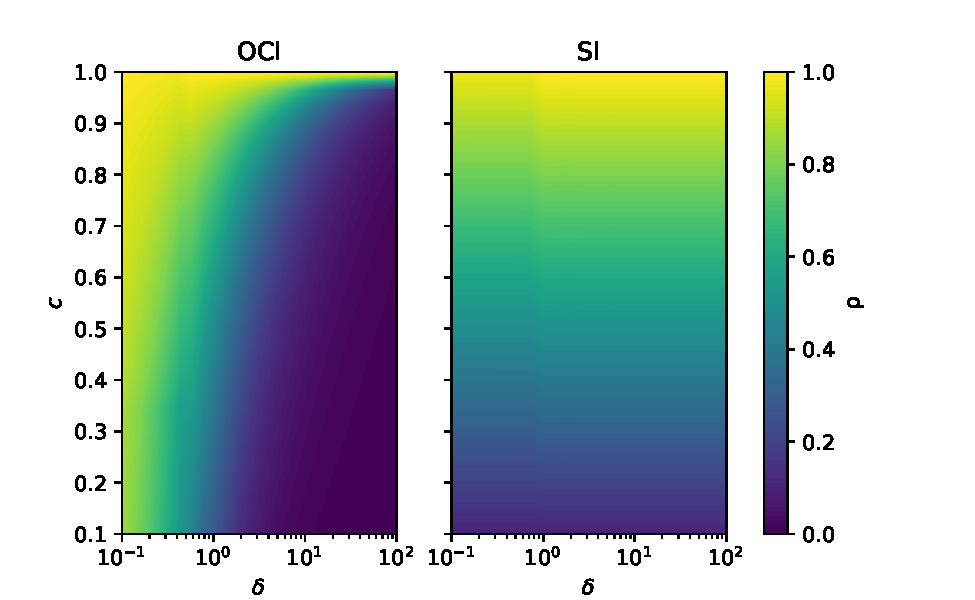
\includegraphics[width=\textwidth]{deterministic/therefore_paper/therefore_figs/ss_specrads.pdf}
    \caption{Spectral radii ($\boldsymbol{\rho}$) of OCI (left) and SI (middle) and the ratio between the two (right), where $\boldsymbol{\Sigma}$ is the total cross section, $\boldsymbol{\Delta x}$ is the cell width, and $\boldsymbol{\Sigma_s}$ is the scattering cross section}
    \label{fig:specrad}
  \end{figure}
Rosa et al. also suggested that future developments in GPU accelerators might overcome this convergence rate decay for problems of interest.
The idea there as that even though more iterations will be required to converge a solution those iterations will be able to be done sufficiently faster (in wall-clock-runtime) to mean a solution is computed faster (again in wall clock runtime) then source iterations.

Other investigations have explored OCI as an acceleration scheme for SI \cite{anistratov_iterative_2015, hoagland_hybrid_2021}. %and a solution to the integral transport matrix method \cite{raffi2108pidotscom} and in the inexact parallel Jacobi scheme.
Previous investigations of OCI as an iterative scheme have been limited to steady state computations.

% potential transient effects in the thin limit 
%When solving discrete ordnance problems for transient systems many codes have implemented Crank-Nicholson or backward Euler time stepping.
%These schemes are non-intrusive often looking like an additional time marching loop around the already implemented transport infrastructure.
Regardless of the time stepping method an OCI iterative algorithm might come with some added befits when used in a transient scheme.
Returning to OCI's spectral radius shown at left in Fig.~\ref{fig:specrad}, since both dimensions are governed by relationships with the cross section of the cell ($\Sigma$), altering that value will impact convergence behavior. 
As the scattering ratio decreases, both iterative algorithms require fewer iterations to converge.
However, the spectral radius of OCI also decreases with increasing optical thickness, \textit{which is an added benefit}.
When solving optically thick and highly scattering problems, small increases in $\Sigma$ may drastically improve the relative performance of OCI in comparison with SI.
%Physically this can be understood as single particles living in single cells for many more iterations.
Time step and cellular optical thickness are inversely proportional to each other, meaning a smaller time step will yield a larger effective total cross section, thus theoretically improving the spectral radius.
This behavior is not expected to happen in source iterations as SI does not directly depend on cellular optical thickness---behaving linearly in that dimension for all but the most thick problems.

\section{Preconditinoers and Synthetic acceleration}

\label{sec:syn_acc}
% acceleration schemes for SI
In order to converge iterative schemes faster many synthetic acceleration techniques have been explored and implemented over the years \cite{adams_fast_2002}.
The most common approach used in conjunction with source iterations is diffusion synthetic acceleration (DSA)\cite{adams_fast_2002}.
The slow convergence of SI in the diffusive limit can be physically understood as there is no linking between angles within an iteration and a diffusive problem is a coupling of angles.
DSA adds a mid-step correction term based off of a cheap to compute diffusion approximation.
%Other synthetic acceleration techniques include Boundary projection acceleration \cite{adams_fast_2002}. %find more

% acceleration schemes for OCI
Previous work has also gone into exploring synthetic acceleration techniques for one cell inversions \cite{ kim_coarse_2000}.
OCI is slow to converge in the thin limit due to the a-synchronicity of the scheme (lagging cell-wise boundary fluxes) \cite{hoagland_hybrid_2021}.
The spectral radius will increase unbounded in the thin limit, regardless of scattering ratio \cite{rosa_cellwise_2013}.
Rosa and Warsa (2009) investigated using transport synthetic acceleration (TSA) as a low order synthetic accelerator, performing a Fourier analysis \cite{tsa2009rosa, tsa_slab2006rosa, tsa_2d2007rosa}.
TSA uses a low order transport sweep with potentially fewer angles and a smaller scattering ratio (often controlled by the user by term $\beta \in [0,1]$) to inform the error correction~\cite{tsa1997gilles}.
In effect, TSA is a less expensive transport sweep that re-couples angles together, which is annoyingly parallel in space and may have significant performance impacts to an OCI scheme.
Rosa and Warsa say as much when they suggest an algorithm where a mesh sweep is only used if convergence hasn't been achieved after a given number of iterations \cite{tsa2009rosa}.
%TSA
%While they suggest future work to implement, no published results of an OCI+TSA scheme.

% gmres
Both SI and OCI are forms of a fixed-point (or Richardson) iteration that use different operator splittings.
In a fixed-point iteration an initial guess of the angular or scalar flux is supplied as a known to the solver which in turn returns an angular or scalar flux (see section \ref{sec:syn_acc}).
This becomes the new guess and this iterative process continues until the relative error between the guess and the output falls below a given tolerance \cite{lewis_computational_1984}.
Krylov methods work by keeping copies of the guess for a given number of previous iterates, compute residuals and ensure the next guess is orthogonal to the previous ones\cite{gmres1996kelley, patton_gmres_2002}.
The generalized minimal residual (GMRES) method specifically, has been shown to make DSA schemes that perform relatively poorly, work well \cite{kylov2004warsa, subspace2004warsa}.


\section{Summary and relation to research questions}

The first publication associated with this work is motivated by the hypothesized additional benefit of OCI in a time dependent code (RQ 3) coupled with the vast improvements in GPU accelerators in the past decade since Rosa et al. \cite{rosa_cellwise_2013} conducted their investigations (RQ 1 and 2).
A rough draft of this first publication is included in Appendix \ref{app:therefore}.
I plan to submit this work before the new year.
The next publication will be an exploration of a synthetic acceleration algorithm to converge OCI in the thin limit (RQ 4).
%Furthermore, as previously mentioned, source iterations are often implemented in production accompanied by some kind of synthetic-acceleration scheme or other preconditioner to converge it's slowest converging mode (the diffusive limit).
%OCI has never been implemented with a prevonditon

To recast the neutron radiation transport equation (Eq.~\eqref{eq:fullNTE}) into a form solvable on digital computers, continuous functions of space, time, angle, and energy must be discretized.
An iterative scheme is also required for memory and computationally efficient calculations.
In this section I describe the discretizations and their assumptions for the 1D, time-dependent, multi-group solver discussed within this work.
I will also describe the two fixed-point iterative schemes that I implement and discuss gaps in previous work of deterministic iterative solvers.
My work with deterministic schemes can be separated into two categories:
\begin{enumerate}
    \item How to use software engineering libraries to implement work more efficiently (RQ 1); and
    \item Novel methods to converge the solution faster on modern hardware
    \begin{enumerate}
        \item A space-parallel iterative scheme on modern HPC GPUs (RQ2);
        \item How transient behavior impacts convergence of a space-parallel iterative scheme (RQ3); and
        \item How to accelerate the space-parallel iterative scheme to converge faster (RQ4)
    \end{enumerate}
\end{enumerate}


\newpage
\renewcommand{\TheTitle}{One-Cell Inversion for Solving Higher-Order Time-Dependent Radiation Transport on GPUs}
\renewcommand{\TheAuthors}{Joanna Piper Morgan,
  Ilham Variansyah,
  Todd S. Palmer, and
  Kyle E. Niemeyer}

\renewcommand{\TheAddress}{
    \textit{Nuclear Science and Engineering} \\
    Vol.~VOLUME, PAGES, YEAR. \\
    \doi{10.1016/xxxx}
}

\PaperHeader{\TheTitle}{\TheAuthors}{\TheAddress}

\chapter{\TheTitle}
\label{chapter:therefore_paper}

\epigraphhead[10]{\singlespacing
    \epigraph{
        The stupidest person on God's green earth is the 2nd lieutenant in the US army. The only person who might rival that; would be an engineer right out of school---dont be so fucking stupid
    }
    {Evan H Morgan (my grandfather)}
}



\section*{Abstract}
To find deterministic solutions to the transient discrete-ordinates neutron-transport equation, source iterations (SI) are typically used to lag the scattering (and fission) source terms from subsequent iterations.
For Cartesian geometries in one dimension, SI is parallel over the number of angles but not spatial cells; this is a disadvantage for many-core compute architectures like graphics processing units.
One-cell inversion (OCI) is a class of alternative iterative methods that allow space-parallel radiation transport on heterogeneous compute architectures.
For OCI, previous studies have shown that, in steady-state computations, spectral radius tends to unity when cells are optically thin regardless of the scattering ratio.
In this work, we analyze how the convergence rate of an OCI scheme behaves when used for time-dependent neutron transport computations.
We derive a second-order space-time discretization method from the simple corner balance and multiple balance time discretization schemes and show via Fourier analysis that it is unconditionally stable through time.
Then, we derive and numerically solve the Fourier systems for both OCI and SI splittings of our discretization, showing that small mean-free times improve the spectral radius of OCI more than SI, and that spectral radius for OCI tends to zero as mean free time gets smaller.
We extend both solvers to be energy dependent (using the multi-group assumption) and implement on an AMD MI250X using vendor-supplied batched LAPACK solvers.
Smaller time steps improve the relative performance of OCI over SI, and, even when OCI requires more iterations to converge a problem, those iterations can be done much faster on a GPU.
This leads to OCI performing better overall than SI on GPUs.

\section{Introduction}

% more general intro problem applications -> Sn transport
Simulating transient particle transport is often required when computing the solution to a number of multi-physics problems, including burst criticality experiments, fission reactor accidents, and other highly dynamic systems.
% Problems to solve and Sn transport
Finding deterministic solutions to the transient neutron transport equation requires some method of treating the contribution of scattering described by an integral.
This is either done by taking moments of the neutron transport equation and making a closure assumption, or by using quadrature to discretize the integral over angle.
The latter is called the method of discrete ordinates (or S$_N$ method, where $N$ is the number of angles in a one-dimensional quadrature set) that forms a coupled set of simultaneous PDEs, with one for every direction in a given quadrature set.
The contribution to the scattering source can then be computed using a sum over angles of weights times quantities of interest.
Typically, iterative schemes from operator splitting are used to treat the scattering (and fission) source terms that arise in this coupled set of partial differential equations \cite{lewis_computational_1984}.

% State of the art of transport solvers on CPUs and GPUs warsaw paper
Source iteration (SI), often accompanied by preconditioners or synthetic accelerators, is a common iteration approach: the contribution to the solution from the scattering source lags, while the angular flux is solved in every ordinate direction via ``sweeps'' through the spatial domain~\cite{adams_subcell_1997}.
SI sweeps in Cartesian geometries readily parallelize over the number of angles.
While any parallelization improves performance, a scheme that is embarrassingly parallel over the dimension with the greatest number of degrees of freedom---space---would be advantageous, especially on vectorized hardware \cite{rosa_cellwise_2013, hoagland_hybrid_2021}.
In slab geometry, SI sweeps can be parallelized in angle and energy groups (via Jacobi iteration), but are serial in space as information about the angular flux incident on edges of each cell is required before the computation can proceed.

In higher spatial dimensions, many S$_N$ production codes that implement SI use a wavefront marching parallel algorithm known as a Koch--Baker--Alcouffe scheme \cite{baker_kba_2017}, also called ``full parallel sweeps.''
This algorithm begins a sweep in a spatial location where all cell dependencies are known from boundary information (e.g., a corner).
From there, on a hypothetical orthogonal 2D spatial grid the two nearest neighbor cells are computed independently in parallel; the next step would be across four cells.
This diagonally expanding wavefront continues to march and can compute quantities of interest in parallel for as many cells that lie on the diagonal sweep step.
These sweeps are done on structured or unstructured finite element or finite volume spatial discretizations with backward Euler or Crank--Nicholson time stepping iterations.
Source iteration is often solved with preconditioned fixed-point (Richardson) or Krylov sub-space methods (e.g., GMRES) \cite{adams_fast_2002}.

An alternative to SI is one-cell inversion (OCI), a class of operator splitting that computes all angular fluxes in all ordinates within a cell in a single linear algebra solve, assuming that the angular fluxes incident on the surfaces of the cell are known from a previous iteration \cite{kang2000oci}.
OCI methods allow parallelizing over the number of cells, as each cell is solved independently in parallel.
OCI iterations can take the form of a cell-wise block-Jacobi, cell-wise block-Gauss--Seidel, or cell-wise red-black iteration depending on the order in which cells are inverted \cite{man1994parallel}.
Like SI, OCI iterations can be fixed-point (Richardson) or non-stationary schemes like GMRES \cite{kylov2004warsa}, with or without preconditioners (including diffusion synthetic acceleration \cite{kang2000oci}) on structured and unstructured meshes.
Parallel block Jacobi and parallel block Gauss--Seidel iterations may also be used for domain decomposition with transport sweeps within subdomains \cite{qiao_improved_2021}.
In fact, OCI methods can be thought of as a cellular decomposed version of these schemes.

\cite{rosa_cellwise_2013} previously studied cell-wise block Jacobi and cell-wise block Gauss--Seidel as a potentially superior iterative scheme over SI preconditioned with diffusion synthetic acceleration on vectorized architectures.
They hypothesized that OCI schemes might outperform an SI preconditioned with diffusion synthetic acceleration and using full-parallel sweeps in terms of wall-clock runtime, because of OCI's parallelism over the dominant domain (space), the ability to take advantage of vendor-supplied LAPACK type libraries, high arithmetic-intensity operations present in an OCI algorithm, and superior spectral properties in the thick limit.
Rosa et al.\ conducted Fourier analysis for and implemented OCI in a 2D, multi-group, steady-state code using bilinear discontinuous finite elements to discretize space.
They paired this with either a cell-wise block Jacobi and cell-wise block Gauss--Seidel iteration algorithm.
The study was conducted on the (then) state-of-the-art RoadRunner supercomputer and took advantage of its 64-bit PowerXCell vectorized accelerator.
However, the acceleration per iteration in the block Gauss--Seidel OCI implementation did not make up for the degradation of convergence that OCI methods incur in the thin limit.

OCI can require more iterations to converge to a solution for some problems, since no information exchanges between cells within an iteration.
Specifically, as cellular optical thickness decreases, OCI's relative performance degrades.
Spectral radius ($\rho$) of OCI tends to unity in the thin cell limit---regardless of the scattering ratio---due to the algorithm decoupling cells from one another (i.e., asynchronicity) \cite{rosa_cellwise_2013, hoagland_hybrid_2021, man1994parallel}. 
Figure~\ref{fig:ss-sepcrad} illustrates this behavior, showing the spectral radii of the two iteration schemes as a function of cellular optical thickness, $\delta$ (in mean free paths), and the scattering ratio, $c$.
We compute these values using Fourier analysis of an infinite medium slab problem using S$_{8}$ angular quadrature for block Jacobi OCI and unpreconditioned SI iterative schemes\footnote{Gauss--Legendre quadrature is used in all presented work.}.
The spectral radius of SI depends strongly on the scattering ratio but is independent of $\delta$ for the homogeneous infinite-medium problem. 
Compared to SI, OCI rapidly converges in thicker cells, even in highly scattering problems except for scattering ratios closest to one.

\begin{figure}
    \centering
    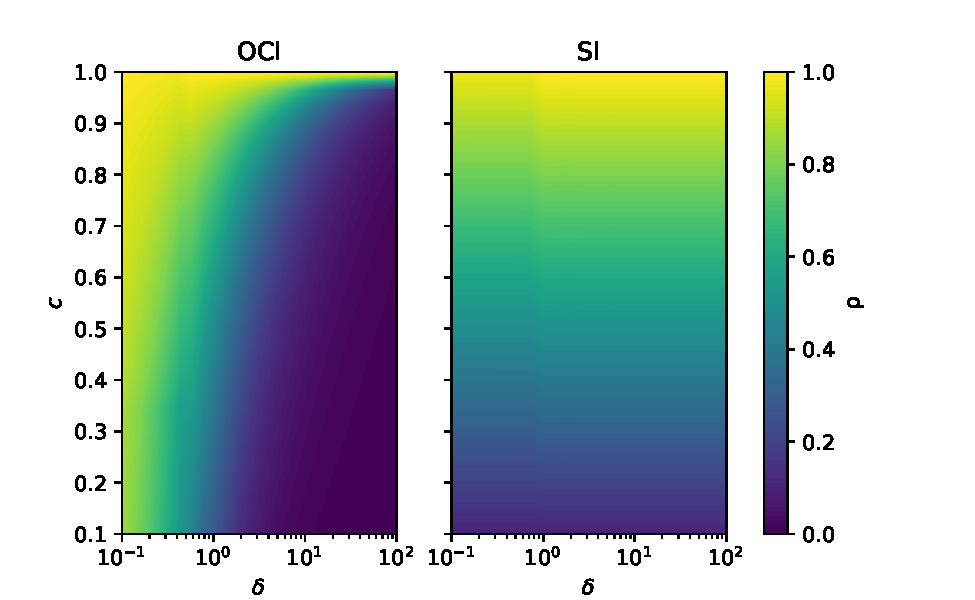
\includegraphics[width=\textwidth]{deterministic/therefore_paper/therefore_figs/ss_specrads.pdf}
    \caption{Spectral radii (${\rho}$) of steady-state OCI (left) and SI (right), where $c$ is the scattering ratio and ${\delta}$ is the cellular optical thickness in mean free paths from Fourier analysis in S$_8$.}
    \label{fig:ss-sepcrad}
\end{figure}

Others have explored OCI as an acceleration scheme for SI \cite{ hoagland_hybrid_2021}, a component of a multi-grid solver \cite{man1995multigrid1, man1996multigrid2}, and a solution to the integral transport matrix method \cite{raffi2108pidotscom}.
However, previous investigations of OCI are limited to steady-state computations.

When employing implicit time-differencing schemes (e.g., Crank--Nicholson, backward Euler), each time step involves the solution of a steady-state transport problem with an effective total cross section that includes a time absorption term, proportional to $1/(v \Delta t)$, where $\Delta t$ is time step size and $v$ is radiation speed.
Returning to Fig.~\ref{fig:ss-sepcrad}, the macroscopic total cross section ($\Sigma$) influences both the optical thickness of the cell ($\delta$) and the scattering ratio ($c$), so increasing or decreasing $\Sigma$ will impact convergence behavior.
Spectral radius for both iterative methods decreases as the scattering ratio decreases, but \textit{the spectral radius of OCI also decreases with increasing optical thickness}, which in turn depends on $\Sigma$.
When solving optically thin and highly scattering problems, small increases to $\Sigma$ (and for time-dependent problems, decreases in $\Delta t$ or $v$) may drastically improve the relative performance of OCI compared to SI.
This hypothesis motivates our work, along with evaluating cell-wise algorithms on modern GPU accelerators and exploring higher-order space-time discretization schemes.

We previously derived a second-order space (simple corner balance), and time discretization (multiple balance) scheme for block Jacobi OCI (which we will call simply OCI in the remainder of this work) \cite{morgan2023oci}.
We previously showed that when there are more spatial degrees of freedom than in angle, a GPU implementation of OCI will outperform a similarly implemented version of SI in wall clock runtime, in all but the highest scattering problems, for quadrature orders between \num{16} and \num{64} for mono-energetic 1D problems. 

Some derivations from our previous work are included here (Section~\ref{sec:methods-derv}), because we extend it with a Fourier analysis of the discretization scheme through time to ensure it remains unconditionally stable.
We also perform a Fourier analysis on a single time step of OCI and SI to study convergence behaviors in various limits under transient conditions.
Furthermore we extend our derivations to multi-group problems and implement both OCI and SI on an AMD MI250X GPU using vendor-supplied libraries to confirm Fourier results and analyze performance.

\section{Methods}

In this section, we derive the discretized equations for the initial and boundary value problem and describe the OCI iteration.
We have chosen to implement robust second-order discretization methods: simple corner balance  \cite{adams_subcell_1997} in space and multiple balance \cite{variansyah_robust_2021} in time.
By coupling these higher accuracy schemes with an efficient iterative method, we hope to optimize the ratio of compute work to communication work to better suit the numerical method for GPUs.
To confirm that multiple balance time discretization remains unconditionally stable with simple corner balance, we conduct Fourier analysis for a non-scattering model problem.
Then, we derive the Fourier system for a single time step of simple corner balance + multiple balance discretization using both OCI and SI operator splitting to study the convergence rate.
Finally, we present systems for multi-group transport.

\subsection{Derivation of space and time discretization for one-cell inversion}
\label{sec:methods-derv}
We begin with the time-dependent, isotropic scattering slab geometry, S$_N$ transport equations with an isotropic source.
\begin{multline}
    \label{eq:sn_nte}
    \frac{1}{v} \frac{\partial \psi_{m}(x,t)}{\partial t} + \mu_m \frac{\partial \psi_{m}(x,t)}{\partial x} + \Sigma(x) \psi_{m}(x,t) 
     = \frac{1}{2} \left( \Sigma_{s}(x) \sum\limits_{n=1}^N w_n \psi_{n}(x,t) + Q(x,t) \right) \;, \\
    \qquad \qquad m=1, \ldots, N \;, \qquad t > 0 \;, \qquad x \in [0,X]
\end{multline}
where $\psi$ is the angular flux, $t$ is time, $x$ is location, $v$ is speed, $\Sigma$ is the macroscopic total cross-section, $\Sigma_s$ is the macroscopic scattering cross-section, $w_m$ is angular quadrature weight, $\mu_m$ is the angular quadrature ordinate, $m$ is the quadrature index, $N$ is the quadrature order, and $Q$ is the isotropic material source.
The initial and boundary conditions are prescribed angular flux distributions:
\begin{equation*}
    \psi_{m}(x,0) = \psi_{init,m}(x), \qquad m=1 \ldots N \;,
\end{equation*}
\begin{equation*}
    \psi_{m}(0,t) = \psi_{inc,m}^+(t), \qquad \mu_m >0 \;,
\end{equation*}
\begin{equation*}
    \psi_{m}(X,t) = \psi_{inc,m}^-(t), \qquad \mu_m <0 \;.
\end{equation*}
We discretize these equations in time using multiple balance~\cite{variansyah_robust_2021}, which solves two coupled sets of equations. 
First is a backward Euler step (transport equation integrated over a time step):
\begin{subequations}
\begin{multline}
\frac{1}{v} \left( \frac{\psi_{m,k+1/2}(x) - \psi_{m,k-1/2}(x)}{\Delta t} \right) + \mu_m \frac{\partial \psi_{m,k}(x)}{\partial x} + \Sigma(x) \psi_{m,k}(x) \\
= \frac{1}{2} \left(  \Sigma_{s}(x) \sum\limits_{n=1}^N w_n \psi_{n,k}(x) + Q_{k}(x) \right) \;,
\end{multline}
and the second is a balance like auxiliary equation from the multiple balance principle:
\begin{multline}
\frac{1}{v} \frac{\psi_{m,k+1/2}(x) - \psi_{m,k}(x)}{\Delta t/2} + \mu_m \frac{\partial \psi_{m,k+1/2}(x)}{\partial x} + \Sigma(x) \psi_{m,k+1/2}(x) \\
= \frac{1}{2} \left( \Sigma_{s}(x) \sum\limits_{n=1}^N w_n \psi_{n,k+1/2}(x) + Q_{ k+1/2}(x) \right) \;,
\end{multline}
\end{subequations}
where $\Delta t$ is the time step size, $k$ indicates time-average quantities, and $k\pm1/2$ indicates time-edge quantities.
Then, we discretize in space using simple corner balance, which involves a spatial integration over the right and left halves of a spatial cell:
\begin{subequations}
\label{eq:scb-mb}
\begin{multline}
\label{eq:scb-mb-a}
\frac{\Delta x_j}{2} \frac{1}{v} \left( \frac{\psi_{m,k+1/2,j,L} - \psi_{m,k-1/2,j,L}}{\Delta t} \right)
 + \mu_m \left[ \frac{\left( \psi_{m,k,j,L} + \psi_{m,k,j,R} \right)}{2}  - \psi_{m,k,j-1/2} \right] \\
+ \frac{\Delta x_j}{2} \Sigma_{j} \psi_{m,k,j,L} 
= \frac{\Delta x_j}{2} \frac{1}{2} \left( \Sigma_{s,j} \sum\limits_{n=1}^N w_n \psi_{n,k,j,L} + Q_{k,j,L} \right) \;,
\end{multline}  
\begin{multline}
\label{eq:scb-mb-b}
\frac{\Delta x_j}{2} \frac{1}{v} \left( \frac{\psi_{m,k+1/2,j,R} - \psi_{m,k-1/2,j,R}}{\Delta t} \right) +
\mu_m \left[ \psi_{m,k,j+1/2} - \frac{\left( \psi_{m,k,j,L} + \psi_{m,k,j,R} \right)}{2}   \right] \\
+ \frac{\Delta x_j}{2} \Sigma_{j} \psi_{m,k,j,R} = \frac{\Delta x_j}{2} \frac{1}{2} \left( \Sigma_{s,j} \sum\limits_{n=1}^N w_n \psi_{n,k,j,R} + Q_{k,j,R} \right) \;,
\end{multline}  
\begin{multline}
\label{eq:scb-mb-c}
\frac{\Delta x_j}{2} \frac{1}{v} \left( \frac{\psi_{m,k+1/2,j,L} - \psi_{m,k,j,L}}{\Delta t/2} \right) \\
+ \mu_m \left[ \frac{\left( \psi_{m,k+1/2,j,L} + \psi_{m,k+1/2,j,R} \right)}{2}  - \psi_{m,k+1/2,j-1/2} \right]
+ \frac{\Delta x_j}{2} \Sigma_{j} \psi_{m,k+1/2,j,L} \\
= \frac{\Delta x_j}{2} \frac{1}{2} \left( \Sigma_{s,j} \sum\limits_{n=1}^N w_n \psi_{n,k+1/2,j,L} + Q_{k+1/2,j,L} \right) \;,
\end{multline}    
\begin{multline}
\label{eq:scb-mb-d}
\frac{\Delta x_j}{2} \frac{1}{v} \left( \frac{\psi_{m,k+1/2,j,R} - \psi_{m,k,j,R}}{\Delta t/2} \right) + \\
\mu_m \left[ \psi_{m,k+1/2,j+1/2} - \frac{\left( \psi_{m,k+1/2,j,L} + \psi_{m,k+1/2,j,R} \right)}{2}   \right]
+ \frac{\Delta x_j}{2} \Sigma_{j} \psi_{m,k+1/2,j,R} \\
= \frac{\Delta x_j}{2} \frac{1}{2} \left( \Sigma_{s,j} \sum\limits_{n=1}^N w_n \psi_{n,k+1/2,j,R} + Q_{k+1/2,j,R} \right) \;,
\end{multline} 
\end{subequations}
where $\Delta x$ is the cell width, $j$ is the spatial cell index, $L/R$ is the left or right half cell, respectively.
These equations contain the first of the two simple spatial closures---the angular flux at the cell midpoint is a simple average of the two half-cell average quantities:
\begin{subequations}
\begin{equation}
  \psi_{m,k}(x_j) =  \frac{\left( \psi_{m,k,j,L} + \psi_{m,k,j,R} \right)}{2} \;,
\end{equation}
\begin{equation}
  \psi_{m,k+1/2}(x_j) =  \frac{\left( \psi_{m,k+1/2,j,L} + \psi_{m,k+1/2,j,R} \right)}{2} \;.
\end{equation}
\end{subequations}
The second closure is an \textit{upstream} prescription for the cell-edge angular flux:
\begin{subequations}
\begin{equation}
  \psi_{m,k,j+1/2} =
  \begin{cases}
  \psi_{m,k,j,R}, & \mu_m > 0, \\
  \psi_{m,k,j+1,L}, & \mu_m < 0 \;,
  \end{cases}
\end{equation}
\begin{equation}
  \psi_{m,k+1/2,j+1/2} =
  \begin{cases}
  \psi_{m,k+1/2,j,R}, & \mu_m > 0, \\
  \psi_{m,k+1/2,j+1,L}, & \mu_m < 0 \;.
  \end{cases}
\end{equation}
\end{subequations}
Figure~\ref{fig:stencil} shows the stencil location for angular flux and source terms. 
\begin{figure}
    \centering
    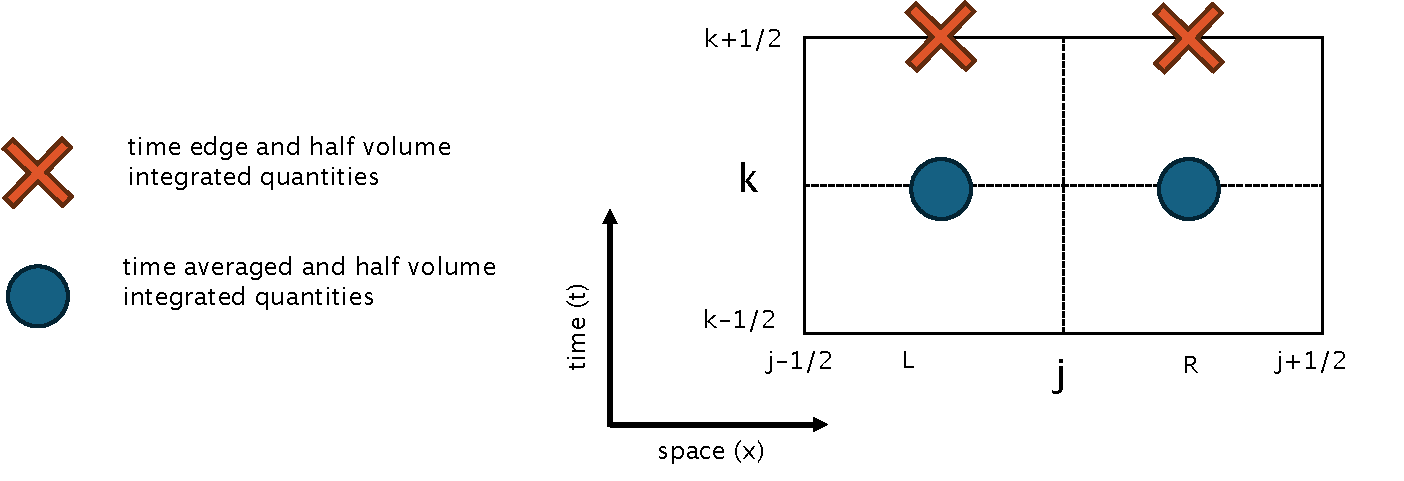
\includegraphics[width=\textwidth]{deterministic/therefore_paper/therefore_figs/stencil.pdf}
    \caption{Discretization stencil for simple corner balance, multiple balance time discretization}
    \label{fig:stencil}
\end{figure}

Solving Eqs.~\eqref{eq:scb-mb} iteratively requires operator splitting.
Unknown values (from the current iteration, noted by $(l+1)$) are moved to the left-hand side to form a large system of linear equations.
In SI, the scalar flux in the scattering source is evaluated at the previous iteration $(l)$, decoupling angles and coupling space.
OCI allows the fluxes incident to the cell---defined by upstream closures---to lag, thus decoupling cells from one another within an iteration.

In OCI, the scattering source is subtracted to the left-hand side and  prior iteration values are employed for all information incident on cell $j$ (moved to the right-hand side).
This means that all $4N$ angular fluxes ($N$ angles at $L$ and $R$, $k$ and $k+1/2$) are computed simultaneously in cell $j$.
This yields a linear system for each cell $j$:
\begin{equation}
    \label{eq:oci}
    \left( \bm{L}_{c,j} - \bm{S}_j \right) \Psi_j^{(l+1)} = -\textbf{L}_{b,j} \Psi_j^{(l)} + \textbf{Q} \;, 
\end{equation}
where $l$ is the iteration index.
The right-hand side can be combined into a known vector
\begin{equation}
     \left( \bm{L}_{c,j} - \bm{S}_j \right) \Psi_j^{(l+1)}  = \bm{b}_j \; ,
\end{equation}
where $\bm{L}_{c,j}$ and $\bm{S}_j$ are both of size $4N\times4N$ and likewise $\bm{b}_j$ is a vector of length $4N$.
\newcommand{\lcmj}[1]{\begin{bmatrix} \bm{L}_{c,j,#1} \end{bmatrix} }
\newcommand{\zeros}{\begin{bmatrix} 0 \end{bmatrix} }
The within-cell operator is
\begin{subequations}
\begin{equation}
    \label{eq:Aja}
    \bm{L}_{c,j} = \begin{bmatrix}
        \lcmj{1} &  &  &  &  \\
          & \ddots  &  &  & \\
          &  & \lcmj{m} &  & \\
          &  &  & \ddots &  \\
          &  &  &  & \lcmj{N}
    \end{bmatrix} \;,
\end{equation}
with zeros elsewhere, where
\begin{equation} \bm{L}_{c,j,m} =
    \label{eq:Aj}
    \begin{bmatrix}
    \frac{|\mu_m| + \Delta x_j \Sigma_{j} }{2}  & \frac{\mu_m}{2} & \frac{\Delta x_j}{2 v \Delta t} & 0 \\
    - \frac{\mu_m}{2} & \frac{|\mu_m| +  \Delta x_j \Sigma_{j,g} }{2} & 0 & \frac{\Delta x_j}{2 v \Delta t} \\
    -\frac{\Delta x_j}{v \Delta t}  & 0 & \frac{\Delta x_j}{v \Delta t} + \frac{|\mu_m| + \Delta x_j \Sigma_{j,g} }{2}  & \frac{\mu_m}{2}  \\
    0 &  -\frac{\Delta x_j}{v \Delta t}  &  - \frac{\mu_m}{2} & \frac{\Delta x_j}{v \Delta t}+ \frac{|\mu_m| + \Delta x_j \Sigma_{j,g}}{2}  \\
    \end{bmatrix} \; .
\end{equation}
\end{subequations}
The right-hand side is
\begin{subequations}
\label{eq:rhs_sg}
\begin{equation}
    \bm{b}_j =  \left[
    \bm{b}_{j,1} \; \bm{b}_{j,2} \; \cdots \; \bm{b}_{j,N} \right]^{T} \;.
\end{equation}
As the linear system in each cell contains contributions from all angles (both positive and negative) $b_{j,m}$ is given by
\begin{equation} 
    \bm{b}_{j,m} = 
    \begin{cases}
        \bm{b}_{j,m}^+ & \mu_m>0 \\
        \bm{b}_{j,m}^- & \mu_m<0 \\
    \end{cases} \;,
\end{equation}
where
\begin{equation}
     \bm{b}_{j,m}^+ = \begin{bmatrix}
     \frac{\Delta x_j}{4} Q_{k,j,L} + \frac{\Delta x_j}{2 v \Delta t} \psi_{m,k-1/2,j,L} + \mu_m \psi^{(l)}_{m,k,j-1,R} \\
     \frac{\Delta x_j}{4}Q_{k,j,R} + \frac{\Delta x_j}{2 v \Delta t} \psi_{m,k-1/2,j,R} \\
     \frac{\Delta x_j}{4}Q_{k+1/2,j,L} + \mu_m \psi^{(l)}_{m,k+1/2,j-1,R} \\
     \frac{\Delta x_j}{4} Q_{k+1/2,j,R} 
    \end{bmatrix} \;,
\end{equation}
and
\begin{equation}
    \bm{b}_{j,m}^- = \begin{bmatrix}
    \frac{\Delta x_j}{4}  Q_{k,j,L} + \frac{\Delta x_j}{2 v \Delta t} \psi_{m,k-1/2,j,L}  \\
    \frac{\Delta x_j}{4}  Q_{k,j,R} + \frac{\Delta x_j}{2 v \Delta t} \psi_{m,k-1/2,j,R} - \mu_m \psi^{(l)}_{m,k,j+1,L}  \\
    \frac{\Delta x_j}{4}  Q_{k+1/2,j,L}  \\
    \frac{\Delta x_j}{4}  Q_{k+1/2,j,R} - \mu_m \psi^{(l)}_{m,k+1/2,j+1,L}
    \end{bmatrix} \;.
\end{equation}
\end{subequations}
The elements of the ${S_j}$ matrix are defined by
\begin{equation}
    \label{eq:scatter}
   [\mathbf{S}_j]_{k,l} = \begin{cases}
			\frac{\Delta x_j \Sigma_{s,j}}{4}w_{\frac{|(r-s)|}{3}}, & \text{if $\mod{\frac{(r-s)}{3} =0}$}\\
            0, & \text{otherwise}
		 \end{cases} \; ,
%  \frac{\Delta x_j \Sigma_{s,j}}{4} w_n \; l=r k=s
\end{equation}
where $w$ are the angular quadrature weights, and $r$ and $s$ are the rows and columns of the scattering matrix, respectively.
Finally,
\begin{subequations}
\label{eq:x_vec}
\begin{equation}
\Psi^{(l+1)}_j =  \begin{bmatrix}
    \bm{\psi}_{j,1}^{(l+1)}, \;
    \bm{\psi}_{j,2}^{(l+1)}, \;
    \cdots \;
    \bm{\psi}_{j,N}^{(l+1)}
    \end{bmatrix} ^{T} \; ,
\end{equation}
where
\begin{equation} 
\bm{\psi}_{j,n}^{(l+1)} = \begin{bmatrix}
    \psi_{n,k,j,L}^{(l+1)}, \;
    \psi_{n,k,j,R}^{(l+1)}, \;
    \psi_{n,k+1/2,j,L}^{(l+1)}, \;
    \psi_{n,k+1/2,j,R}^{(l+1)}
    \end{bmatrix}^{T} \;.
\end{equation}
\end{subequations}
One-cell inversion iterations continue until
\begin{equation}
    ||\Psi^{(l+1)}-\Psi^{(l)}||_{2} < \epsilon(1-\rho_e) \; ,
\end{equation}
where $\epsilon$ is the convergence tolerance and
\begin{equation}
    \rho_e = \frac{||\Psi^{(l+1)}-\Psi^{(l)}||_{2}}{||\Psi^{(l)}-\Psi^{(l-1)}||_{2}} \; ,
\end{equation}
is an empirical estimation of the spectral radius computed at every iteration of a transport solve.
After convergence, the time-step counter increments and the time-step process can be repeated.

Generally, Jacobi and Gauss--Seidel iterations converge faster when a system is more diagonally dominant \cite{isaacson_numerical_1966, golub_matrix_1983}.
Equation~\eqref{eq:Aj} contains ($ \delta/2 = \Delta x\Sigma/2 $) on the diagonals.
So in the thin limit (when $\delta\rightarrow 0$) the system becomes overall less diagonally dominant and converges more slowly.
However Equation~\eqref{eq:Aj} also involves $\Delta x/(v\Delta t)$ terms in elements (3,3) and (4,4).
Thus, a smaller time step will cause the system to become more diagonally dominant.
We provide a similar description of simple corner balance and multiple balance time discretization for an unpreconditioned source iteration \cite{morgan2023oci}.

\subsection{Fourier analysis: time-stepping scheme}

To ensure that the combination of higher-order discretization schemes remains an unconditionally stable time-marching method, we perform Fourier analysis (also known as Von Neumann stability analysis)~\cite{leveque2007finite}.
A time marching scheme
\begin{equation}
    \Psi_{k+1/2} = \bm{K} \Psi_{k-1/2} \;,
\end{equation}
where $\bm{K}$ is the time iteration matrix, is unconditionally stable when the Von Neumann stability condition is met:
\begin{equation}
    \sup(|\lambda_{K}|) \leq 1 \;,
    \label{eq:unconstab}
\end{equation}
where $\lambda_{K}$ are all the eigenvalues of $\bm{K}$ \cite{golub_matrix_1983, isaacson_numerical_1966}.
$\bm{K}$ can be derived for a given model problem.
We consider a model problem consisting of a homogeneous infinite medium with no scattering to derive the eigenfunction of the time-dependent multiple balance, simple corner balance discretization scheme.
Since this problem has no scattering, each angle can be solved independently of every other angle, and no operator splitting is required.
We first start by describing the absolute error of the angular flux at time step $(k+1/2)$:
\begin{equation}
    \mathbf{f}_{k+1/2} = \Psi_{\text{exact}} - \Psi_{k+1/2} \;.
\end{equation}
We then assume that each unknown representing the error on our discretization stencil is expanded in a series of temporal Fourier modes, where each mode has a coefficient ($a$, $b$, $c$, or $d$), an amplitude ($\lambda$), and a shape function ($e^{i\omega x}$).
We can then define a Fourier ansatz for the error propagated through a time step:
\begin{subequations}
\begin{align}
    f_{k+1/2,j,L} &= \lambda^{k+1}a e^{i\omega j} \; ,
    &
    f_{k+1/2,j,R} &= \lambda^{k+1}b e^{i\omega j} \; ,
\end{align}
\begin{align}
    f_{k,j,L} &= \lambda^{k}c e^{i\omega j} \; ,
    &
    f_{k,j,R} &= \lambda^{k}d e^{i\omega j} \; ,
\end{align}
\begin{align}
    f_{k-1/2,j,L} &= \lambda^{k}a e^{i\omega j} \; ,
    &
    f_{k-1/2,j,R} &= \lambda^{k}b e^{i\omega j} \; ,
\end{align}
\end{subequations}
where $k$ is the time step, $i=\sqrt{-1}$, $\lambda$ is the eigenvalue, $\omega$ is the wave number, and $j$ is cell index. 
Substituting our ansatz into the error form of Eqs.~\eqref{eq:scb-mb} and assuming $\mu>0$, we simplify to form
\begin{subequations}
\begin{equation}
    \label{eq:eig1}
    \frac{\Delta x}{2} \frac{1}{v \Delta t} (\lambda a- a) + \mu \left(\frac{c+d}{2} - d e ^{-i\omega} \right) + \frac{\Sigma\Delta x }{2}c = 0 \; ,
\end{equation}
\begin{equation}
\label{eq:eig2}
    \frac{\Delta x}{2} \frac{1}{v \Delta t} (\lambda b - b) + \mu \left( ce^{i\omega} - \frac{c+d}{2} \right) + \frac{\Sigma\Delta x }{2}d = 0 \; ,
\end{equation}
\begin{equation}
\label{eq:eig3}
    \frac{\Delta x}{2} \frac{2}{v \Delta t} (\lambda a - c) + \lambda\mu \left( \frac{a+b}{2} - b e^{-i\omega} \right) + \frac{\Sigma\Delta x }{2}a \lambda = 0 \; ,
\end{equation}
\begin{equation}
\label{eq:eig4}
    \frac{\Delta x}{2} \frac{2}{v \Delta t} (\lambda b - d) + \lambda\mu \left( d e^{i\omega} + \frac{c+d}{2} \right) + \frac{\Sigma\Delta x}{2} b\lambda = 0 \;.
\end{equation}
\end{subequations}
Next, we combine Eq.~\eqref{eq:eig1} into \eqref{eq:eig2}:
\begin{equation}
    \label{eq:f_a-1}
    \begin{bmatrix}
        c\\d
    \end{bmatrix}
    = \bm{K_{+}}^{-1} \frac{\Delta x}{2}\frac{1}{v\Delta t}(1-\lambda)
    \begin{bmatrix}
        a\\b
    \end{bmatrix} \;,
\end{equation}
where
\begin{equation}
    {\bm{K_{+}}} = 
    \begin{bmatrix}
    \frac{\mu}{2}+\frac{\Sigma \Delta x}{2} & \mu (\frac{1}{2} - e^{-i\omega}) \\
    -\frac{\mu}{2} & \frac{\mu}{2}+\frac{\Sigma \Delta x}{2}
    \end{bmatrix} \;.
\end{equation}
Then, doing the same with Eq.~\eqref{eq:eig3} into \eqref{eq:eig4}:
\begin{equation}
    \label{eq:f_a-2}
    \lambda \left( \bm{K_{+}} + \frac{\Delta x}{v \Delta t} \bm{I} \right)  \begin{bmatrix}
        a \\ b
    \end{bmatrix} = \frac{\Delta x}{v\Delta t} \begin{bmatrix}
        c \\ d
\end{bmatrix} \; ,
\end{equation}
where $\bm{I}$ is the identity matrix. Combining Eq.~\eqref{eq:f_a-1} into \eqref{eq:f_a-2} gives
\begin{equation}
    \lambda
    \begin{bmatrix}
        a \\b
    \end{bmatrix}
    = \left[ \bm{K_{+}} + \frac{\Delta x}{v\Delta t} \bm{I} + \gamma\bm{K_{+}}^{-1} \right]^{-1} \gamma \bm{K_{+}}^{-1}
    \begin{bmatrix}
        a \\ b
    \end{bmatrix} \; ,
\end{equation}
where $\gamma = \frac{\Delta x}{v\Delta t}  \frac{\Delta x}{2v\Delta t}$.
This can then be more appropriately posed as an eigenfunction:
\begin{equation}
    \lambda_K
    \bm{a}
    = \bm{K} \bm{a}\;,
\end{equation}
where
\begin{equation}
    \bm{K} = \gamma \left( \bm{K_{+}}\bm{K_{+}} + \frac{\Delta x}{v \Delta t}\bm{K_{+}} + \gamma \bm{I}\right)^{-1}
\end{equation}
and the eigenvector is
\begin{equation}
    \bf{a} = \begin{bmatrix}
        a, & b
    \end{bmatrix} ^T \;.
\end{equation}
The analysis is similar for $\mu<0$ only with
\begin{equation}
    \bm{K_{-}} = \begin{bmatrix}
        -\frac{\mu}{2} + \frac{\Sigma\Delta x}{2} & \frac{\mu}{2} \\
        \mu \left ( e^{i\omega} - \frac{1}{2} \right) & -\frac{\mu}{2} + \frac{\Sigma\Delta x}{2} 
    \end{bmatrix} \;.
\end{equation}

This system can be numerically solved after making discrete selections of $\mu \in [-1, 1]$ and $\omega \in (0,2\pi]$ at a point in the perameter space ($\Delta x$, $\Delta t$, $v$, $\Sigma$) with \texttt{numpy.max(numpy.abs(numpy.linalg.\\eig(K)))}~\cite{harris2020array}.

Figure \ref{fig:mb-scb} shows the absolute value of the maximum eigenvalues of $\bm{K}$ at various points in mean free time ($\tau=\Sigma v\Delta t$) and cellular optical thickness ($\delta=\Sigma\Delta x$) at 75 discrete points $\omega \in (0,2\pi]$ in S$_{16}$.
None of $|\lambda_{max}|$ are above one, which means the Von Neumann stability criterion in Eq. \eqref{eq:unconstab} is satisfied and the combination of the multiple balance time discretization and the simple corner balance scheme is unconditionally stable for this infinite homogeneous medium problem with no scattering.

\begin{figure}
    \centering
    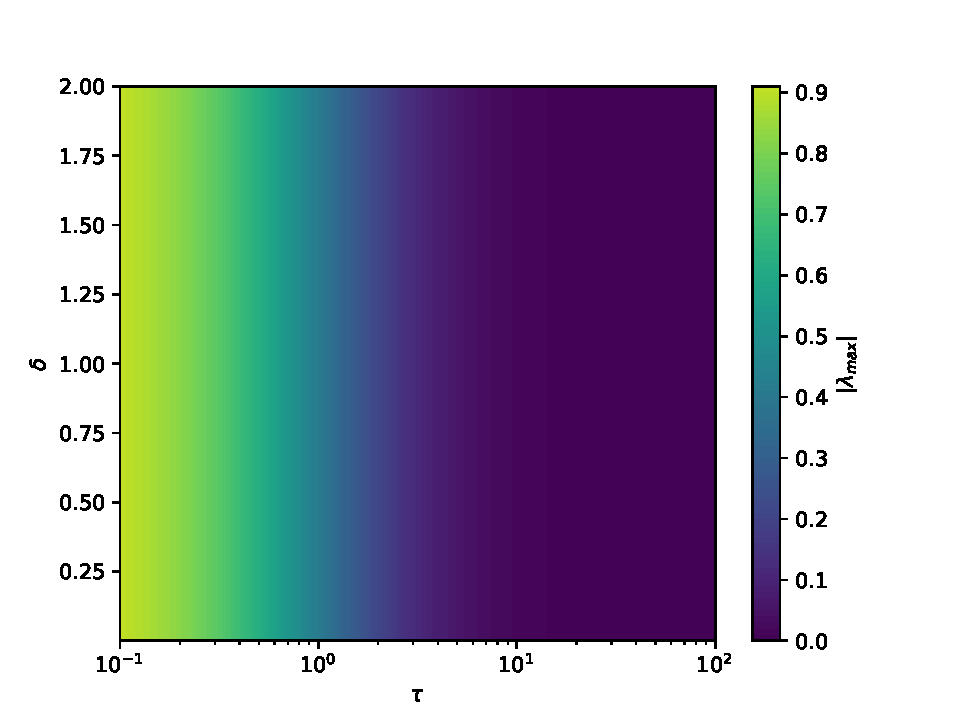
\includegraphics[width=0.9\linewidth]{deterministic/therefore_paper/therefore_figs/mb_scb.pdf}
    \caption{$|\lambda_{\max}|$ from numerically solved multiple balance time discretization and simple corner balance Fourier system over choices in mean free time ($\tau$) and cellular optical thickness ($\delta$) in S$_{16}$.}
    \label{fig:mb-scb}
\end{figure}

\subsection{Fourier analysis: OCI iterative scheme}
\label{sec:methods-faoci}
\newcommand{\exi}{e^{i\lambda\Sigma x_j}}
\newcommand{\omlp}{\omega^{(l+1)}}
\newcommand{\oml}{\omega^{(l)}}
\newcommand{\dx}{\Delta x}
\newcommand{\dt}{\Delta t}
\newcommand{\scatsum}{\sum^{M}_{n=0}}

To study the impact of time dependence on the convergence of an OCI iteration, we conduct a Fourier analysis on the error equation of an infinite-homogeneous medium model problem in slab geometry in a single time step.
Similar to the analysis in the previous section, we can assert that for an iteration scheme
\begin{equation}
    \Psi^{(l+1)} = \bm{T} \Psi^{(l)} \;,
\end{equation}
where $(l)$ is the iteration counter, convergence rate is
\begin{equation}
   \rho = \sup(|\bm{\lambda}_{\bm{T}}|)\;,
\end{equation}
 where $\lambda_{\bm{T}}$ contains the eigenvalues of $\bm{T}$ \cite{golub_matrix_1983, isaacson_numerical_1966}.
An iterative method will converge if and only if $\rho<1$. 
Furthermore, iterations converge faster for smaller $\rho$.

To derive the transport matrix $\bm{T}$ we can again use Fourier separation analysis on a model problem.
We first start by describing the absolute error of the angular flux at iteration step $(l)$
\begin{equation}
    \mathbf{f}^l = \Psi^{\text{converged}} - \Psi^l \;,
\end{equation}
and our Fourier ansatz on a functional form of that error
\begin{subequations}
    \label{eq:anz}
    \begin{align}
        f^{(l)}_{m,k,j,L/R} &= \omega^{(l)}a_{m,L/R}e^{i\lambda\Sigma x_j} \; ,
        &
        f^{(l)}_{m,k+1/2,j,L/R} &= \omega^{(l)}b_{m,L/R}e^{i\lambda\Sigma x_j} \;.
    \end{align}
\end{subequations} 
The upstream closures at the left boundary of the cell are
\begin{subequations}
\begin{equation}
    f_{m,k,j-1/2} =
    \begin{cases}
        f_{m,k,j-1, R} \;, & \mu > 0 \\
        f_{m,k,j, L} \;, & \mu < 0 
    \end{cases} \;,
\end{equation}
and at the right are
\begin{equation}
    f_{m,k,j+1/2} =
    \begin{cases}
        f_{m,k,j, R} \;, & \mu > 0 \\
        f_{m,k,j+1, L} \;, & \mu < 0 
    \end{cases} \;.
\end{equation}
\end{subequations}

Now, substitute the ansatz and upstream closures into the error form of Eq. \eqref{eq:scb-mb} and derive the eigensystem.
This is done by (1) collecting like terms, (2) dividing both sides by $\omega^{(l)} e^{i\Sigma x_j}$, (3) isolating terms with a remaining $\omega$ to the left-hand side, and finally (4) forming the eigensystem into the iteration matrix over all angular directions:
\begin{equation}
    \bm{T}_{OCI} = \left( 
    \bm{L}_c
    - \bm{S}
    \right)^{-1}
    \begin{bmatrix}
        \bm{L}_b^- & 0\\
        0 & \bm{L}_b^+
    \end{bmatrix} \;,
\end{equation}
which now forms a well-posed eigenvalue problem over all angles:
\begin{equation}
    \lambda\bm{a} = \bm{T} \bm{a} \; ,
\end{equation}
where the eigenvector $\mathbf{a}$ is defined by
\begin{equation}
    \mathbf{a} = \begin{bmatrix}
        a_{1} & a_{2} & \cdots & a_M
    \end{bmatrix} ^T \;,
\end{equation}
\begin{equation}
    a_m = \begin{bmatrix}
        a_{mR} & a_{mL} & b_{mR} & b_{mL} 
    \end{bmatrix} ^T \; ,
\end{equation}
$\bm{L}_c$ is the linear within-cell transport operator defined by Eqs.~\eqref{eq:Aja} and \eqref{eq:Aj}, 
\begin{equation}
    \bm{L}_b^+ = 
    \begin{bmatrix}
        0 & 0 & 0 & 0 \\
        -\mu_m e^{-i\lambda\sigma\dx} & 0 & 0 & 0 \\
        0 & 0 & 0 & 0 \\
        0 & 0 & -\mu_m e^{-i\lambda\sigma\dx} & 0
    \end{bmatrix} \; ,
\end{equation}
and
\begin{equation}
    \bm{L}_b^- = 
    \begin{bmatrix}
        0 & \mu_m e^{i\lambda\sigma\dx} & 0 & 0 \\
        0 & 0 & 0 & 0 \\
        0 & 0 & 0 & \mu_m e^{i\lambda\sigma\dx} \\
        0 & 0 & 0 & 0
    \end{bmatrix} \; .
\end{equation}
The scattering matrix is again akin to the previously described transport matrix in Eq.~\eqref{eq:scatter}.
Finally, to numerically evaluate the spectral radius we form the system for a given set of angles and weights from Gauss--Legendre quadrature and solve with \texttt{numpy.max(numpy.abs(numpy.linalg.eig(T)))} for $\omega \in [0,2\pi]$ at discrete points.
We vary the cellular optical thickness ($\delta =\Sigma \Delta x$), mean free time ($\tau = \Sigma v\Delta t$), and scattering ratio ($c=\Sigma_s/\Sigma$) to study convergence behavior in various physical regimes. 
The analogous eigensystem for source iteration is
\begin{equation}
    \bm{T}_{SI} = \left( 
    \bm{L}_c
    + \begin{bmatrix}
        \bm{L}_b^- & 0\\
        0 & \bm{L}_b^+
    \end{bmatrix}
    \right)^{-1}
    \bm{S} \; .
\end{equation} 
Section~\ref{sec:results-faoci} contains the results of this analysis.


\subsection{OCI multi-group transport}

We extend our single-energy derivations presented in Section~\ref{sec:methods-derv} to be energy dependent. 
Elements of the $\mathbf{S_{g' \rightarrow g}}$ matrix are now defined by
\begin{equation}
    \label{eq:scatter_mg}
   [\mathbf{S}_{g' \rightarrow g,j}]_{k.l} = \begin{cases}
			\frac{\Delta x_j \Sigma_{s,g'\rightarrow g,j}}{4}w_{\frac{|(r-s)|}{3}}, & \text{if $\mod{\frac{(r-s)}{3} =0}$}\\
            0, & \text{otherwise}
		 \end{cases} \; ,
%  \frac{\Delta x_j \Sigma_{s,j}}{4} w_n \; l=r k=s
\end{equation}
where $g' \rightarrow g$ indicates transfer from group $g'$ to group $g$ and $w$ are the quadrature weights. 
\begin{subequations}
The full system of linear equations in all groups and angles in cell $j$ becomes
\begin{equation}
    \bm{A}_j \bm{\Psi}_j = \bm{b}_j \; ,
\end{equation}
where
\begin{equation}
    \label{eq:fullOCIlhs}
    \bm{A}_j = 
    \begin{bmatrix}
        \bm{L}_{c,j,1} -\bm{S}_{1\rightarrow1,j} & -\bm{S}_{2\rightarrow1,j} & \cdots & \cdots& -\bm{S}_{G\rightarrow1,j}\\
        -\bm{S}_{1\rightarrow2,j} & \ddots & & & \vdots\\
         \vdots & & \bm{L}_{c,j,g}-\bm{S}_{g\rightarrow g,j} &  & \vdots\\
        \vdots & &  &  \ddots & \vdots \\
        -\bm{S}_{1\rightarrow G,j} & \cdots & \cdots & & \bm{L}_{c,j,G} -\bm{S}_{G\rightarrow G,j}
    \end{bmatrix} \; ,
\end{equation}
and Eqs.~\eqref{eq:rhs_sg} and \eqref{eq:x_vec} are extended to multi-group by
\begin{equation}
    \label{eq:fullOCIrhs}
    \bm{b}_j = 
    \begin{bmatrix}
        b_{j,1}, & b_{j,2}, & \cdots, & b_{j,G}
    \end{bmatrix} ^T 
\end{equation}
and
\begin{equation}
    \bm{\Psi}_j = 
    \begin{bmatrix}
        \Psi_{j,1}, & \cdots & \Psi_{j,g}, & \cdots, & \Psi_{j,G}
    \end{bmatrix} ^T \; ,
\end{equation}
 with otherwise similar structure.
\end{subequations}

\begin{figure}
    \centering
    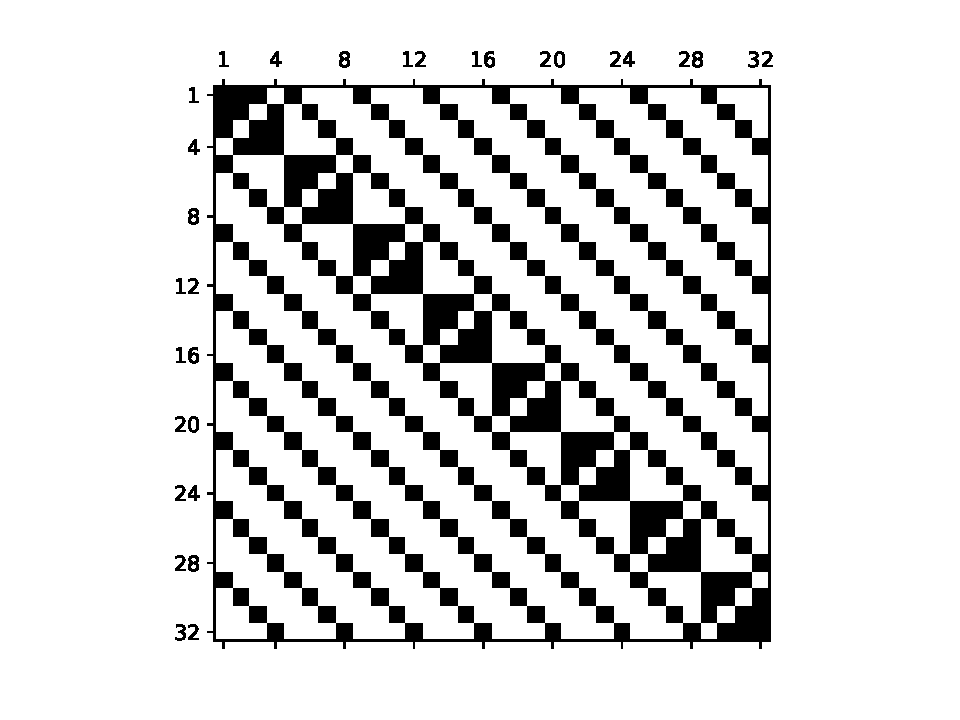
\includegraphics[width=.9\textwidth]{deterministic/therefore_paper/therefore_figs/spy.pdf}
    \caption{Sparsity pattern of a two group, four angle OCI $\bm{A}_j$ system generated for each cell.}
    \label{fig:spyA}
\end{figure}

Figure~\ref{fig:spyA} shows the structure of the within-cell system of equations arises from a two-group four-angle problem.
While $A_j$ does have significant sparsity, with an occupancy ratio of
\begin{equation}
    O_c = \frac{G(N+2)}{4NG} 
    \; ,
\end{equation}
which approaches 25\% with large angular and group counts, in this work we use dense representations in each cell because the matrix memory size for 1D transport is not limiting.

\subsection{Implementation on GPUs}

Implementing the OCI and SI approaches on GPUs requires a numerical linear algebra solver library like LAPACK~\cite{laug}.
Many high-performance open-source linear algebra tools exist (e.g., Trillinos \cite{trilinos-website}, PETSc \cite{petsc-user-ref}, MAGMA \cite{magma}), but we chose a vendor-supplied package depending on the hardware target of choice.
Our target hardware is an AMD MI250X so we use the AMD ROCm compute library to solve the system of equations.
Modern GPU vendor-supplied LAPACK libraries often include a \texttt{batched} class of solvers,
which operate on a group of like-sized systems in unison and are optimized by the hardware vendors.
For example, LU decomposition with pivoting (a generic direct solver for a system of linear equations) used in this work, comes from RocSolver's \texttt{strided\_batched\_dgesv} \cite{rocsolver}.

We use direct solvers here because all systems are relatively small, with orders ranging between 4 and 100.
This makes the use of a batched implementation of LU decomposition with pivoting ideal.
Furthermore, LAPACK-type implementations of \texttt{\_gesv} (\textbf{GE}neral linear \textbf{S}ol\textbf{V}e)  automatically return the $L+U+D$ decomposition of a generic matrix $A$.
So, in subsequent iterations, this system can be back solved quickly (using LAPACK \texttt{\_getrs}).
In this mode for both SI and OCI, the only user-defined device kernels are the RHS vector builders which are already memory safe operations.

This software engineering design will increase the memory footprint of OCI and SI as the $LHS$ matrices are stored in memory.
This is acceptable for 1D transport but more optimization may be required when moving to 2D and 3D solvers.

Algorithm \ref{alg:si} describes the convergence loop for source iteration.
$\mathbf{L}_{c,j,g,m}$ and $\bm{d}_{j,g,m}$ matrices are always of dimension $4\times 4$ and 4, respectively, for our space time-discretization scheme and are defined in Appendix~\ref{app:source_iteration}.
The number of systems to solve changes with the number of angles ($N$), groups ($G$), and cells ($J$).
In this algorithm the number of systems solved in parallel at one spatial index $j$ is $N \times G$.
SI requires host-side dispatching in every cell to execute the sequential nature of the sweep.
We implemented this algorithm to do all available computing at once (negative sweeps are happening in unison with positive ones in all angles and groups).
The angle parallelism exploited for this implementation of SI on the GPU is enabled by the \texttt{strided\_batched} call itself.
Thus, the traditional loop over all angles is implemented by the solver, not explicitly by the user.
Group-to-group communication is done at the end of every iteration.
The first iteration calls the full \texttt{\_gesv} algorithm, which returns the solution of the system and the $L+U+D$ decomposition in $A$.
Subsequent iterations just perform a back substitution (\texttt{\_getrs}).
Profiling shows that host functions (including host$\rightarrow$device and device$\rightarrow$host communication) account for up to around $9\%$ of the runtime in the largest problems we considered.

\SetKwComment{Comment}{//}{ }
\DontPrintSemicolon
\begin{algorithm}
    build $\mathbf{L}_{c,j,g,m}$ for each cell, angle, and group \Comment*[r]{Eq. \ref{eq:app:si_sys}}
    
    move $\mathbf{L}_{c,j,g,m}$ to device

    $\beta$ = $4NG$ \Comment*[r]{offset to a cell} %\Comment*[r]{offset to a cell}

    $l = 0$ \Comment*[r]{iteration counter}

    converged = false

    \While{!converged}{

    build constant part of $\bm{d}_{j,g,m}$ in all cells, angles, and groups \Comment*[r]{Eq. \eqref{eq:app:si_rhs}}

    move constant part of $\bm{d}_{j,g,m}$ to device
        
        \For{j = 0 to $J$ \Comment*[r]{parallel over groups and angles}}{ 

            build variable part of $\bm{d}_{j,g,m}$ at cells $j$ and $J-j$  \Comment*[r]{on GPU Eq. \eqref{eq:app:si_rhs}}

            \If{l=0}{
                \Comment*[r]{LHS in, L+U+D out}
                $\Psi_j$ = \texttt{GPU\_strided\_batched\_dgesv}($\mathbf{L}_{c,j}$[$\beta^{2}j$],$\bm{d}_{j}$[$\beta j$])
            }\Else{
                \Comment*[r]{back substitution}
                $\Psi_j$ = \texttt{GPU\_strided\_batched\_dgetrs}($\mathbf{L}_{c,j}$[$\beta^2j$],$\bm{d}_{j}$[$\beta j$]) 
            }
            }

        move $\Psi$ to Host

        $\bm{\phi}^l =\sum_{n=1}^{N} w _n\Psi^{l}_{n}$ \Comment*[r]{Eq. \eqref{eq:app:si_sf}}

        $e=||\bm{\phi}^l - \bm{\phi}^{l-1}||_2$

        $\rho_e = e^l / e^{l-1}$

        \If{$e < \epsilon(1-\rho_e)$}{
            converged = true
        }

        $e^{l-1} = e^l$ 

        $l++$
        
        move $\Phi^l$ to Host

        communicate group to group \Comment*[r]{Eq. \eqref{eq:app:si_update}}

    }
    \vspace{1.5em}
    \caption{Source iteration algorithm implemented on GPU where $\bm\phi$ is scalar flux. Equations in Appendix~\ref{app:source_iteration}. Simplified for brevity.}
    \label{alg:si}
\end{algorithm}

Algorithm \ref{alg:ocigpu} describes OCI's on-GPU convergence loop.
We found OCI to be more sensitive to within-iteration optimizations.
In some cases (specifically in the thin limit) OCI may require significantly more iterations to converge.
For that reason, it is imperative that the OCI iteration take place entirely on the GPU.
Luckily, OCI's algorithm is simpler to implement on GPUs because group-to-group communication happens within the solved systems.
We implemented the following algorithm to do that: everything under the \texttt{while} loop is wholly contained on the GPU, requiring minimal device-to-host communication.

\begin{algorithm}
    
    build $\bm{A}_j$ in all cells and move to device \Comment*[r]{Eq.~\eqref{eq:fullOCIlhs}}

    build constant part of $\bm{b}_j$ in all cells and move to device \Comment*[r]{Eq.~\eqref{eq:fullOCIrhs}}

    $l = 0$ \Comment*[r]{iteration counter}

    converged = false

    \While{!converged}{
        \Comment*[r]{incident angular fluxes from previous iteration}
        \Comment*[r]{user-defined GPU kernel}
        build variable part of $\bm{b}_j$ in all cells \Comment*[r]{Eq.~\eqref{eq:fullOCIrhs}}

        \If{l=0}{
            \Comment*[r]{A in-out becomes the L+U+D decomp}
            $\Psi$ = \texttt{GPU\_strided\_batched\_dgesv}($A$,$b$)
        }\Else{
            \Comment*[r]{back substitution}
            $\Psi$ = \texttt{GPU\_strided\_batched\_dgetrs}($A$,$b$) 
        }

        $e=||\Psi^l - \Psi^{l-1}||_2$ \Comment*[r]{Done on GPU using rocBLAS dr2n}

        $\rho_e = e^l / e^{l-1}$ \Comment*[r]{spectral radius estimation}

        \If{$e < \epsilon(1-\rho_e)$\Comment*[r]{controlling for false convergence}} { 
            converged = true
        }

        $e^{l-1} = e^l$

        $b^{l-1} = b^l$

        $l++$
            
    }
    
    move $\Psi$ to host

    \vspace{1.5em}
    
    \caption{One-cell inversion algorithm implemented on GPUs. Simplified for brevity.}
    \label{alg:ocigpu}
\end{algorithm}

OCI's systems are represented as dense within a cell and built in a strided-batched configuration to take advantage of the block sparsity.
However, now systems within an iteration can be dispatched in unison.
Just as with the SI algorithm, the GPU strided batched solver implements the parallel loop over all cells.
The intra-iteration $b$-vector production kernels are the only user-defined device functions required in this algorithm. These are relatively simple to implement as they are thread-safe operations.


\section{Results}
\label{sec:results}

In this section, we show results that support our initial conjecture that OCI convergence accelerates, more than SI, in transient transport calculations with decreased time step sizes.
We also further analyze OCI's performance on AMD MI250X GPUs using batched LAPACK solvers on a highly scattering problem from literature at multiple time step sizes and cell width values.

\subsection{Fourier analysis: transient iterative convergence rate}
\label{sec:results-faoci}

To study the impact of transient conditions on OCI we solve the Fourier system for steady-state and time-dependent transport derived in Section~\ref{sec:methods-faoci} both for simple corner balance in space.
For all Fourier analyses we sample $\lambda \in [0,2\pi]$ at \num{250} points and use \texttt{numpy.max(numpy.abs(numpy.eig(}$T$\texttt{)))} to compute spectral radius at a given point in parameter space ($\delta$ ($\Sigma\Delta x$), $\tau$ ($\Sigma v\Delta t$), and $c$ ($\Sigma_s$/$\Sigma$)) in S$_{8}$ using Gauss--Legendre quadrature.

Table~\ref{table:difflimit} shows spectral radii produced from steady-state and transient OCI systems with various choices of mean free time ($\tau$), at various cellular optical thicknesses ($\delta$).
Steady-state predictions show the expected and previously published results that $\rho=1$ when $c=1$ regardless of $\delta$.
However, for the time-dependent system, $\rho<1$ regardless of the considered $\tau$ and $\delta$.
Furthermore, as $\tau$ shrinks and $\delta$ grows, $\rho$ dramatically decreases, approaching zero at the smallest $\tau$ and largest $\delta$.

\begin{table}
  \centering
  \begin{tabular}{@{}l c c c @{}} \toprule
    $\tau$ & $\delta=10.$ & $\delta=1.0$ & $\delta=0.1$ \\ \midrule
    SS  & \num{1.0000} & \num{1.0000} & \num{1.0000} \\
    10 & \num{0.99522} & \num{0.99952} & \num{0.99995} \\
    1  & \num{0.95323} & \num{0.99522} & \num{0.99952} \\
    0.1   & \num{0.64031} & \num{0.95321} & \num{0.99522} \\
    0.01 & \num{0.11177} & \num{0.63343} & \num{0.95351} \\
    \bottomrule
  \end{tabular}
  \caption{OCI spectral radius $\rho$ in the diffusive limit ($c=\Sigma_s/\Sigma =1.0$) from Fourier analysis at various mean free time ($\tau$) and cellular optical thickness ($\delta$) values. SS indicates steady state.} 
  \label{table:difflimit} 
\end{table}

Figure~\ref{fig:specrad_fa} shows $\rho$ predictions for OCI and SI produced from the Fourier system.
As previously published: as $\delta$ gets smaller, $\rho$ approaches 1 regardless of the scattering ratio.
As postulated in this work: as $\Delta t$ gets smaller, $\rho$ tends to 0---due to improvements in scattering ratio (which also affects SI) and increasing $\delta$---increasing the diagonal dominance of the iteration matrix.

\begin{figure}
    \centering
    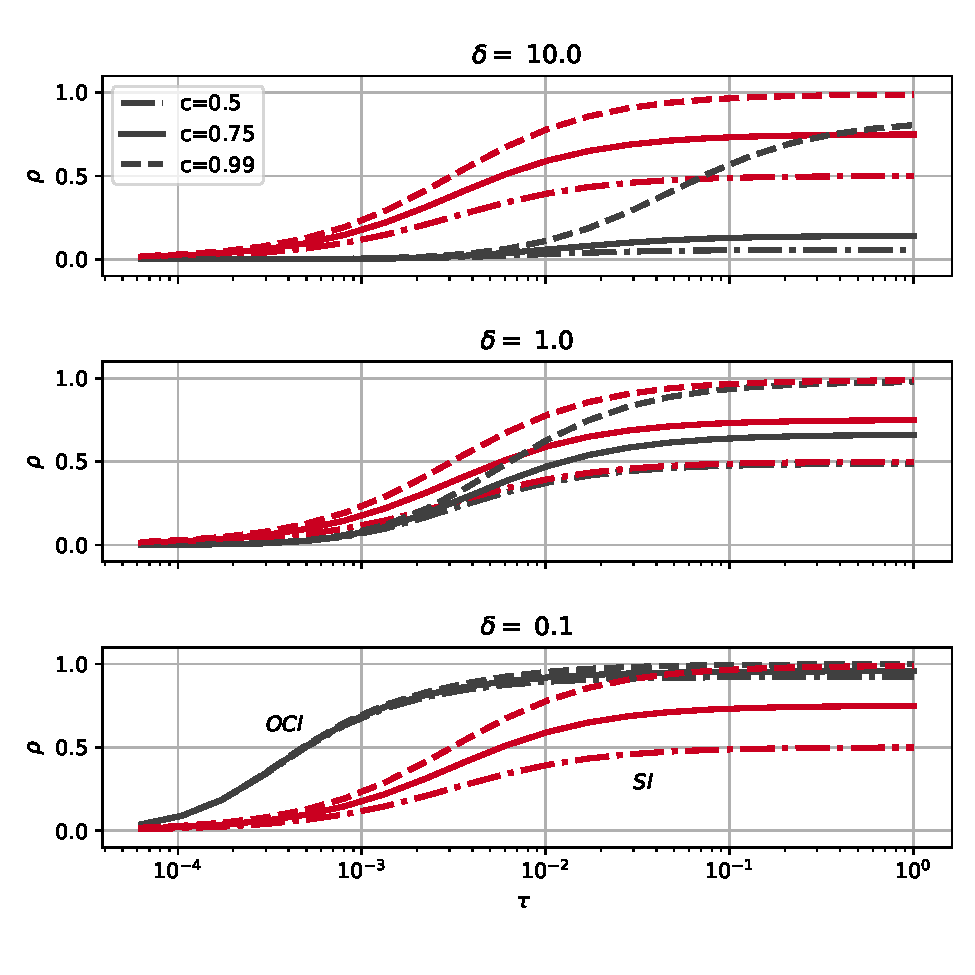
\includegraphics[width=\textwidth]{deterministic/therefore_paper/therefore_figs/spec_rad_over_dt.pdf}
    \caption{Spectral radius of OCI (black) and SI (red) over choices of mean free path ($\delta$), time step ($\Delta t$), and scattering ratio ($c$).}
    \label{fig:specrad_fa}
\end{figure}

Fourier analysis results also show that, depending on the location in parameter space, the dominant eigenvalue ($|\lambda_{max}|$) can have large imaginary components, with positive or negative real components and complex conjugate reflections over the real axis.
Complex dominant eigenvalues leading to oscillatory convergence patterns have previously been identified in spatial domain decomposition algorithms where $\rho=1$ when $\delta \rightarrow 0$ \cite{compeig2019ani}. 

Deterministic solvers are commonly verified against predictions of $\rho$ from Fourier analysis.
We attempted to do the same by running a problem with length \SI{100}{\centi\meter}, vacuum boundary conditions, a convergence tolerance of \num{1e-13}, $\Sigma=$ \SI{2.5}{\per\centi\meter}, $\Delta x=$ \SI{0.10}{\centi\meter}, $c=$ \num{0.9}, $\Delta t=$\SI{0.10}{\s}, $v=$ \SI{4.0}{\meter\per\s} ($\delta =$ \num{0.25}, $\tau=$ \num{1.0}), a random (uniform [0,1]) initial guess for the angular flux, and no material source in S$_8$.
The random initial guess excites all error modes and provides an anaclitic solution ($\Psi^{\text{converged}} = \bm{0}$) to compute iteration errors.
Figure \ref{fig:eigplot} on the left shows the predicted eigenvalues from Fourier analysis and indicates the dominant eigenvalue that contributes to $\rho$ for this particular problem.
In this case, that dominant eigenvalue has considerable real and complex components at $\lambda_{max} =$ \num{0.429} $+$ \num{0.216}$i$ and $\rho=$ \num{0.4831}.

Figure~\ref{fig:eigplot} on the right shows $\rho$ predicted from Fourier analysis (flat constant line) as well as $\rho$ measured from the ratio of subsequent residuals as a function of iteration count ($l$).
The empirically estimated value of $\rho$ oscillates around the predicted spectral radius until convergence, with a measured amplitude around \num{0.1}.
The oscillation of the empirically measured spectral radius also seems to grow through iteration count, which may be due to the compounding impact of truncation error and/or machine precision.
So, we cannot rigorously verify our implementation of OCI via Fourier results, because only a mean of the oscillation will match the only-real $\rho$ provided from Fourier results ($|\lambda_{max}|$).
More work is warranted to develop methods that can better capture the empirical behavior of the ratio of subsequent residuals produced from a transport solver and relate them to the complex dominant eigenvalues that may be predicted from Fourier analysis.

\begin{figure}
    \centering
    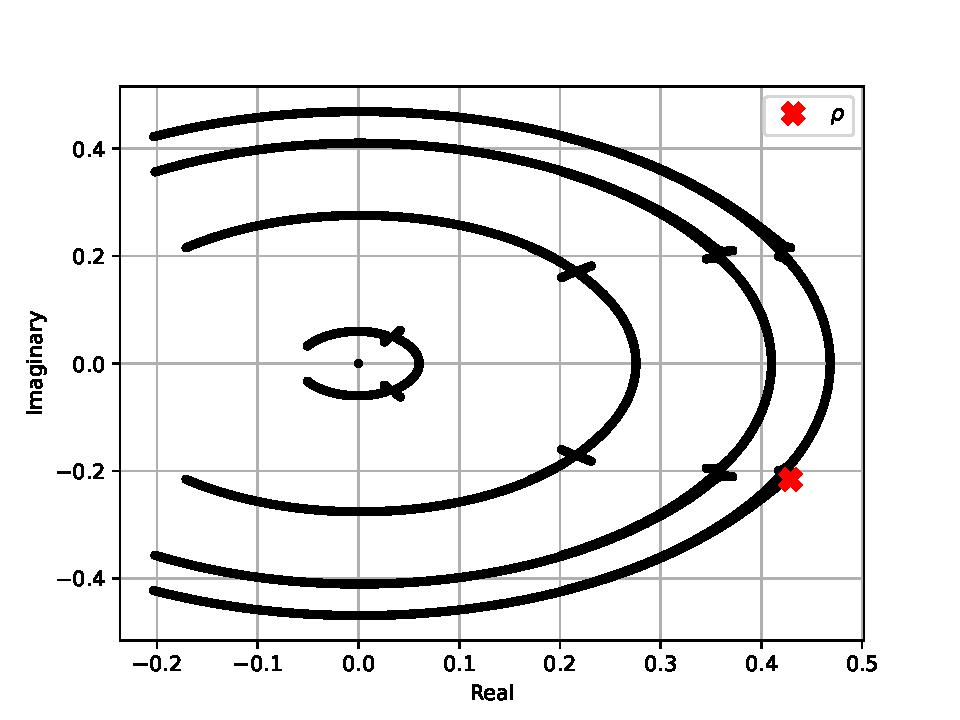
\includegraphics[width=.49\textwidth]{deterministic/therefore_paper/therefore_figs/eig_plot.pdf}
    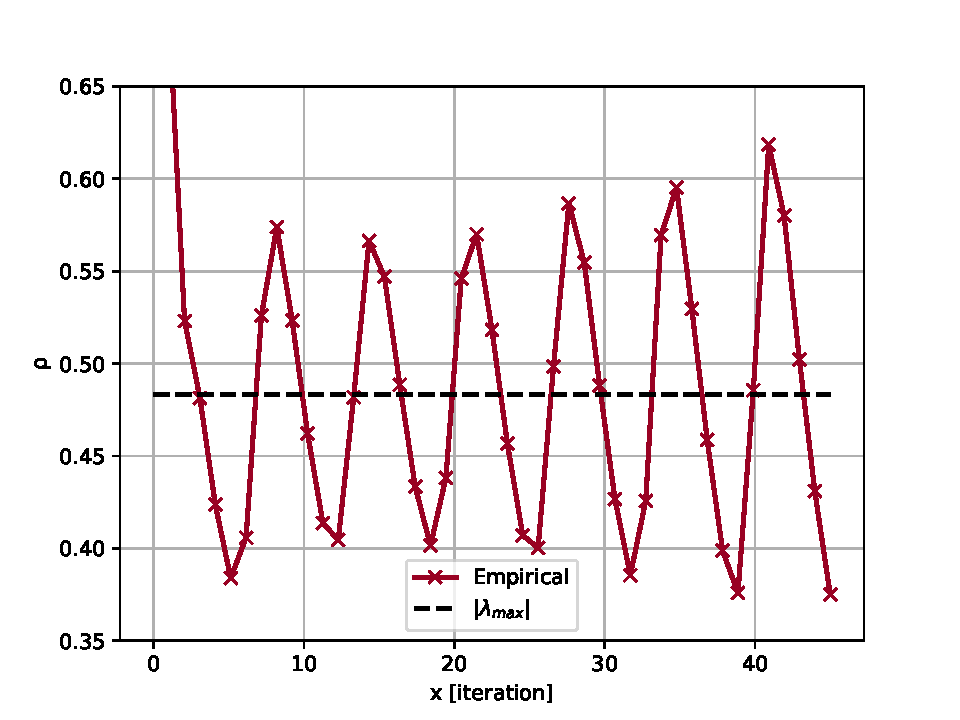
\includegraphics[width=.49\textwidth]{deterministic/therefore_paper/therefore_figs/eig_spec_rad.pdf}
    \caption{Eigenvalues in the complex plane of OCI (left), and spectral radius as a function of iteration from the empirical ratio of subsequent residuals and as predicted by Fourier analysis (right).}
    \label{fig:eigplot}
\end{figure}

\subsection{Performance on GPUs}

Runtime results were gathered on the Tioga machine at Lawrence Livermore National Laboratory.
Tioga is an early access machine for LLNL's exascale-class El Capitan machine.
On its standard partition, Tioga's nodes have four AMD MI250X GPUs and one AMD EPYC 7A53 CPU.
Our methods are currently implemented for a single GPU, so this analysis will be limited to using a single graphics compute die of an MI250X.
We compiled using ROCm version 6.2.1 (includes rocSOLVER and rocBLAS libraries) and used double precision for all values represented.

To analyze performance, we adapt a test problem described by \cite{rosa_cellwise_2013} for a 1D time-dependent, multi-group problem.
Table~\ref{table:rosa_test} describes the material data for this 
two-group problem ($L=$ \SI{100}{\centi\meter}) with vacuum boundary conditions on either side. 
The initial condition is $\psi_{t=0} = 0$, and we analyze runtime performance over various choices of $\delta$ and quadrature order at time step sizes of $\Delta t=$ \SI{0.1}{\s} and \SI{10.0}{\s}.
The problem is highly scattering with a maximum scattering ratio of \num{0.99997}.


\begin{table}
  \centering
  \begin{tabular}{@{}c c c c c c@{}} \toprule
    Property & Group 1 & Group 2 & units \\ \midrule
    $\Sigma$ & 1.5454 &  0.45468 & cm$^{-1}$  \\
    $\Sigma_{s,g\rightarrow g}$  & 0.61789 &  0.0072534 & cm$^{-1}$  \\
    $\Sigma_{s,g'\rightarrow g}$  & 0.38211 &  0.92747 & cm$^{-1}$ \\
    $\Sigma_s/\Sigma$ & 0.99997 & 0.86012 & - \\
    $Q$ & 1 & 1 & cm$^{-3}$s$^{-1}$\\
    $v$ & 1 & 0.5 & cm s$^{-1}$ \\
    \bottomrule
  \end{tabular}
  \caption{Test problem material data and simulation parameters.}
  \label{table:rosa_test} 
\end{table}

Figure~\ref{fig:runtimes10.0} on the left compares the wall clock runtime of OCI (in black) and SI (in red) over various selections of $\delta$ (controlled via $\Delta x$) with $\Delta t=$ \SI{10.0}{\s}, Figure~\ref{fig:runtimes10.0} on the right shows the speedup of OCI over SI.
In each row, we are increasing quadrature order to increase the overall dimensionality of the system.
Figure \ref{fig:runtimes0.1} shows the same information, but for $\Delta t=$ \SI{0.1}{\s}.
Runtimes are measured over the convergence loops (see Algorithms \ref{alg:si} and \ref{alg:ocigpu}), so do not include the building and moving the $A_j$ matrices from host to device.
The total cross section used in the $\delta$ scale is the limiting value (the smallest) from group 2 (see Table \ref{table:rosa_test}).

SI's convergence loop runtime increases linearly as cellular optical thickness decreases as there are more cells to solve  in serial.
The number of iterations required to converge the solution is the same but the size of the solution grows.
SI only has $NG$ $4\times4$ systems to solve at any moment so the amount of serial work increases with the number of cells (decreasing $\delta$).
However, as we increase quadrature order the runtime performance of SI actually improves because the solver has more parallelizable degrees of freedom.

\begin{figure}
    \centering
    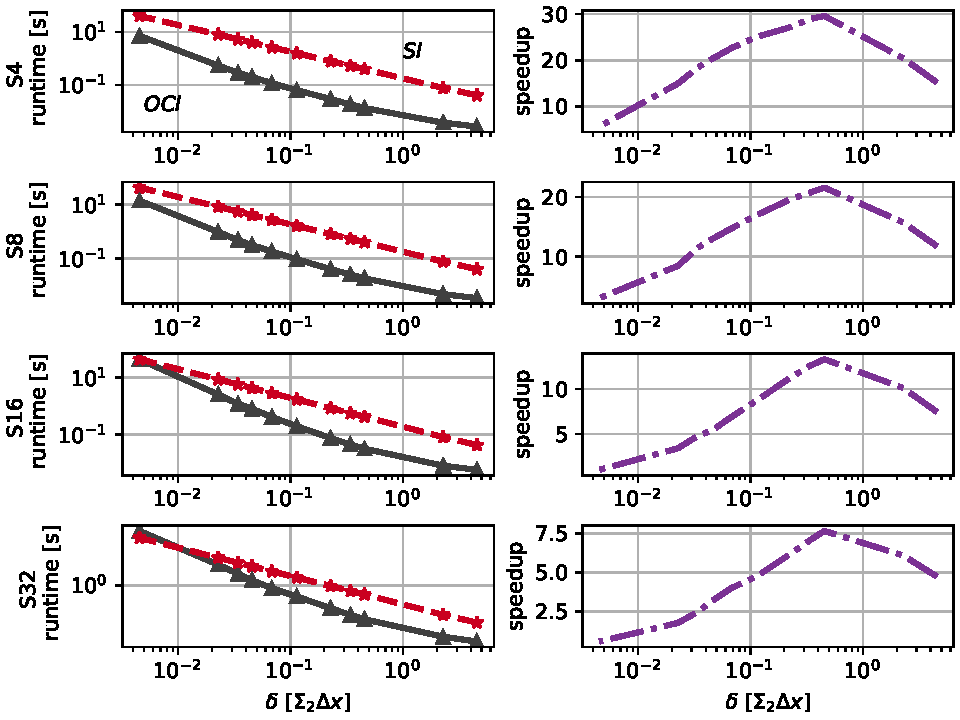
\includegraphics[width=1.0\textwidth]{deterministic/therefore_paper/therefore_figs/runtimes_10.0.pdf}
    \caption{Wall-clock runtimes of the convergence loop (left) and 
    speedup of OCI over SI (right) at $\Delta t=$\SI{10.0}{\s} ($\tau=$ \num{2.2734}) as a function of $\delta$ and at various quadrature orders.}
    \label{fig:runtimes10.0}
\end{figure}

\begin{figure}
    \centering
    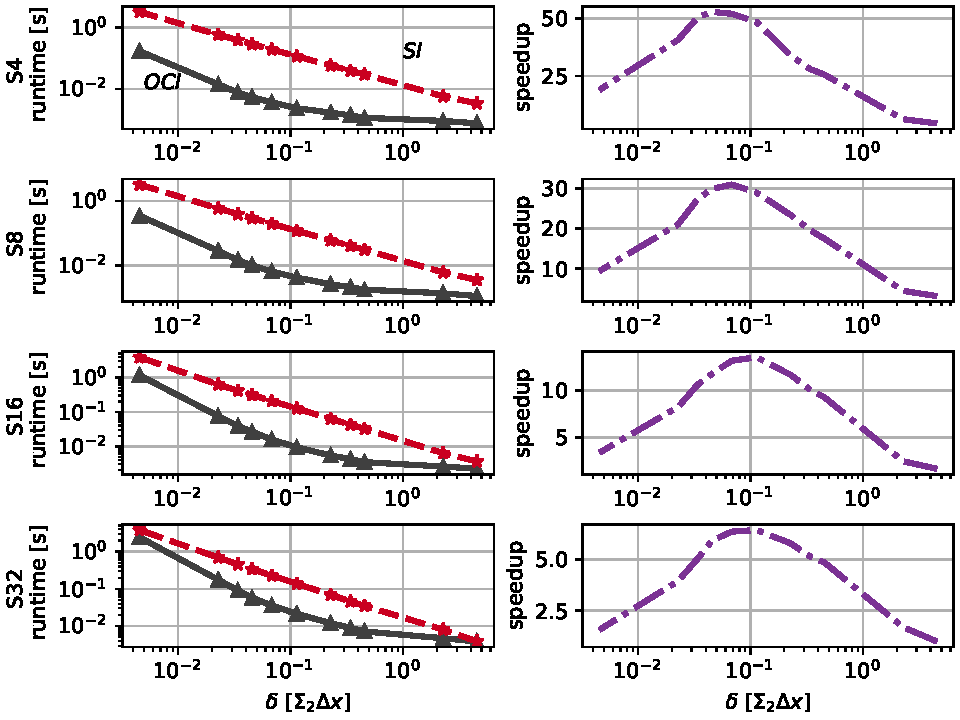
\includegraphics[width=1.0\textwidth]{deterministic/therefore_paper/therefore_figs/runtimes_0.1.pdf}
    \caption{Wall-clock runtimes of the convergence loop (left) and 
    speedup of OCI over SI (right) at $\Delta t=$\SI{0.1}{\s} ($\tau=$ \num{0.0227}) as a function of $\delta$ and at various quadrature orders.}
    \label{fig:runtimes0.1}
\end{figure}

For larger time steps, OCI shows less speed-up over SI as it slows for S$_{16}$ and S$_{32}$ quadratures in the thin limit.
The parallelizable degrees of freedom increase with the number of cells (by decreasing $\delta$), but the spectral radius decreases dramatically as cells get thinner.
In the thin limit, OCI requires more iterations to converge the solution, but those iterations can be done faster on the GPU than with SI.
OCI seems to have a ``sweet spot'', where the size of the matrices is optimal for the solver, before the spectral radius degrades in the thin limit.
This is observed at around $\delta=4$ for $\Delta t=$ \SI{10}{\s} and $\delta=0.1$ for $\Delta t=$ \SI{0.1}{\s}.
The location of this optimality depends on factors including optimizations at the solver level employed when compiling the vendor-supplied LAPACK libraries \cite{rocsolver}.
The smaller time step increases OCI's relative performance over SI, generally increasing speedup by upwards of 40\% for this highly scattering problem.

\section{Discussion}

% transient patterns 
The 1D convergence trends we present here agree with
previously published 2D steady-state Fourier results for OCI schemes 
(i.e., $\rho\rightarrow1$ as $\delta\rightarrow0$) \cite{rosa_cellwise_2013, man1994parallel}.
This leads us to expect that the relationship between mean free time and spectral radius will persist in higher spatial dimensions, 
but exactly how much dynamic impacts to OCI decrease $\rho$ in 2D transport has yet to be shown.

% preconditioned FPS v OCI in 3D
Parallel sweeping algorithms may not be well suited to GPUs where non-uniform work distributions come with significant overhead. 
Available results for full parallel sweeps on GPUs show that even optimized applications underperform relative to the theoretical hardware resources available \cite{Thomas_2024_profiling, wolfe2022roofline, kunen_kripke_2015, womeldorff_taking_2017, zerr_partisn_2019}.
On the other hand, space-parallel OCI uses the same parallel scheme in 2D and 3D as it does in 1D, with arithmetically intense operations that align well with the GPU parallelism paradigm.
So, we hypothesize that OCI can better take advantage of the compute resources available on GPUs in higher dimensions than full-parallel-sweep SI on GPUs, but this requires further study.

Production SI codes that simulate high-fidelity 3D models never form the actual iteration matrix, resulting in significant memory efficiency~\cite{partisn, evans_denovo_2010, kunen_porting_2019, MINARET, wang_necp_hydra_2020, ShemonEmilyR.2016PUM}.
Our implementation of OCI is not memory efficient, because we store the strided batched representation of the entire linear system for the iteration algorithm.
While this block-sparse representation does dramatically save memory, more optimizations to OCI may be needed when moving to 3D.
For example, OCI forms the iteration matrix as a linear operator.
Many algorithms exist to solve systems of linear operators without ever forming the matrix.
Libraries already exist to do this on CPUs and GPUs (e.g., LibCEED \cite{libceed-joss-paper}).
Even more simple optimization may involve using sparse representations for the cell blocks themselves and sparse direct solvers.


OCI algorithms may be better suited for domain-decomposed simulations (required for distributed-memory parallelism) than SI.
Some KBA algorithms can degrade with large processor counts \cite{baker_kba_2017}.
For a hypothetical OCI algorithm, communication between subdomains can be very organized, occurring at every iteration (or after a specified number of iterations) at the same time as all other subdomains.
This may lead to superior weak scaling across large decomposed problems on distributed (MPI) type systems.
Many parallel domain decomposition algorithms are already based on the same underlying parallel block Jacobi, Gauss--Seidel, or red-black iterations as OCI \cite{anistratov_iterative_2015, compeig2019ani}.

While this work is limited to AMD GPUs and the ROCm software stack, our implementation of OCI is portable to other GPU types.
In fact, the workflow present in OCI---solving many small dense or sparse linear algebra systems in parallel---is common in much numerical software.
We expect that these types of solvers will exist when porting to a new hardware accelerator used for scientific computing.
For example, Nvidia's cuSOLVER \cite{cuSovler} and Intel's oneMKL \cite{oneMKL} both implement strided batched versions of LU decomposition with pivoting for their GPUs.
Porting the OCI algorithm presented in Algorithm~\ref{alg:ocigpu} to another GPU would just require altering names of solver function calls, compiler commands, and switching out library header imports.

OCI algorithms may also be well suited for modeling anisotropic scattering distributions because all angles are computed at once in every cell.
On unstructured meshes, OCI algorithms avoid one challenge for sweep-based methods: when groups of cells have cyclic dependencies (i.e., when an incident transport angle is parallel to a cell boundary).

% OCI's need for a perfomant preconditioner
Regardless of how well an implementation of any OCI scheme performs, the inability to converge problems in the thin limit regardless of scattering ratio will continue to lead to lackluster performance in some problems.
In this work, we compared unpreconditioned SI to unpreconditioned OCI using fixed-point iterations.
When in production, SI typically uses a well-accepted set of acceleration schemes/preconditioners (most popularly diffusion synthetic acceleration) accompanied by Krylov subspace methods.
Likewise, some acceleration/preconditioning or Krylov methods may exist that can help OCI more-rapidly converge in the thin limit, while not significantly degrading the space-parallel performance of OCI.

Acceleration schemes for OCI have previously been explored, including transport synthetic acceleration \cite{tsa2009rosa} and using hybrid schemes with OCI and traditional SI \cite{hoagland_hybrid_2021}.
Both resynchronize cells by sweeping to improve convergence; however, the resulting algorithms are no longer space-parallel and involve a potentially more-expensive sweep operation.

\section{Conclusions and Future Work}

We derived the multiple balance and simple corner balance time-space discretization schemes and demonstrated, with Fourier analysis, that our time iteration method is unconditionally stable.
We also derived eigensystems for one-cell inversion and source iteration, showing that one-cell inversion iterations converge faster as mean free time shrinks.
Furthermore, OCI's convergence rate improves faster than SI's with decreasing mean free time.
We confirmed this with both Fourier and empirical analysis of implemented one-cell inversion and source iteration solvers.
Although we only explored block Jacobi OCI, we also expect this behavior to improve convergence of time-dependent block Gauss--Seidel OCI.

When more iterations are required to converge problems of interest---particularly in highly scattering and optically thin problems---OCI can run individual iterations significantly faster than SI when using batched direct solvers on GPUs from vendor-supplied libraries.
For OCI the number of on-device performant compute kernels is limited to data-parallel matrix-building operations, with all other compute kernels being called from optimized libraries. 
While optimization could improve both the OCI and SI algorithms, we analyzed performance to ensure there was little computational overhead from data movement and user-defined kernels.

Moving forward, we are exploring synthetic acceleration techniques to preserve the OCI space-parallel performance on GPUs while ameliorating issues in the thin and scattering limits.
Space-parallel OCI schemes offer promise as a high-performing class of iterative solvers for time-dependent radiation transport on modern heterogeneous compute architectures.

\section*{Acknowledgments}

The authors thank Dmitriy Anistratov of North Carolina State University for useful conversations about Fourier analysis results, James Warsa of Los Alamos National Laboratory for useful conversations about previous work and Damon McDougall of Advanced Micro Devices for support using ROCm compilers and profilers. 
The authors also thank the high performance computing staff at Lawrence Livermore National Laboratory for support using the Tioga machine.

This work was supported by the Center for Exascale Monte Carlo Neutron Transport (CEMeNT), a PSAAP-III project funded by the Department of Energy, grant number: DE-NA003967.

\section*{Appendix: Source Iteration Systems}
\label{app:source_iteration}

\newcommand{\lph}{^{(l+1/2)}}
\newcommand{\lp}{^{(l+1)}}


Using a source iteration to solve a multi-group problem with multiple balance in time \cite{variansyah_robust_2021} and simple corner balance in space \cite{adams_subcell_1997} gives a $4\times 4$ system of linear equations:
\begin{equation}
    \label{eq:app:si_sys}
    \mathbf{L}_{c,j,g,m} \begin{bmatrix}
    \psi_{m,k,g,j,L}\lph \\
    \psi_{m,k,g,j,R}\lph \\
    \psi_{m,k+1/2,g,j,L}\lph \\
    \psi_{m,k+1/2,g,j,R}\lph
    \end{bmatrix}
    = \mathbf{d}_{j,m,g} \;,
\end{equation}
solved in every angle and group by sweeping from cell to cell,
where $\mathbf{L}_{c,j,g,m}$ is from Eq. \eqref{eq:Aj}
and
\begin{subequations}
\label{eq:app:si_rhs}
\begin{equation}
    \mathbf{d}_{j,g,m} = 
    \begin{cases}
        \bm{d}_{j,g,m}^+ & \mu_m>0 \\
        \bm{d}_{j,g,m}^- & \mu_m<0 \\
    \end{cases} \;,
\end{equation}
where
\begin{equation}
   \bm{d}_{j,g,m}^+ = \begin{bmatrix}
    \frac{\Delta x_j}{4} \left( \Sigma_{s,g\rightarrow g,j} \phi_{k,g,j,L}^{(l)}  +   Q_{k,j,L} \right) + \frac{\Delta x_j}{2 v_g \Delta t} \psi_{m,k-1/2,g,j,L} + \mu_m \psi_{m,k,g,j-1,R}\lph \\
    \frac{\Delta x_j}{4} \left( \Sigma_{s,g\rightarrow g,j} \phi_{k,g,j,R}^{(l)}  +   Q_{k,j,R} \right) + \frac{\Delta x_j}{2 v_g \Delta t} \psi_{m,k-1/2,g,j,R} \\
    \frac{\Delta x_j}{4} \left( \Sigma_{s,g\rightarrow g,j} \phi_{k+1/2,g,j,L}^{(l)}  +   Q_{k+1/2,j,L} \right) + \mu_m \psi_{m,k+1/2,g,j-1,R}\lph \\
    \frac{\Delta x_j}{4} \left( \Sigma_{s,g\rightarrow g,j} \phi_{k+1/2,g,j,R}^{(l)}  +   Q_{k+1/2,j,R} \right) 
    \end{bmatrix} \;,
\end{equation}
\begin{equation}
   \bm{d}_{j,g,m}^- = \begin{bmatrix}
    \frac{\Delta x_j}{4} \left( \Sigma_{s,g\rightarrow g,j} \phi_{k,g,j,L}^{(l)}  +   Q_{k,j,L} \right) + \frac{\Delta x_j}{2 v_g \Delta t} \psi_{m,k-1/2,g,j,L}  \\
    \frac{\Delta x_j}{4} \left( \Sigma_{s,g\rightarrow g,j} \phi_{k,g,j,R}^{(l)}  +   Q_{k,j,R} \right) + \frac{\Delta x_j}{2 v_g \Delta t} \psi_{m,k-1/2,g,j,R} - \mu_m \psi_{m,k,g,j+1,L}\lph  \\
    \frac{\Delta x_j}{4} \left( \Sigma_{s,g\rightarrow g,j} \phi_{k+1/2,g,j,L}^{(l)}  +   Q_{k+1/2,j,L} \right)  \\
    \frac{\Delta x_j}{4} \left( \Sigma_{s,g\rightarrow g,j} \phi_{k+1/2,g,j,R}^{(l)}  +   Q_{k+1/2,j,R} \right) - \mu_m \psi_{m,k+1/2,g,j+1,L}\lph
    \end{bmatrix} \;,
\end{equation}
and $\phi$ is the scalar flux.
\end{subequations}
After sweeping the mesh cells in the appropriate directions for each angle in the quadrature set and every group, the scalar flux vector can be updated via
\begin{equation}
\label{eq:app:si_sf}
\bm{\phi}_{k,g,j}\lph = 
\begin{bmatrix}
    \phi_{k,g,j,L}\lph \\
    \phi_{k,g,j,R}\lph \\
    \phi_{k+1/2,g,j,L}\lph \\
    \phi_{k+1/2,g,j,R}\lph
    \end{bmatrix}   = \sum\limits_{n=1}^N w_n 
    \begin{bmatrix}
    \psi_{n,k,g,j,L}\lph \\
    \psi_{n,k,g,j,R}\lph \\
    \psi_{n,k+1/2,g,j,L}\lph \\
    \psi_{n,k+1/2,g,j,R}\lph
    \end{bmatrix} \;.
\end{equation}
Then, group-to-group communication can be computed with
\begin{equation}
    \label{eq:app:si_update}
    \bm{\phi}_g\lp = \bm{\phi}_g\lph + \sum_{g'\neq g} \Sigma_{s, g'\rightarrow g } \bm{\phi}_{g'}\lph \; .
\end{equation}
Note that within group scattering is computed in the transport sweep itself, in Eq.~\eqref{eq:app:si_rhs}.
This algorithm allows for all groups and angles to be solved in parallel (using a Jacobi iteration). 
This algorithm gives source iterations the greatest number of degrees of freedom to parallelize for a 1D, slab geometry, multi-group problem---the best case scenario for GPU performance.
\begin{subequations}
Then, the source iteration can continue until 
\begin{equation}
    ||\bm{\phi}^{(l+1)}-\bm{\phi}^{(l)}||_{2} < \epsilon(1-\rho_{e,SI}) \; ,
\end{equation}
where $\epsilon$ is the convergence tolerance and
\begin{equation}
    \rho_{e,SI} = \frac{||\bm{\phi}^{(l+1)}-\bm{\phi}^{(l)}||_{2}}{||\bm{\phi}^{(l)}-\bm{\phi}^{(l-1)}||_{2}} \; ,
\end{equation}
\end{subequations}
is an empirical estimation of the spectral radius computed at every iteration of a transport solve. 
After converging, the simulation can move to the next time step.


\part{Monte Carlo Methods}

\chapter{Background}

\newpage
\renewcommand{\TheTitle}{Monte Carlo / Dynamic Code (MC/DC): An accelerated Python package for fully transient neutron transport and rapid methods development}
\renewcommand{\TheAuthors}{Joanna Piper Morgan,
Ilham Variansyah,
Samuel L. Pasmann,
Kayla B. Clements,
Braxton Cuneo,
Alexander Mote,
Charles Goodman,
Caleb Shaw,
Jordan Northrop,
Rohan Pankaj,
Ethan Lame,
Benjamin Whewell,
Ryan G. McClarren,
Todd S. Palmer,
Lizhong Chen ,
Dmitriy Y. Anistratov,
C. T. Kelley,
Camille J. Palmer,
Kyle E. Niemeyer}

\renewcommand{\TheAddress}{
\textit{Journal of Open Source Software (JOSS)} \\
Vol. 9(96), 6415, 2024. \\
\doi{10.21105/joss.06415}
}

\PaperHeader{\TheTitle}{\TheAuthors}{\TheAddress}

\chapter{\TheTitle}
\label{chap:joss_paper}

\epigraphhead[10]{\singlespacing
    \epigraph{
        The point is there ain't no point.
    }
    {Cormac McCarthy}
}

\section{Summary}

Predicting how neutrons move through space and time, and change speed and direction of travel, are important considerations when modeling inertial confinement fusion systems, pulsed neutron sources, and nuclear criticality safety experiments, among other systems.
This can be modeled with a Monte Carlo simulation, where particles with statistical importance are created and transported to produce a particle history \cite{lewis_computational_1984}.
A particle's path and the specific set of events that occur within its history are governed by pseudo-random numbers, known probabilities (e.g., from material data), and known geometries.
Information about how particles move and/or interact with the system is tallied to construct a histogram solution of parameters of interest with an associated statistical error from the Monte Carlo process. 
Simulating dynamic systems that vary in time requires novel numerical methods to compute a solution performantly.
We designed Monte Carlo / Dynamic Code (MC/DC) to explore such novel numerical methods on modern high-performance computing systems.
We avoid the need for a compiled or domain-specific language by using the Numba compiler for Python to accelerate and abstract our compute kernels to near compiled code speeds.
We have implemented novel algorithms using this scheme and, in some verification tests, have approached the performance of industry-standard codes at the scale of tens of thousands of processors.

\section{Statement of need}

MC/DC is a performant software platform for rapidly developing and applying novel, dynamic, neutron-transport algorithms on modern high-performance computing systems.
It uses the Numba compiler for Python to compile compute kernels to a desired hardware target, including support for graphics processing units (GPUs) \cite{lam_numba_2015}.
MC/DC uses mpi4py for distributed-memory parallelism \cite{dalcin_mpi4py_2021} and has run at the scale of tens of thousands of processors \cite{variansyah_mc23_mcdc}.
These acceleration and abstraction techniques allow MC/DC developers to remain in a pure Python development environment without needing to support compiled or domain-specific languages.
This has allowed MC/DC to grow from its initialization less than two years ago into a codebase that supports full performant neutron transport and investigation of novel transport algorithms, with development mostly from relative novices.

Many traditionally developed neutron-transport codes are export-controlled (e.g., MCNP \cite{MCNP_RisingArmstrongEtAl}, Shift \cite{pandya_implementation_2016}, and MCATK \cite{mcatk}) and some are known to be difficult to install, use, and develop in.
MC/DC is open-source, and thus, similar to other open-source Monte Carlo neutron-transport codes (e.g., OpenMC \cite{romano_openmc_2015}), it promotes knowledge sharing, collaboration, and inclusive, community-driven development.
What makes MC/DC unique is that its code base is exclusively written in Python, making it a good method exploration tool and an excellent entry point for students.
Furthermore, MC/DC is wrapped as a Python package that can be conveniently installed via the pip distribution, and its development is assisted by a suite of unit, regression, verification, and performance tests, which are mostly run using continuous integration via GitHub Actions.
This all together makes MC/DC ideal for use in an academic environment for both research and education.

MC/DC has support for continuous and multi-group energy neutron transport physics with constructive solid geometry modeling.
It can solve k-eigenvalue problems (used to determine neutron population growth rates in reactors) as well as fully dynamic simulations.
It also supports some simple domain decomposition, with more complex algorithms currently being implemented.
In an initial code-to-code performance comparison, MC/DC was found to run about 2.5 times slower than the Shift Monte Carlo code for a simple problem and showed similar scaling on some systems \cite{variansyah_mc23_mcdc}.

MC/DC-enabled explorations into dynamic neutron transport algorithms have been successful, including quasi-Monte Carlo techniques \cite{mcdc:qmc}, hybrid iterative techniques for k-eigenvalue simulations \cite{mcdc:qmcabs}, population control techniques \cite{mcdc:variansyah_nse22_pct, mcdc:variansyah_physor22_pct}, continuous geometry movement techniques that model transient elements \cite{variansyah_2023_highfidelity} (e.g., control rods or pulsed neutron experiments) more accurately than step functions typically used by other codes, initial condition sampling technique for typical reactor transients \cite{variansyah_mc23_ic}, hash-based random number generation \cite{rngseed}, uncertainty and global sensitivity analysis \cite{mcdc:clements_mc23, mcdc:clements_variance_2024}, residual Monte Carlo methods, and machine learning techniques for dynamic node scheduling, among others.

\section{Future Work}

The main MC/DC branch currently only supports CPU architectures enabled by Numba (\texttt{x86-64}, \texttt{arm64}, and \texttt{ppc64}) but we are rapidly extending support to GPUs.
We currently have operability on Nvidia GPUs (supported via Numba), and work is ongoing to enable compilation for AMD GPUs.
On GPUs, MC/DC will use the harmonize asynchronous GPU scheduler to increase performance \cite{brax2023}.
harmonize works by batching jobs during execution such that similar operations get executed simultaneously, reducing the divergence between parallel threads running on the GPU.

We will continue to explore novel methods for dynamic neutron transport and will keep pushing to make MC/DC not only a proven platform for rapidly exploring neutron-transport methods, but also a fully-fledged simulation code for academic and industrial use.

\section*{Acknowledgments}

This work was supported by the Center for Exascale Monte-Carlo Neutron Transport (CEMeNT) a PSAAP-III project funded by the Department of Energy, grant number: DE-NA003967.


%!TEX root = thesis.tex

\newpage
\renewcommand{\TheTitle}{Performance Portable Monte Carlo Neutron Transport in MCDC via Numba}
\renewcommand{\TheAuthors}{Joanna Piper Morgan,
  Ilham Variansyah,
  Braxton Cuneo,
  Todd S. Palmer,
  Kyle E. Niemeyer,}

\renewcommand{\TheAddress}{
\textit{IEEE Computing in Science and Engineering (CISE)} \\
Vol.~VOLUME, PAGES, 2025. \\
\doi{10.1109/MCSE.2025.3550863}
}

\PaperHeader{\TheTitle}{\TheAuthors}{\TheAddress}

\chapter{\TheTitle}
\label{chapter:cise_paper}

\epigraphhead[10]{\singlespacing
    \epigraph{
        The stupidest person on God's green earth is the 2nd lieutenant in the US army. The only person who might rival that would be an engineer right out of school
    }
    {Evan H Morgan (my grandfather)}
}

\section*{Abstract}
Finding a software engineering approach that allows for portability, rapid development, and open collaboration for high-performance computing on GPUs and CPUs is a challenge. 
We implement a portability scheme using the Numba compiler for Python in Monte Carlo / Dynamic Code (MC/DC), a new neutron transport application for rapidly developing Monte Carlo. 
Using this scheme, we have built MC/DC as an application that can run as a pure Python, compiled CPU, or compiled GPU solver. 
In GPU mode, we use Numba paired with an asynchronous GPU scheduler called Harmonize to increase GPU performance. We present performance results (including weak scaling up to 256 nodes) for a time-dependent problem on both CPUs and GPUs and compare favorably to a production C++ code.

\section{Introduction}

Developing software to simulate physical problems that demand high- performance computing (HPC) is difficult.
Modern HPC systems commonly use both CPUs and GPUs from various vendors.
Years can be spent porting a code from CPUs to run on GPUs, then again when moving from one GPU vendor to the next \cite{pozulp_progress_2023}.

Portability issues compound when designing software for rapidly developing numerical methods where algorithms need to be both implemented and tested at scale.
Finding a software engineering approach that balances the need for portability, rapid development, open collaboration, and performance can be challenging especially when numerical schemes do not rely on operations typically implemented in libraries (i.e., linear algebra as in LAPACK or Intel MKL). 

HPC software engineering requirements can be met using a Python-as-glue-based approach, where peripheral functionality (e.g., MPI calls, I/O) is implemented using Python packages but compiled functions are called through Python's C-interface where performance is needed.
Python-as-glue does not necessarily assist in producing the compiled compute kernels themselves---what the Python is gluing together---but can go a long way in simplifying the overhead of peripheral requirements of HPC software.
With this technique, environment management and packaging uses \texttt{pip}, \texttt{conda}, or \texttt{spack}, input/output with \texttt{h5py}, MPI calls with \texttt{mpi4py}, 
and automated testing with \texttt{pytest}, which can all ease initial development and continued support for these imperative operations. 

Many tools have been developed to extend the Python-as-glue scheme to allow producing mostly single-source compute kernels for both CPUs and GPUs.
One tactic is using a domain-specific language to avoid needing a low-level language (e.g., FORTRAN, C).
A domain-specific language is designed to alleviate development difficulties for a group of subject-area experts and can abstract hardware targets if defined with that goal.
PyFR, for example, is an open-source computational fluid dynamics solver that implements a domain-specific language plus Python structure to run on CPUs and Nvidia, Intel, and AMD GPUs~\cite{pyfrPetascale}. 
Witherden et al.~\cite{pyfrPetascale} discussed how this scheme allows PyFR developers to rapidly deploy numerical methods at deployment HPC scales and have demonstrated performance at the petascale.

Other projects have addressed the need to write user-defined compute kernels entirely in Python script.
Numba is a compiler that lowers a small subset of Python code with NumPy arrays and functions into LLVM, then just in time (JIT) compiles to a specific hardware target \cite{lam_numba_2015}. 
Numba can also compile global and device functions for Nvidia GPUs from compute kernels defined in Python.
API calls are made through Numba on both the Python side (e.g., allocate and move data to and from the GPU) and within compiled device functions (e.g., to execute atomic operations).

When compiling to GPUs, Numba supports an even smaller subset of Python, losing most of the operability with NumPy functions.
If functions are defined using only that smallest subset, Numba can compile the same functions to CPUs or GPUs, or execute those functions purely in Python.
Numba data allocations on the GPU can be consumed and ingested by functions from CuPy if linear-algebra operations are required in conjunction with user-defined compute kernels.

Motivated by Numba's capabilities, we developed a new Monte Carlo neutron transport application called Monte Carlo / Dynamic Code\footnote{\url{https://github.com/CEMeNT-PSAAP/MCDC}} (MC/DC) \cite{morgan_monte_2024, variansyah_mc23_mcdc}.
Our development of MC/DC uses a Numba+Python development scheme along with a GPU event scheduler to abate portability issues and allow for rapidly developing novel numerical methods at the HPC scale on CPUs and GPUs.

In this paper, we first introduce neutron transport and the Monte Carlo solution method.
We next describe in greater detail MC/DC's novel (for the field) software engineering approach on CPUs and GPUs, along with pitfalls and difficulties when using this development scheme.
We discuss how novel numerical methods are prototyped and developed in MC/DC, and supported for execution on both GPUs and CPUs.
Then, we analyze the compute performance of MC/DC and, where possible, compare it against modern production Monte Carlo neutron transport solvers.
Finally, we provide concluding remarks and outline future work.

\section{Monte Carlo Neutron Transport and MC/DC}

Predicting how neutrons move through space and time is important when modeling inertial confinement fusion systems, pulsed neutron sources, and nuclear criticality safety experiments, among other systems.
Unlike charged particles, neutrons can interact with the nucleus of an atom because they are unaffected by the negatively charged orbital electrons and the positively charged core.
Some isotopes readily absorb neutrons into the nucleus, which may make such atoms unstable.
When an unstable atom fissions, it releases energy along with two daughter nuclei and subatomic particles, which may be more neutrons, depending on the parent atom.
If additional neutrons are released and encounter more fissionable material, the release of subsequent neutrons can induce a chain reaction.
Thus, a population of neutrons can change rapidly in dynamic systems.

Simulating neutron transport problems is computationally difficult using any numerical method, because the neutron distribution is a function of seven independent variables: three in space, three in velocity, and time \cite{lewis_computational_1984}.
Modern HPC systems now enable high-fidelity simulation of neutron transport for problem types that have seldom been modeled before due to limitations of previous computers. % need citation?
Specifically, large-scale, highly dynamic transport problems require thousands of compute nodes using modern hardware accelerators (i.e., GPUs) \cite{hamilton_continuous-energy_2019, romano_openmc_2015}.

The behavior of neutrons can be modeled with a Monte Carlo simulation, where particles with statistical importance are created and transported to produce a particle history \cite{lewis_computational_1984}.
A particle's path and the specific set of events that occur within its history are governed by pseudorandom numbers, known probabilities (e.g., from material data), and known geometries.
Data about how particles move and/or interact with the system are tallied to solve for parameters of interest with an associated statistical error from the Monte Carlo process.

The analog Monte Carlo method converges slowly at a rate of $\mathcal{O}(1/\sqrt{n})$, where $n$ is the number of simulated particles.
New Monte Carlo schemes could converge the solution faster in wall-clock time with fewer simulated particles and may be needed to effectively simulate some systems.
We wrote MC/DC to enable rapidly developing these novel numerical methods for time-dependent simulations in particular.


\begin{figure*}
    \centerline{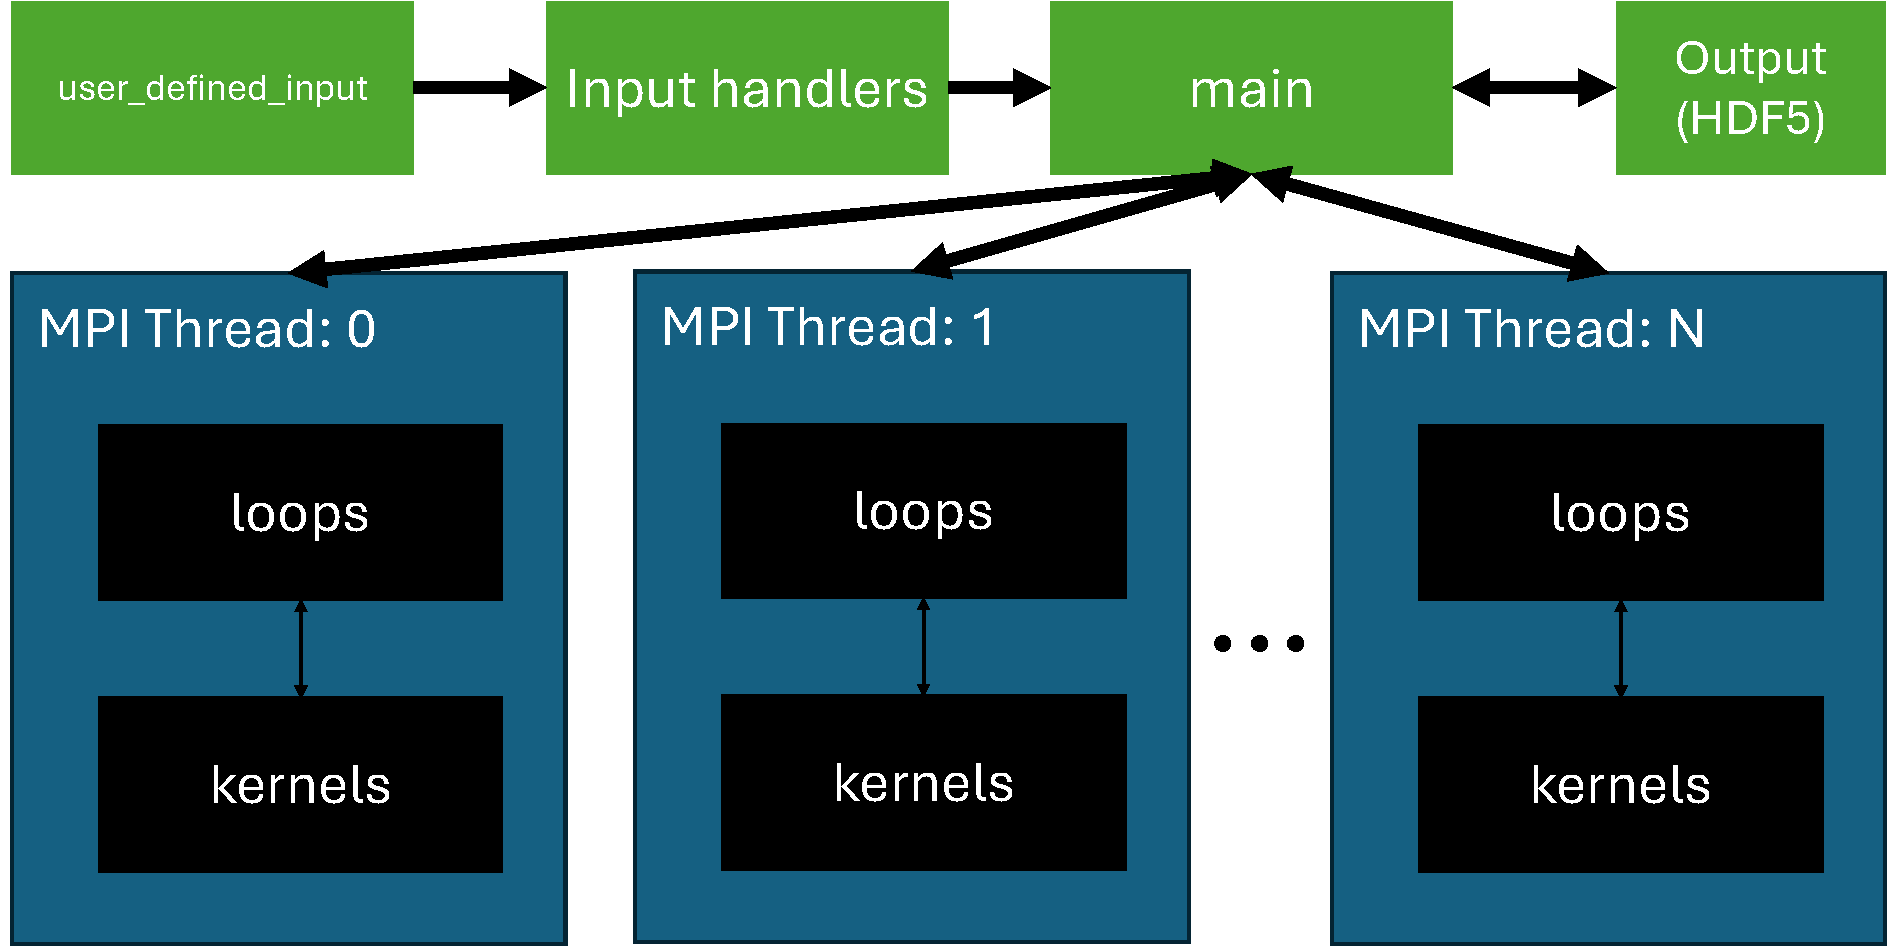
\includegraphics[width=.95\textwidth]{monte_carlo/cise_paper/cise_figs/flow.pdf}}
    \caption{MC/DC's overall structure and how functions get called and interact. Green functions are entirely Python, and black functions are compiled compute kernels if they are running in Numba CPU or GPU modes.}\vspace*{-5pt}
    \label{mpi_mcdc}
\end{figure*}

MC/DC offers a similar feature set as other Monte Carlo neutron transport applications (e.g., OpenMC \cite{romano_openmc_2015}, Shift \cite{hamilton_continuous-energy_2019}) with support for $k$-eigenvalue and fully time-dependent simulation modes in full three-dimensional constructive solid geometry.
It can model the neutron distribution in energy using either continuous energy or multigroup nuclear data.
It also supports domain decomposition.
All these features are supported on CPU (x86, ARM, POWERPC) and GPU processor targets (Nvidia and AMD), with MPI to target multiple processors (via mpi4py \cite{dalcin_mpi4py_2021}).

The number of novel schemes and simulation techniques implemented in MC/DC in a short time illustrates the success in its software engineering structure.
MC/DC supports the use of the iterative quasi-Monte Carlo (iQMC) method where deterministic and Monte Carlo transport operations run in tandem to converge solutions faster than they would in a pure Monte Carlo method. %\cite{pasmann_iqmc_nodate}
Other novel developments include global sensitivity analysis, hash-based random number generation for fully replicable solution testing, time-dependent population control, and continuously moving surfaces.
Several ongoing developments include quasi Monte Carlo, residual Monte Carlo, and machine learning techniques for dynamic node scheduling.

\section{MC/DC on CPUs}

To compile on CPUs, MC/DC uses the Numba compiler for Python to lower compute functions into LLVM and compile for a specific hardware target.
Figure~\ref{mpi_mcdc} shows MC/DC's functional layout when running in both MPI and Numba mode.

First, a user writes a Python script and imports \texttt{mcdc} as a package and forms an input script.
Then, the user interfaces with functions described in the input handler within MC/DC describing the physical models, material data, and simulation parameters.
This input layout is similar to how other Monte Carlo neutron transport applications input problems.

The input script calls a run command, which starts initialization functions within MC/DC. 
The initialization process allocates and constructs a global variable containing the user-defined inputs, meshes, particle banks, event tallies, and current global states.
This global variable is formed from a statically typed NumPy \texttt{ndarray}, which acts like a Python dictionary, where keywords are used to extract numerical arrays.
After building the global variable, initialization functions dispatch MPI processes if running in MPI mode, and begin the Monte Carlo neutron transport simulation.


Each MPI process calls functions containing the various transport algorithms and modes that MC/DC supports.
Each transport function is decorated with a Numba JIT (\texttt{@jit}) compilation flag declaring that each function must be compiled before being executed if running in Numba mode.
These transport logic loops are the highest level at which Python functions will be compiled in MC/DC.
For example, a fixed source problem will loop over all the particles and transport them until the particle's history is terminated from a physical event (e.g., capture, fission, time or space boundary), a simulation event (e.g., time census), or a variance-reduction event (e.g., population control, implicit capture).

The specific functions within each algorithm that conduct the actual transport operations (e.g., moving particles, tallying events, generating daughter particles from fission) are contained in the kernel set where all functions are \texttt{@jit} decorated.
Figure~\ref{fig:jitfunctions} shows an example compute kernel that updates the position and time of a particle as it moves.
It also shows the declaration of an \texttt{numpy.ndarray} data structure used in MC/DC.

\begin{figure}
\begin{lstlisting}[language=Python]
import numpy
from numba import jit

part = numpy.dtype([
    ('x', float64), ('y', float64),
    ('z', float64), ('ux', float64),
    ('uy', float64), ('uz', float64),
    ('v', float64) ])

@jit
def move_particle(P: part, distance):
    P['x'] += P['ux'] * distance
    P['y'] += P['uy'] * distance
    P['z'] += P['uz'] * distance
    P['t'] += distance / P['v']
\end{lstlisting}
\caption{Example of a decorated function and MC/DC's data structures based on \texttt{numpy.ndarray}.}
\label{fig:jitfunctions}
\end{figure}

After all transport is completed and the simulation is finished, the program returns to the Python interpreter and calls finalization functions.
Here, requested tally information along with statistical error provided from the Monte Carlo process are saved in an HDF5 file.
Data can be extracted from this HDF5 file and used in Python scripts to do post-processing analysis and/or data visualization with tools like Matplotlib, or post-processing can be done in other applications like Visit or Paraview.

When initially exploring a novel transport method, a developer can work in a pure Python environment where functions are entirely executed in the Python interpreter.
In this mode, the developer can bring any package into any function, do typing dynamically, and use any Python data structure.
MC/DC can be executed in MPI mode in Python as well as compiled CPU mode.
While a full Python development environment is great for initially proving a concept, it often proves to be too slow for problems of interest.

When more performance is required, developers rewrite their kernels to strictly use Numba-enabled functions.
Numba only supports a small subset of the Python ecosystem. 
Some Python data structures like dictionaries and lists can no longer be used and must instead come from NumPy implementations. 
Thus, when using Numba, the small subset of functions supported effectively becomes a domain-specific language.

Scientific computing using Python is often done with NumPy functions and data structures, making these fairly natural for numerical-methods developers to use and understand.
In fact, we have found NumPy functionality to be more commonly used in initial development than other non-supported Python methods, making the restrictions in Numba more palatable.
Some developers report skipping Python-mode development entirely and starting with Numba-CPU work for their initial proofs of concept, as they find that aids in future debugging efforts.
Similarly, other developers report making small, incremental changes in Python-based algorithms, then checking to ensure successful compilation in Numba before moving forward, roughly at every commit.
When kernels are written to support Numba mode, they can be compiled to any supported CPU targets automatically (i.e., x86, ARM64, PPC64).

We can identify pitfalls with this approach, the most significant of which are:
\begin{itemize}
    \item Common failures of \texttt{numba.object\_mode},
    \item Lack of MPI calls from within the JIT-compiled Numba code,
    \item Numba kernel debugging and profiling;
    \item Loss of functions from SciPy not implemented in NumPy, and
    \item Restrictions with \texttt{numpy.ndarray} as our primary data structure.
\end{itemize}
Most of these issues have workarounds, but make implementing numerical methods in Numba harder.

Consider that \texttt{numpy.ndarray} requires ``square'' size allocation for all elements such that the size of every named element within an array must be the same.
If one element requires \num{10000} data points and the next only \num{100}, the size of that \texttt{numpy.ndarray} is \num{20000}, which is a drastic over-allocation.
This is a primary issue for continuous energy material data, where some materials may require tens of thousands of points to fully resolve, and others may only need hundreds.
While Numba does have some features to help in this circumstance (namely experimental \texttt{jit\_classes}), we must keep the \texttt{numpy.ndarray} to support MPI calls and GPU portability.
To fix this issue, given our constraints, we are moving towards using one-dimensional vectors with length information to offset between different variables, potentially impacting MC/DC's developer-friendliness.
Accepting increased complexity to achieve portability is common in MC/DC, so developing in it can be about as difficult as in a low-level language.

Other deficiencies are known to the Numba community, and some even have ongoing open-source remedies.
For example, \texttt{numba-mpi}\footnote{\url{https://github.com/numba-mpi/numba-mpi/}} is a project to support compiled-side MPI calls, \texttt{Profila}\footnote{\url{https://github.com/pythonspeed/profila}} attempts to bring the GNU debugger to Numba kernels, and \texttt{numba-scipy}\footnote{\url{https://github.com/numba/numba-scipy}} extends support for more SciPy functions to Numba.
However, most of these community projects are still in their infancy and not robust enough to handle the large and complex structures in MC/DC.

For CPU-based HPC deployments, a Python-as-glue strategy with Numba compute kernels can enable portable (between CPU architectures and scales) and high-performance code.
However, on GPUs, if using Python+Numba alone, a developer must still have in-depth understanding of their target GPU parallelism paradigm to achieve high performance.

\section{MC/DC on GPUs}

GPUs use a single-instruction multiple-thread (SIMT) parallelism paradigm, where threads are executed in teams called warps, or wavefronts, and do the same operations in lockstep. 
If threads in the same warp need to take different paths in a program (e.g., different if/else branches or iterating loops a different number of times), each path must be executed serially.
This behavior is called thread divergence.
Threads that do not belong to the currently executing path are disabled so that the end result of the computation is consistent with the control flow logic.
Mitigating thread divergence will usually result in higher performance of GPU-enabled applications.

Unfortunately, commonly implemented Monte Carlo neutron-transport algorithms are examples of highly divergent workflows, as the behavior of any individual particle is governed by random numbers.
Much more work is often required beyond naive syntax porting to implement Monte Carlo radiation transport applications to GPUs \cite{pozulp_progress_2023}.
When compiling and running on GPUs, MC/DC uses an open-source asynchronous event scheduling library called Harmonize\footnote{\url{https://github.com/CEMeNT-PSAAP/harmonize}}~\cite{brax2023} to 
reorganize the execution of business logic and storage/movement of data to better fit the SIMT execution paradigm of GPUs.
Harmonize implements runtimes that examine operations due to be executed, segregating them into like-operations so that like-work may be executed together in batches.

Monte Carlo transport functions lend themselves to asynchronous programming schemes, as it is intuitive to provide a function for each particle operation.
For example, Figure~\ref{fig:jitfunctions} shows a \texttt{move\_particle} function.
These functions can be ordered such that like operations get implemented in unison during runtime even if user defined control logic would dictate otherwise.
The end result of the computation is the same, but the order of execution on the processor has been optimized.
MC/DC calls Harmonize via Python bindings.
Harmonize has been shown to increase GPU performance by reducing thread divergence \cite{brax2023}.


\begin{figure}
\begin{lstlisting}[language=Python]
from numba import cuda

@for_cpu
def add(array, value, idx):
    array[idx] += value

@for_gpu
def add(array, value, idx):
    cuda.atomic_add(array, value, idx)

def tally_collision_event(mcdc, part):
    id = loc2index(part)
    add(mcdc.col_tally, part.v, id)
\end{lstlisting}
\caption{Example of GPU and CPU specific API calls as defined in MC/DC and their use in a collision tally function.}
\label{fig:forcpuvgpu}

\end{figure}

% description of GPU mode execution
Moving to compile and run Numba \texttt{jit}ed functions to the GPU requires making a few alterations to the kernels themselves.
An even-smaller subset of Python functions work in GPU-compiled code, with operations supported on Numba-CPU like \texttt{numpy.linalg.solve()} losing support.
Other operations may require API-specific calls, exposed by Numba commands.
For example, atomic operations are required to preserve the side-effects of individual threads acting on global memory (e.g., adding to a tally).
To allow for a mostly unified kernel base in MC/DC for both CPUs and GPUs, we track alternate function implementations registered through decorators.

Figure~\ref{fig:forcpuvgpu} shows how we implement alternate tally accumulation functions using \texttt{@for\_cpu} and \texttt{@for\_gpu} decorators.
Here \texttt{@for\_cpu} adds one to a value in an array, and since this is within a single MPI rank we can assume a thread-safe operation.
However, on the GPU this may result in a memory race condition requiring an \texttt{numba.cuda.atomic\_add} API call.
While this does increase complexity for a programmer implementing numerical methods, it is nowhere near the complexity that might be required to accomplish a similar implementation in a compiled language.

Most numerical methods development in MC/DC is done by editing pre-existing control flow (e.g., adding more operations or device functions to existing loops, adding more components to a data structure).
Once all alterations can compile and execute using Numba-CPU functionality and necessary API calls have been abstracted, MC/DC and Harmonize automatically compile and execute those extra commands on GPUs.
So, in most cases, methods developers do not need to interface with Harmonize commands or make any alterations to the GPU runtime, data management, or compilation techniques.

If more-significant alterations are required for a given numerical method, a developer may have to interface directly with Harmonize.
We have found that, for the majority of our work exploring new algorithms to date, Harmonize+Numba sufficiently abstracts the SIMT parallelism paradigm such that operations that work on the CPU side are generally supported on GPU with little effort from the methods developer.

% descirption of compilation + harmonize
To compile functions to GPU targets with Harmonize, Numba generates intermediate compiler representations (IRs, e.g., LLVM-IR or PTX) of Monte Carlo neutron transport kernels. 
Harmonize then ingests and links those IRs with the event-scheduling runtime.
MC/DC's documentation\footnote{\url{https://mcdc.readthedocs.io/en/dev/theory/gpu.html}} provides a more in-depth description how MC/DC and Harmonize are JIT compiled for given hardware.

When running MC/DC in GPU mode on an individual MPI thread, MC/DC+Harmonize is first JIT compiled, then  during initialization allocates device memory for the global array and moves this from the host (CPU) to the device (GPU).
Next, MC/DC's transport kernels are executed with Harmonize on the GPU until transport for a given collection of work is complete.
Communication between the GPU and CPU of the global variable may be required during transport for some simulation modes.
When transport is finished, the global variable moves back to the host for a final time, and the simulation completes.
% workflow description

Just as with CPU development, this abstraction strategy has some potential disadvantages.
While MC/DC's software engineering structure allows for kernel portability between CPUs and GPUs significant time and effort can be lost in debugging, particularly for the data structures.
MC/DC only operates on GPUs using Harmonize.
Beyond its event scheduling and runtime capabilities, Harmonize allows us to ameliorate issues in Numba's GPU feature set.
For example, allocating and moving data from the CPU to GPU can only happen from Python code and cannot be done from Numba-compiled CPU kernels (requiring an \texttt{object\_mode} call).
In our initial implementations this required many copies of the global variable, which proved prohibitively costly for larger problems.
Using API calls elevated through Harmonize instead of Numba fixes this issue, requiring only two copies of the data, and the data can be accessed from both Numba-compiled CPU and GPU kernels.
In addition, when extending GPU operability to other vendors (namely AMD GPU support), Harmonize allows us to elevate non-implemented Numba API calls to the MC/DC Python interface.
For example, the Numba-HIP package\footnote{\url{https://github.com/ROCm/numba-hip}} does not currently support atomic operations on vectors.
Harmonize provides a clear path to elevate HIP-C\texttt{++} functions into Python for use in MC/DC.

For GPU development, the portability and performance enabled by MC/DC's software engineering structure increases the difficultly of implementation for the workflow developer who actually interfaces with Numba and Harmonize.
Our hope is that the investment made by the workflow developers is compounded with rapid development of more numerical methods.


\section{Performance}

\begin{figure}
    \centerline{
    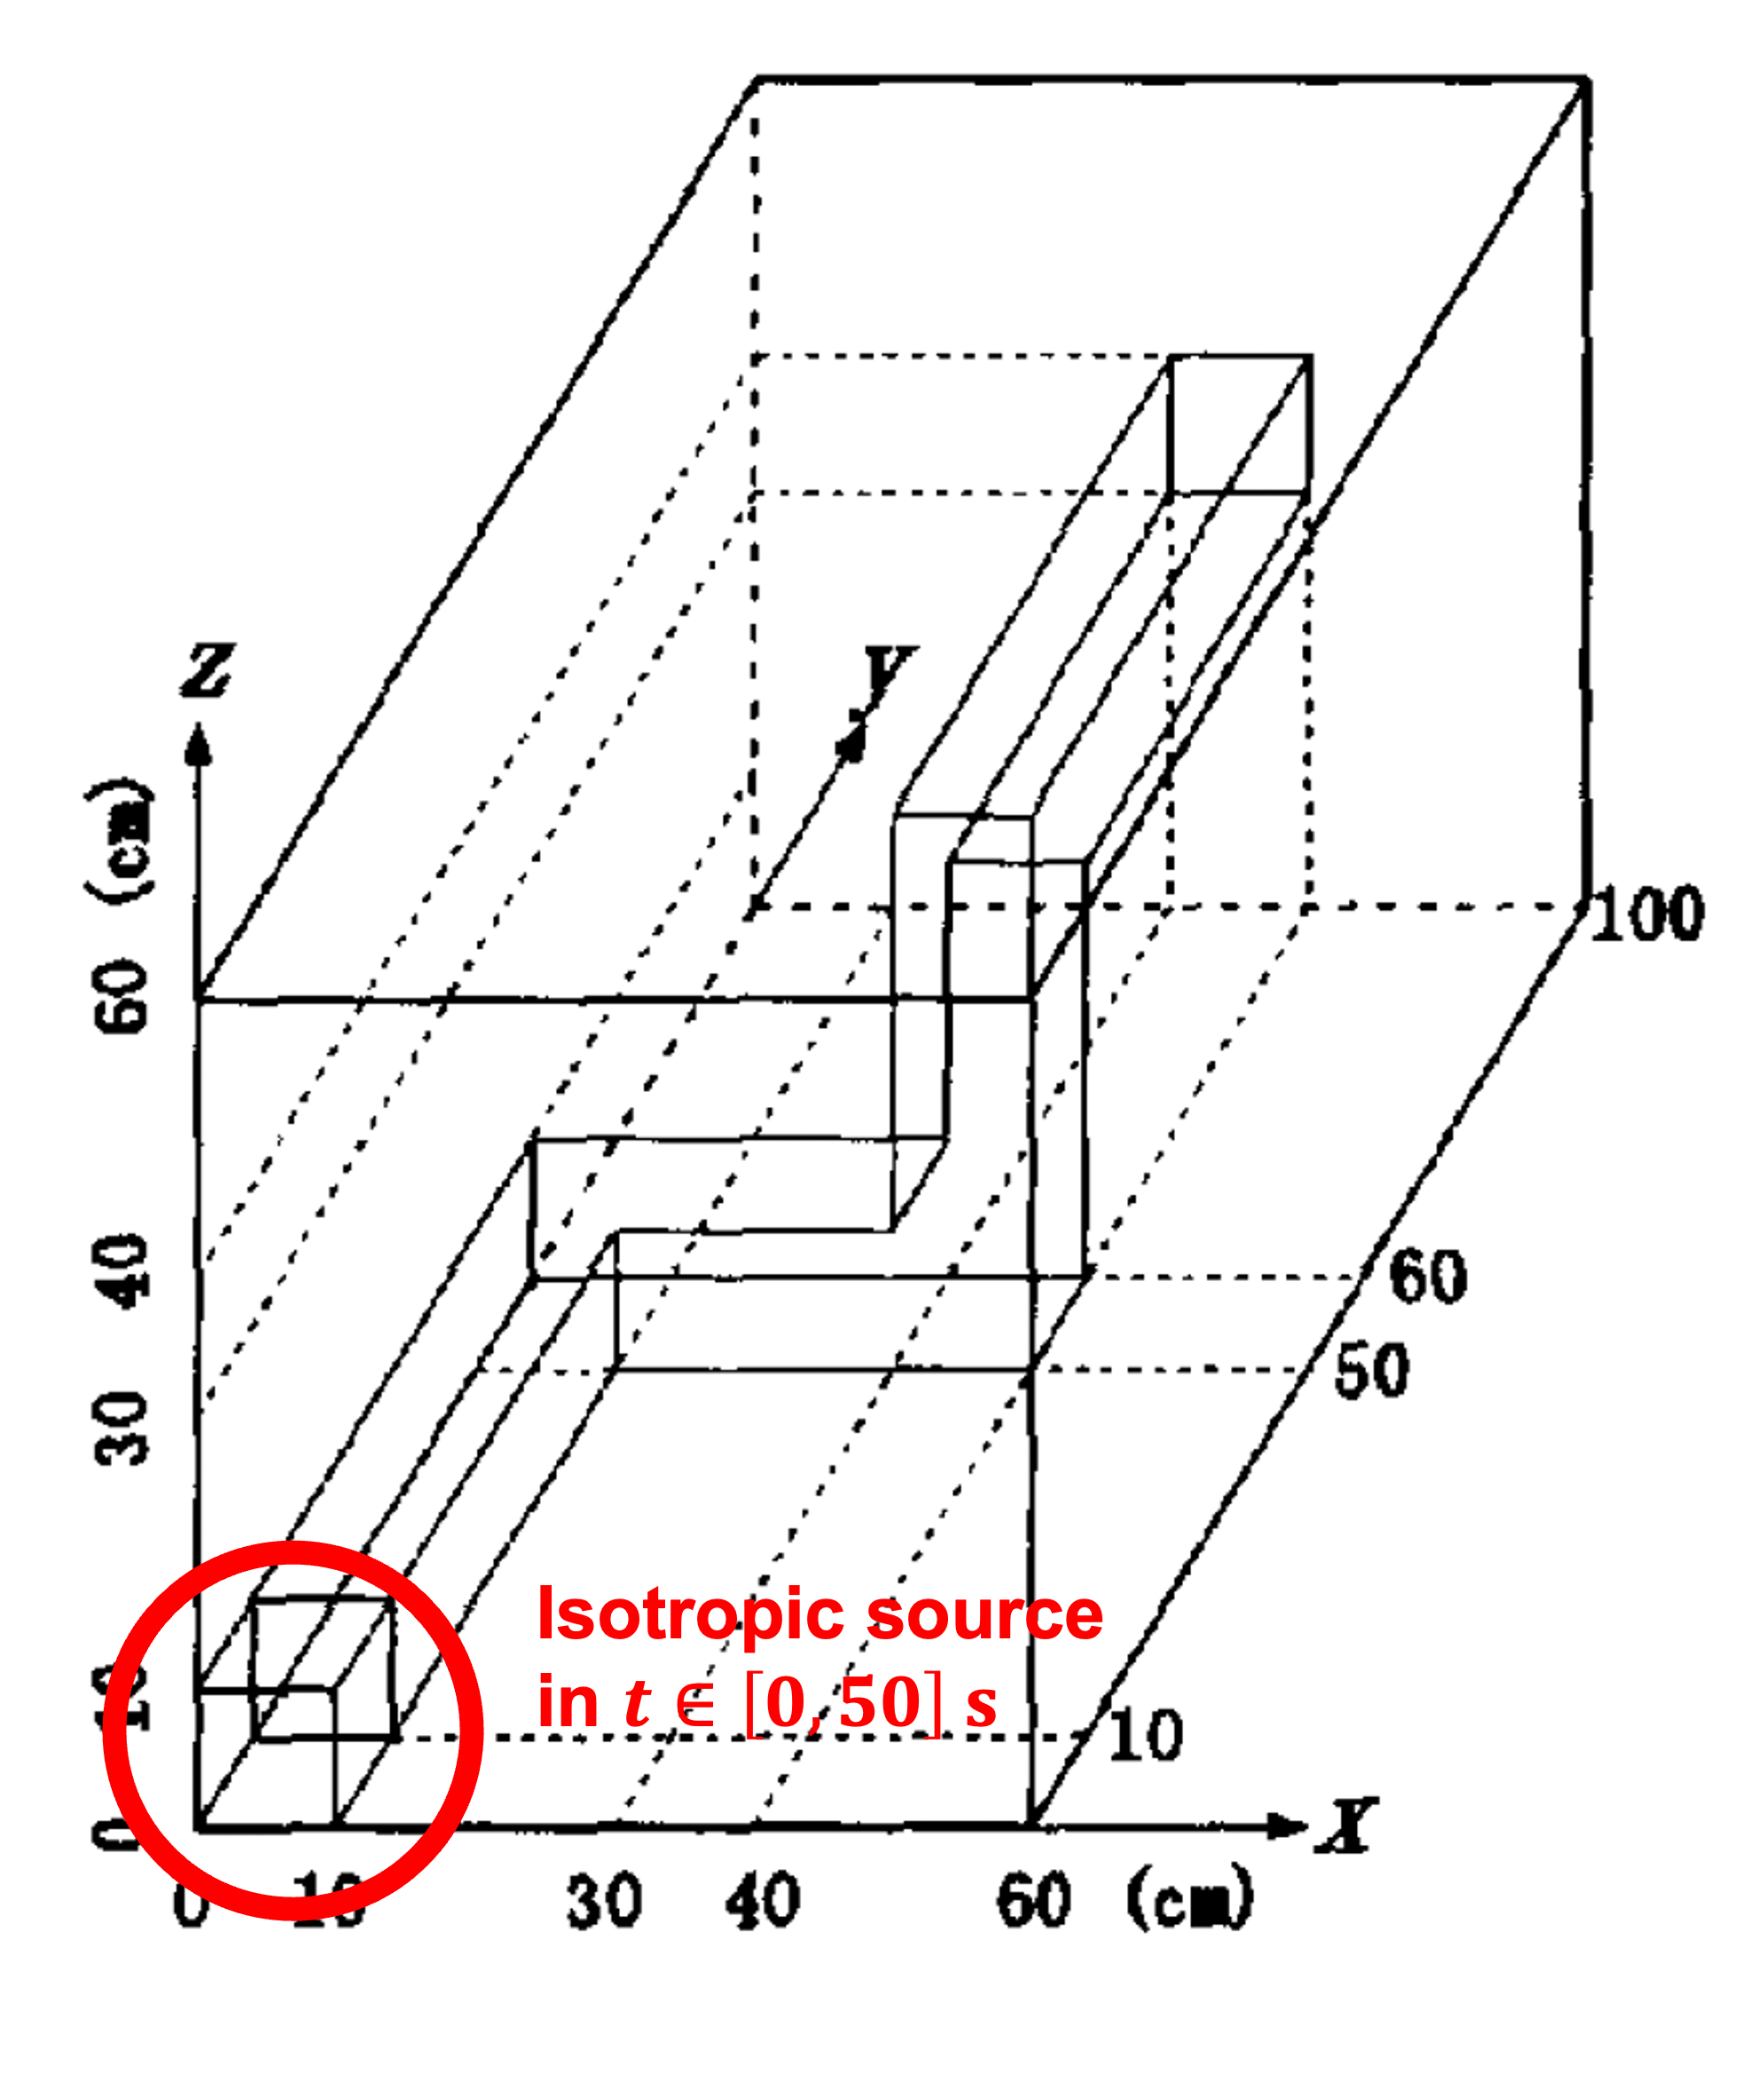
\includegraphics[width=.4 \textwidth]{monte_carlo/cise_paper/cise_figs/kobayashi_problem.png}
    } 
    \caption{Kobayashi problem schematic.}
    \label{koby-problem-def}
\end{figure}

\begin{figure*}[h]
    \centerline{
    %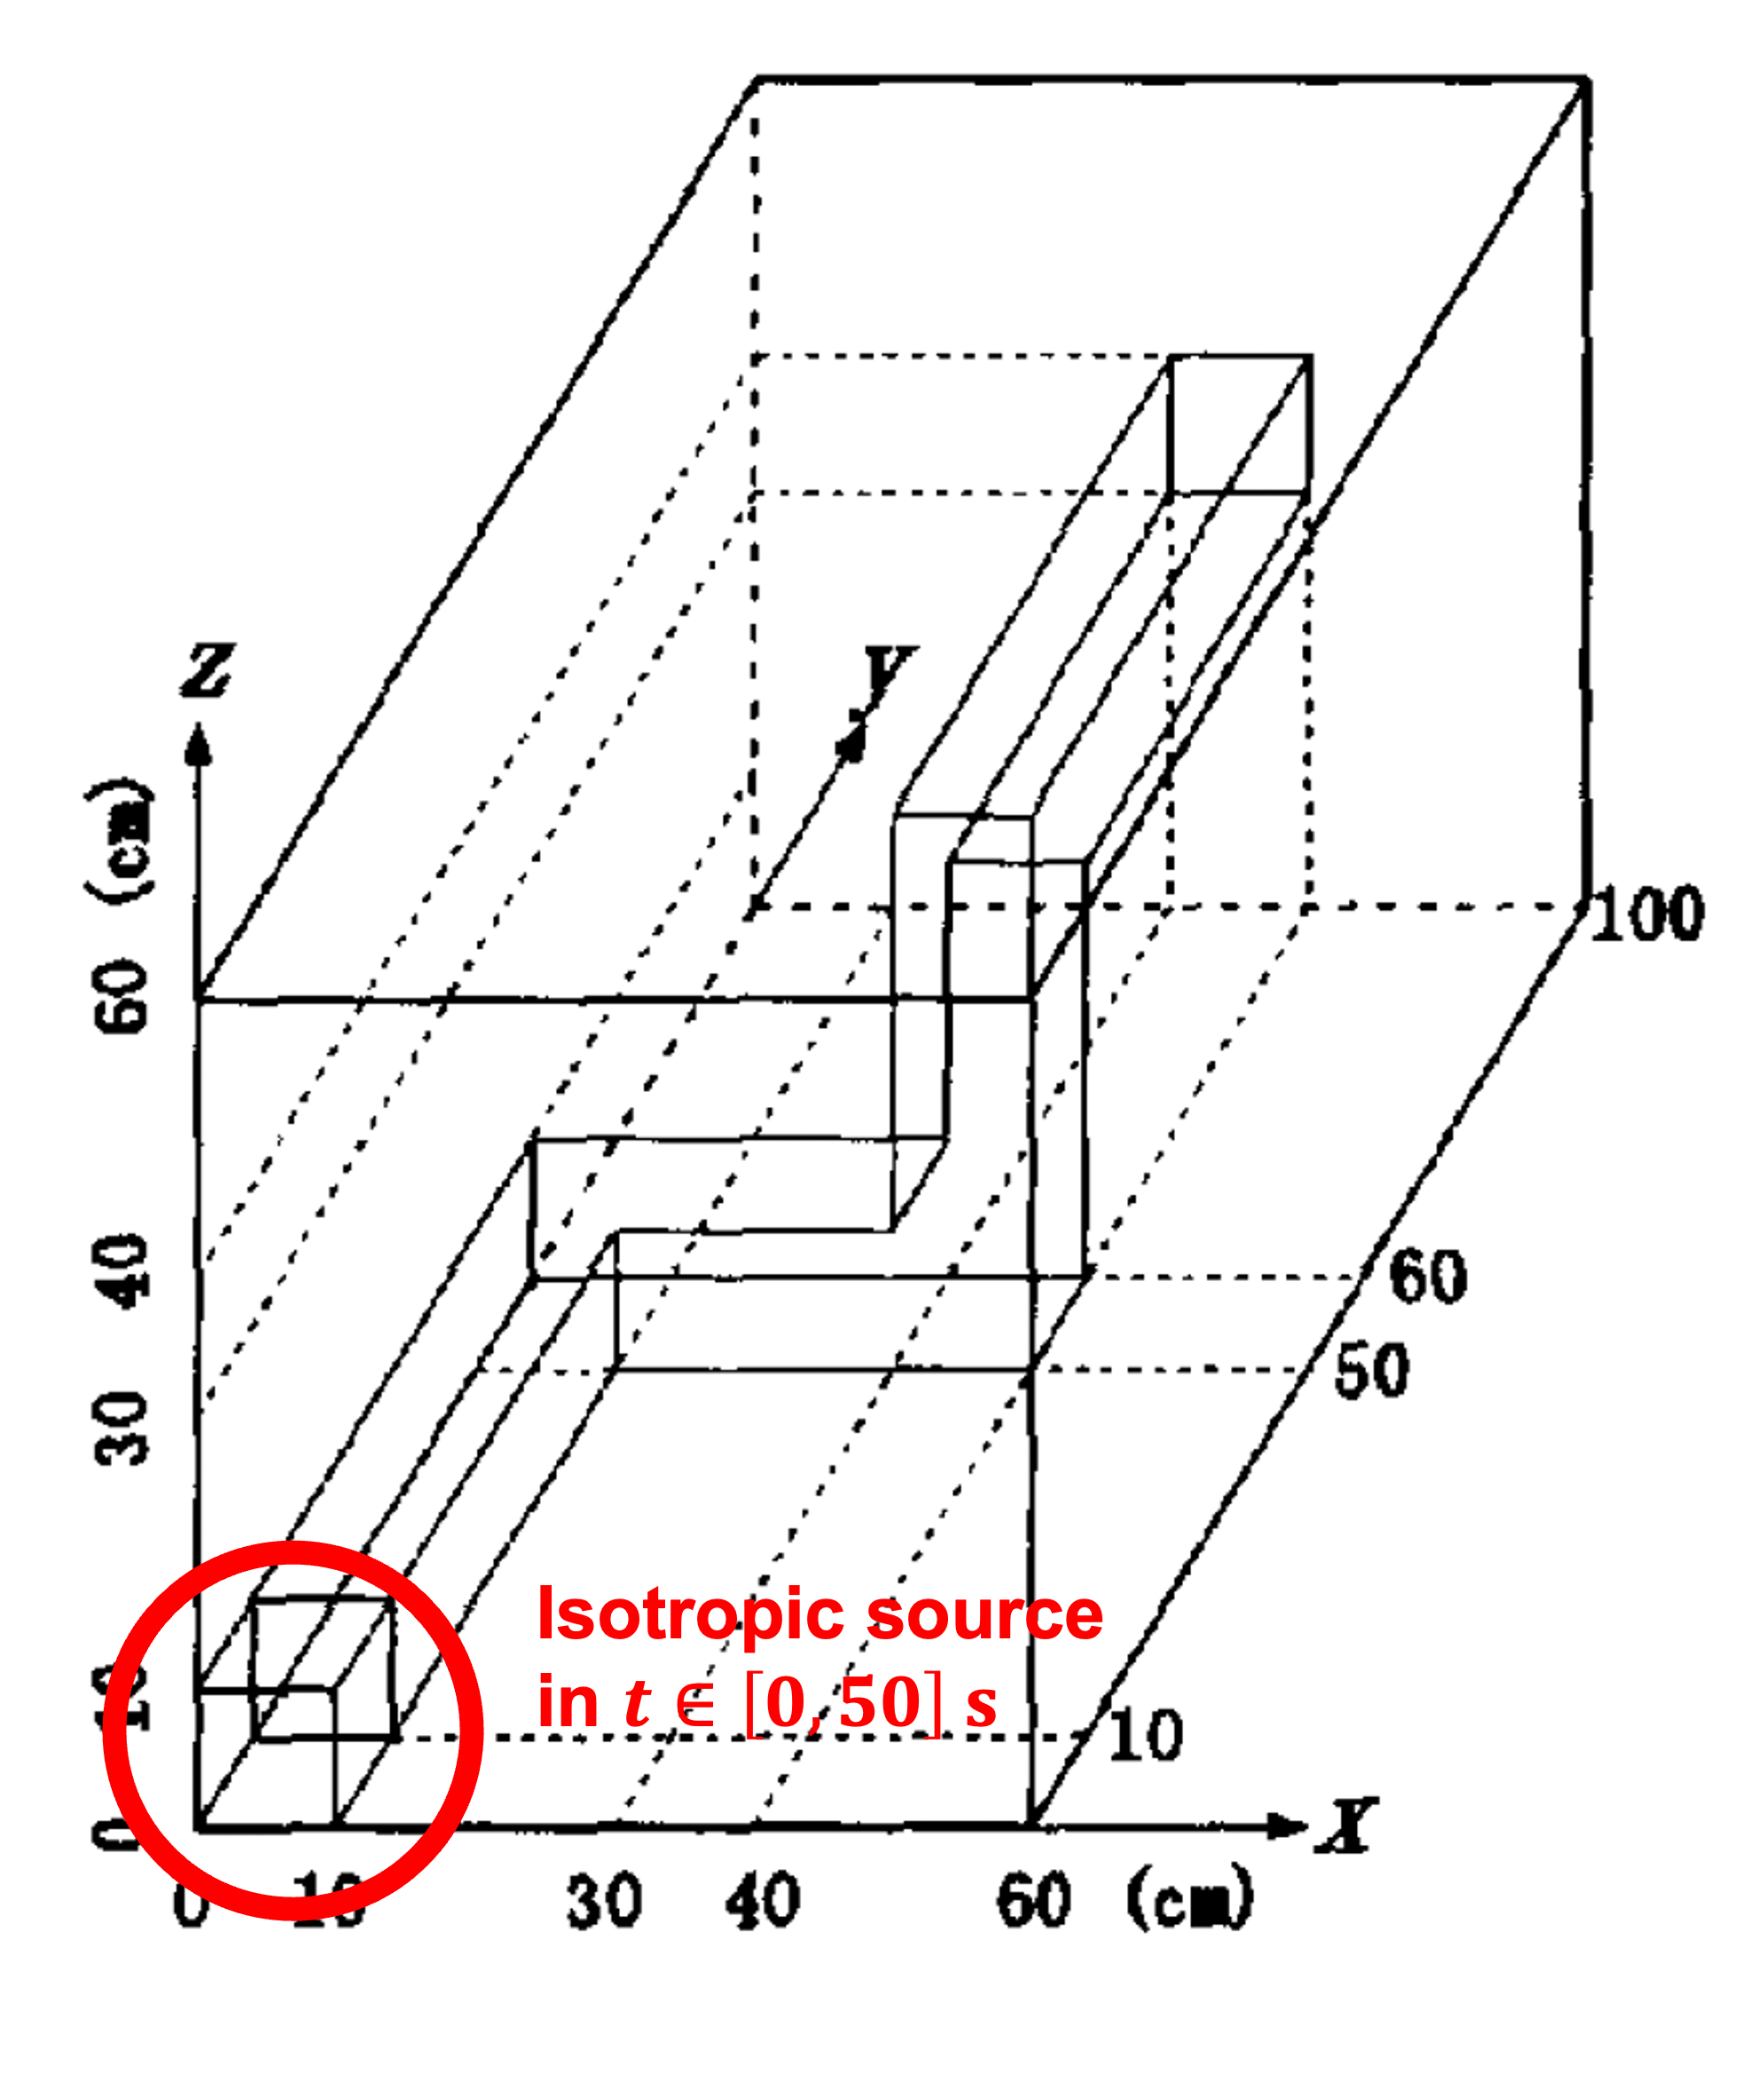
\includegraphics[width=.3\textwidth]{monte_carlo/cise_paper/cise_figs/kobayashi_problem.png} \hspace{1cm}
    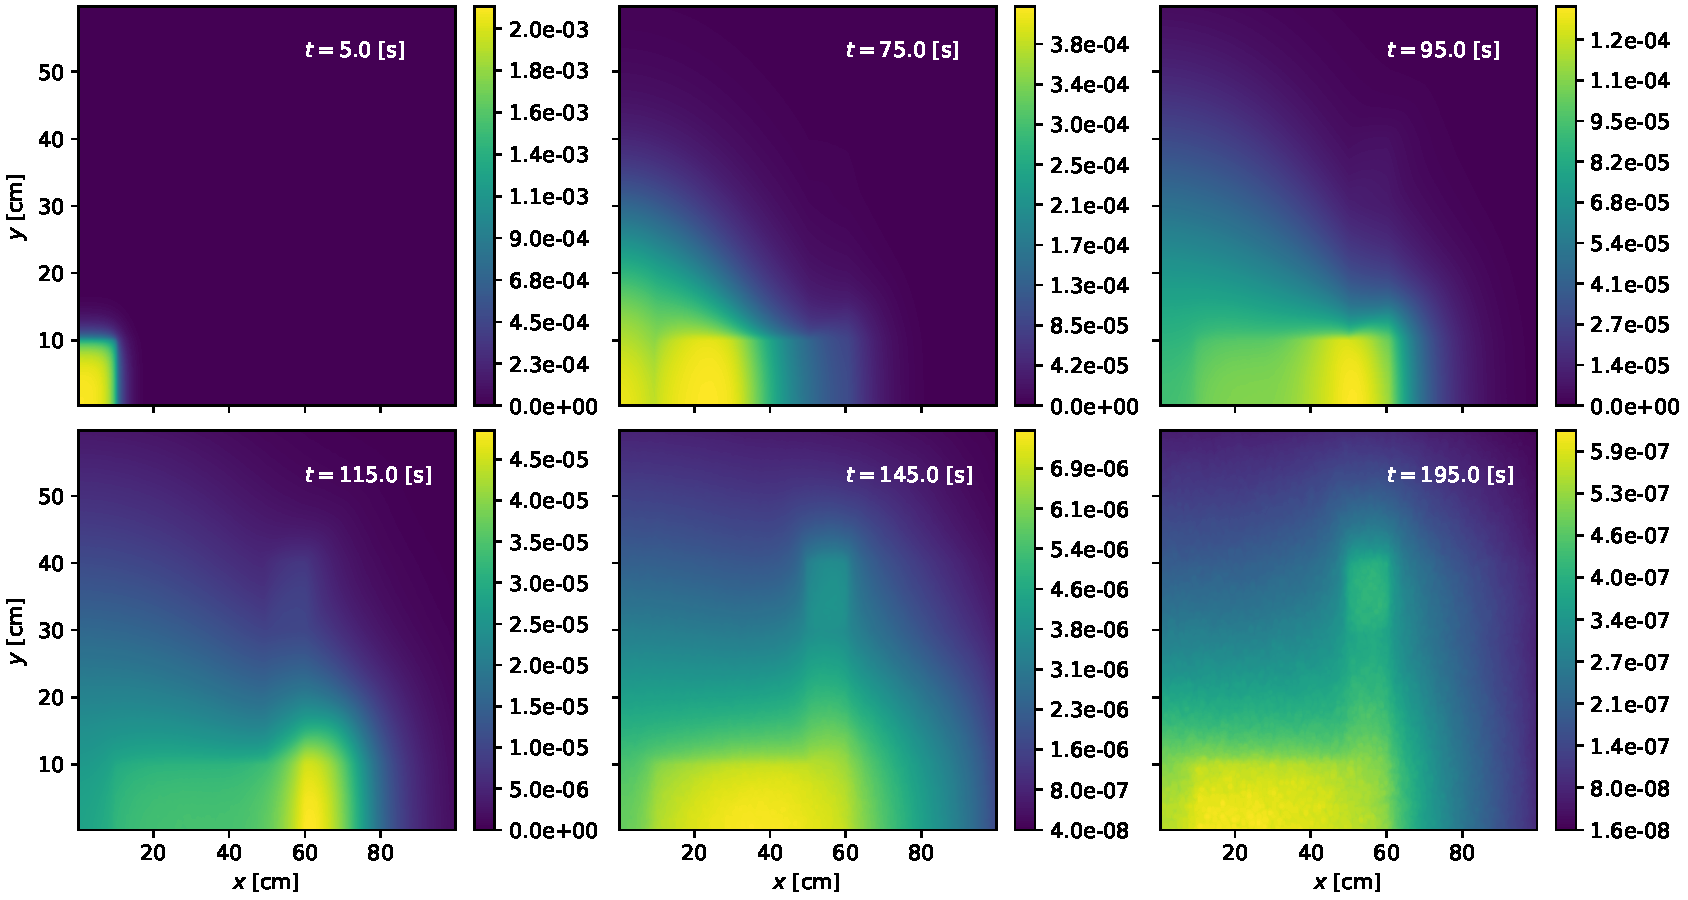
\includegraphics[width=\textwidth]{monte_carlo/cise_paper/cise_figs/koby.pdf}
    } 
    \caption{Time and space averaged scalar flux solution to the Kobayashi problem run with $1\times 10^{9}$ particle histories at various points in time.}
    \label{koby-results}
\end{figure*}

% transient runtime strong scaling mcdc v openmc maybe v shift?
To examine the performance of MC/DC we use a time-dependent version of the one-group Kobayashi dog-leg void-duct problem \cite{Kobayashi2001, variansyah_mc23_mcdc}.
Figure~\ref{koby-problem-def} shows the void duct and the location of the neutron source at the opening of the duct.
The initial condition is zero flux everywhere.
Radiation quickly moves through the void and then penetrates the walls of the problem, slowly dissipating through time.
Figure~\ref{koby-results} shows the duct clearly with the scalar flux solution at various points in time.

We solved the Kobyashi problem on HPC systems available at Lawrence Livermore National Laboratory (LLNL): the Dane and Lassen machines.
Dane is a CPU-only system with dual-socket Intel Xeon Sapphire Rapids CPUs, each with 56 cores for a total of 112 per node.
Lassen has four Nvidia Tesla V100s and two IBM Power 9 CPUs per node.
To contrast MC/DC on the CPU against a traditionally developed and compiled code, we will compare performance to another Monte Carlo neutron transport code, OpenMC\footnote{\url{https://github.com/openmc-dev/openmc}} \cite{romano_openmc_2015} (an open-source code written in C\texttt{++}).
We added time-dependent functionality to OpenMC\footnote{\url{https://github.com/CEMeNT-PSAAP/openmc/tree/transient}} so that the same algorithm is implemented in both codes for the Kobyashi problem.


Figure~\ref{performance_results} at left shows the wall-clock runtime of OpenMC (112 MPI threads), MC/DC-CPU (112 MPI threads), and MC/DC-GPU (four MPI threads) using all available resources of a given node type.
Both MC/DC runs are JIT compiled, which means compiling consumes a considerable amount of wall-clock runtime for even small problems (about \SI{70}{\s} and \SI{140}{\s} for CPU and GPU targets, respectively).
For small particle counts, actual compute time is small relative to compile time, so both MC/DC lines are flat until enough work saturates the computational power of a given resource---around \num{e8} particles for MC/DC-CPU and \num{e9} for MC/DC-GPU.
At full saturation (\num{e10} particles) MC/DC-CPU runs about 22\% slower than OpenMC, while MC/DC-GPU is 8$\times$ faster than MC/DC-CPU and 6$\times$ faster than OpenMC.

OpenMC displays superior performance at smaller particle counts due to it being a fully compiled code.
GPU profiling for MC/DC shows that
\texttt{memalloc} and \texttt{memcopy} CUDA API calls 
occupies 2.2\% of runtime (\SI{32.8}{\s} out of \SI{1500}{\s})
when running \num{e10} particles on one Lassen GPU for the Kobyashi problem.
At \num{e9} particles, GPU memory commands account for 11.8\% of runtime (\SI{18.0}{\s} out of \SI{147.0}{\s}).


Figure~\ref{performance_results} at right shows weak-scaling performance (\num{e10} particles per node) with the Kobyashi problem for MC/DC-CPU (Dane), OpenMC (Dane), and MC/DC-GPU (Lassen).
Each node is using all available compute resources for a given calculation (e.g., four nodes is 480 CPU cores and 16 GPUs on Dane and Lassen, respectively).
MC/DC-CPU shows a minimum efficiency of \num{0.85} at 256 nodes while OpenMC only falls to \num{0.89}.
OpenMC supports shared-memory parallelism (using OpenMP) but these calculations only use domain-replicated MPI.
MC/DC-GPU shows the best weak-scaling efficiency for this problem, decreasing only to \num{0.95} at 256 nodes.

\begin{figure*}[h]
    \centerline{
    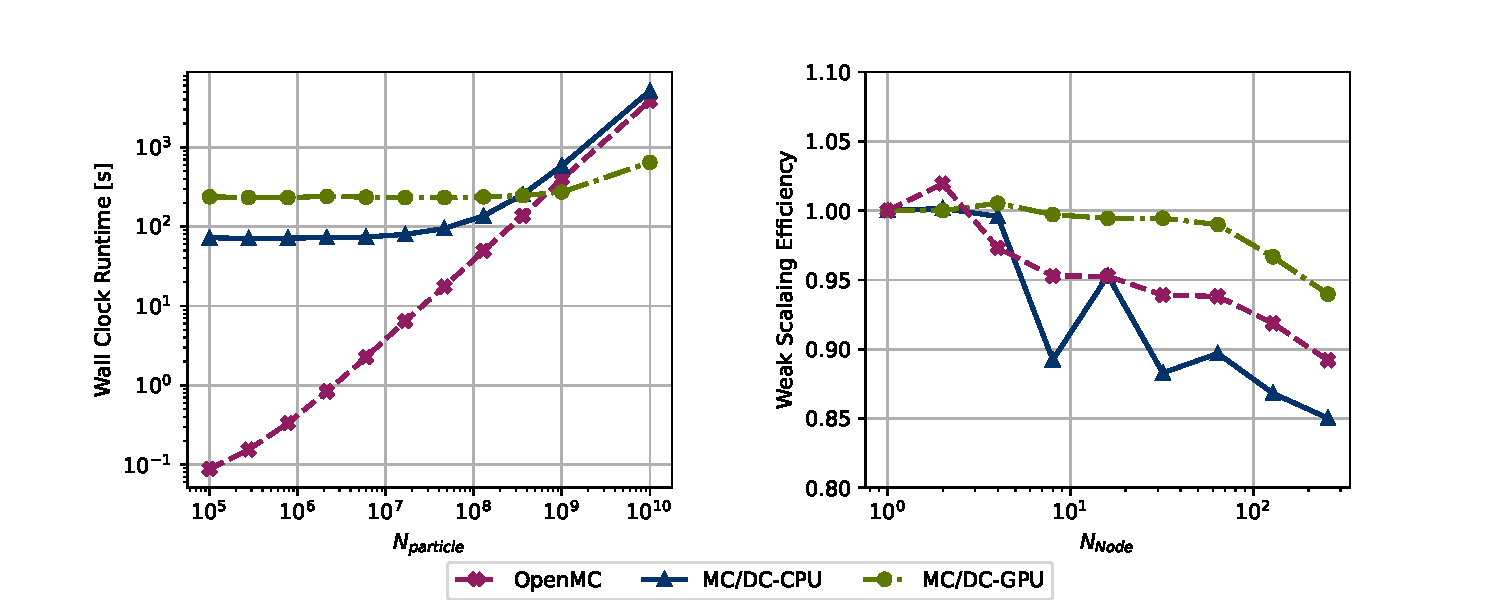
\includegraphics[width=1.1\textwidth]{monte_carlo/cise_paper/cise_figs/comps.pdf}
    }
    \caption{Left: Wall-clock runtime of the Kobyashi problem over particle counts. 
    Right: Weak scaling efficiency as a function of node count for the Kobyashi problem on Dane (CPU) and Lassen (GPU).}
    \label{performance_results}
\end{figure*}

\section{Discussion, Conclusions, and Future Work}

Monte Carlo/Dynamic Code (MC/DC) is a Monte Carlo neutron transport code that targets modern HPC architectures with CPUs and GPUs.
Our performance results demonstrate that MC/DC's structure using a Python + Numba + MPI + Harmonize scheme can produce similar performance to other Monte Carlo neutron transport solvers.
After JIT compilation overhead, MC/DC performs similarly to traditionally compiled production code on a single node for a transient problem of interest.
MC/DC exhibits similar weak scaling on CPUs and superior weak scaling on GPUs up to 256 nodes of a given HPC, compared with a CPU-only production code.

Developing using Numba for CPU targets can be as difficult as developing in low-level languages for the complicated algorithms we implement. 
This agrees with previously published analysis \cite{KailasaSrinath2022PAEi}.
We found developing the necessary time-dependent features to model the Kobyashi problem in OpenMC to be about as difficult as making changes within MC/DC.
For our application, anything gained when using a high-level-language is lost in time and effort spent circumventing unsupported operations and debugging. 
However, the implementation in OpenMC remains CPU-only, while for MC/DC it took little effort to go from a working CPU implementation to something operating and highly-performing on GPUs.
Of course, we use our own specialized event-scheduling library to do this---but Numba allows us to construct a Python-based portability framework fit to our numerical method with the added benefit of unifying our high-level glue language and kernel-production language.

Over the duration of developing MC/DC (starting in 2021) we have seen many improvements to Numba.
Compiler error reporting continues to improve (especially in Numba versions 0.59.0$+$), the number of supported operations have grown, and Numba has been extended to additional accelerators like AMD and Intel\footnote{\url{https://github.com/IntelPython/numba-dpex}} GPUs.
We have found that the Numba development team fosters a supportive community that is approachable and responsive to questions, comments, and concerns.
We believe that as Numba matures we will continue to see performance and development improvements.

Work in MC/DC is ongoing.
We are continually exploring novel variance reduction and hybrid Monte Carlo techniques, and adding new functionality.
For GPU development specifically we are currently investigating use of unified memory between the CPU and GPU as well as extending support to Intel GPUs.
We will continue to improve MC/DC, making it a portable application for rapid methods development enabled by Python and Numba.

\section{Acknowledgments}
The authors thank the Numba development team for support using the Numba compiler as well as Damon McDougall and Dominic Etienne Charrier from Advanced Micro Devices for support using Numba-HIP and ROCm compilers.
The authors thank the high performance computing staff at Lawrence Livermore National Laboratory for continued support using the Dane and Lassen machines.

This work was supported by the Center for Exascale Monte-Carlo Neutron Transport (CEMeNT) a PSAAP-III project funded by the Department of Energy, grant number: DE-NA003967.

\newpage


\printbibliography[]


% \newpage
\appendix


\chapter{Complex Spectral Radii from OCI and TDMB}
\newpage
\renewcommand{\TheTitle}{One-Cell Inversion for Solving Higher-Order Time-Dependent Radiation Transport on GPUs}
\renewcommand{\TheAuthors}{Joanna Piper Morgan,
  Travis J. Trahan,
  Timothy P. Burke,
  Colin J. Josey, 
  and Kyle E. Niemeyer}
  
\renewcommand{\TheAddress}{
    \textit{Proceedings of International Conference on Mathematics and Computational Methods Applied to Nuclear Science and Engineering (M\&C 2023)} \\
    Vol 19 2023. \\
    \doi{10.48550/arXiv.2306.07847}
}

\chapter{\TheTitle}
\label{chapter:mcatk_paper}

\PaperHeader{\TheTitle}{\TheAuthors}{\TheAddress}


\section*{Abstract}
Monte Carlo Application Toolkit (MCATK) commonly uses surface tracking on a structured mesh to compute scalar fluxes. In this mode, higher fidelity requires more mesh cells and isotopes and thus more computational overhead --- since every time a particle changes cells, new cross-sections must be found for all materials in a given cell --- even if no collision occurs in that cell. We implement a hybrid version of Woodcock (delta) tracking on this imposed mesh to alleviate the number of cross-section lookups. This algorithm computes an energy-dependent microscopic majorant cross section is computed for the problem. Each time a particle enters a new cell, rather than computing a true macroscopic cross-section over all isotopes in the cell, the microscopic majorant cross-section is simply multiplied by the total number density of the cell to obtain a macroscopic majorant cross-section for the cell. Delta tracking is then performed within that single cell. This increases performance with minimal code changes, speeding up the solve time by a factor of 1.5---1.75 for k-eigenvalue simulations and 1.2---1.6 for fixed source simulations in a series of materially complex criticality benchmarks.

\section{INTRODUCTION} 
\label{sec:mcatkintro}

The Monte Carlo Application ToolKit (MCATK) \cite{mcatk} is a Monte Carlo particle transport code that commonly uses surface tracking on a structured mesh (e.g., a Cartesian grid) to compute scalar fluxes.
The structured mesh makes distance-to-boundary calculations cheap compared to simulations using a constructive solid geometry.

Many current simulations need a great number of isotopes to be modeled properly, such that a single mesh cell might contain many isotopes. 
MCATK's standard algorithm computes the total cross-section of all isotopes in a cell every time a particle moves between cells.
Computationally expensive lookup and interpolation functions are called at every boundary crossing.
When cell sizes are small compared to a neutron mean free path, often this cross section lookup finds that a particle does not collide in the cell.
This process repeats until a collision occurs.

In this work, we introduce a hybrid-delta tracking algorithm to eliminate the macroscopic cross section lookup at surface crossings while still performing standard surface tracking.

\section{HYBRID-DELTA TRACKING}
\label{sec:mcatkmethod}

Woodcock, or delta, tracking \cite{woodcock_techniques_1965} is a variance-reduction technique that computes the majorant cross-section for the whole problem space, then uses this to determine a distance to collision for all particles.
Coupled with rejection sampling to sort for phantom collisions, and a collision estimator to compute scalar flux, delta tracking often improves performance over analogue Monte Carlo in problems that warrant it.
Many production Monte Carlo Neutron transport codes like Serpent \cite{leppanen_development_2013} use this method.

We implement a hybrid surface-delta tracking algorithm to reduce the number of cross-section lookups while still using MCATK's surface tracking on a structured mesh to find scalar flux. First we start by computing the microscopic majorant cross-section over the whole problem space, like in traditional delta tracking:
\begin{equation}
    \label{eq:majorant_mcatk}
    \sigma_{M}(E) = \max\left(\sigma_{T,k}(E), ..., \sigma_{T,K}(E)\right) \,\text{,}
\end{equation}
where $E$ is energy, $\sigma_{M}$ is the microscopic majorant cross-section, and $\sigma_{T,k}$ is the microscopic total cross-section of the $k^{\text{th}}$ material. In this work, we use one majorant over the whole problem regardless of location, but regional microscopic majorants could still be used in future work. Now to sample a distance we calculate the distance to a collision
\begin{equation}
    \label{eq:sample_mcatk}
    D = \frac{-\ln{\xi}}{N_i \sigma_{M}(E)} \, \text{,} 
\end{equation}
where $\xi$ is a random number between zero and one and $N_i$ is the number density in cell $i$.
Thus far the number density of the cell is the only parameter that depends on the particle's location in the problem, so there is no need to look up and interpolate total cross-sections when tallying the distance traveled through the mesh before a collision.
This is equivalent to assuming all atoms in the cell are of the type with the largest microscopic total cross-section at that energy.

If the potential collision occurs within the cell, we move the particle to the sampled distance and do rejection sampling, since we are now potentially forcing collisions that did not occur. We sort out these phantom collisions by allowing particles to continue to a new sampled distance if
\begin{equation}
    \label{eq:reject_mcatk}
    \xi < \frac{ \Sigma_{T,i}(E) } { N_i \sigma_M(E) } \, \text{,}
\end{equation}
where $\xi$ is a new random number between zero and one and $\Sigma_{T,i}(E)$ is the macroscopic total cross-section of the cell. 
%not sure about these indices but I want to denote that this is in a new cell and not necessarily the one next door

Since we are still moving the particles through each cell, we can use a track-length tally for estimating scalar flux.
This may not offer as much raw speed-up as full delta tracking, but may result in greater efficiency, as a track-length estimator has a lower variance than a collision estimator \cite{mc2018}.

\begin{figure}[!htb]
  \centering
  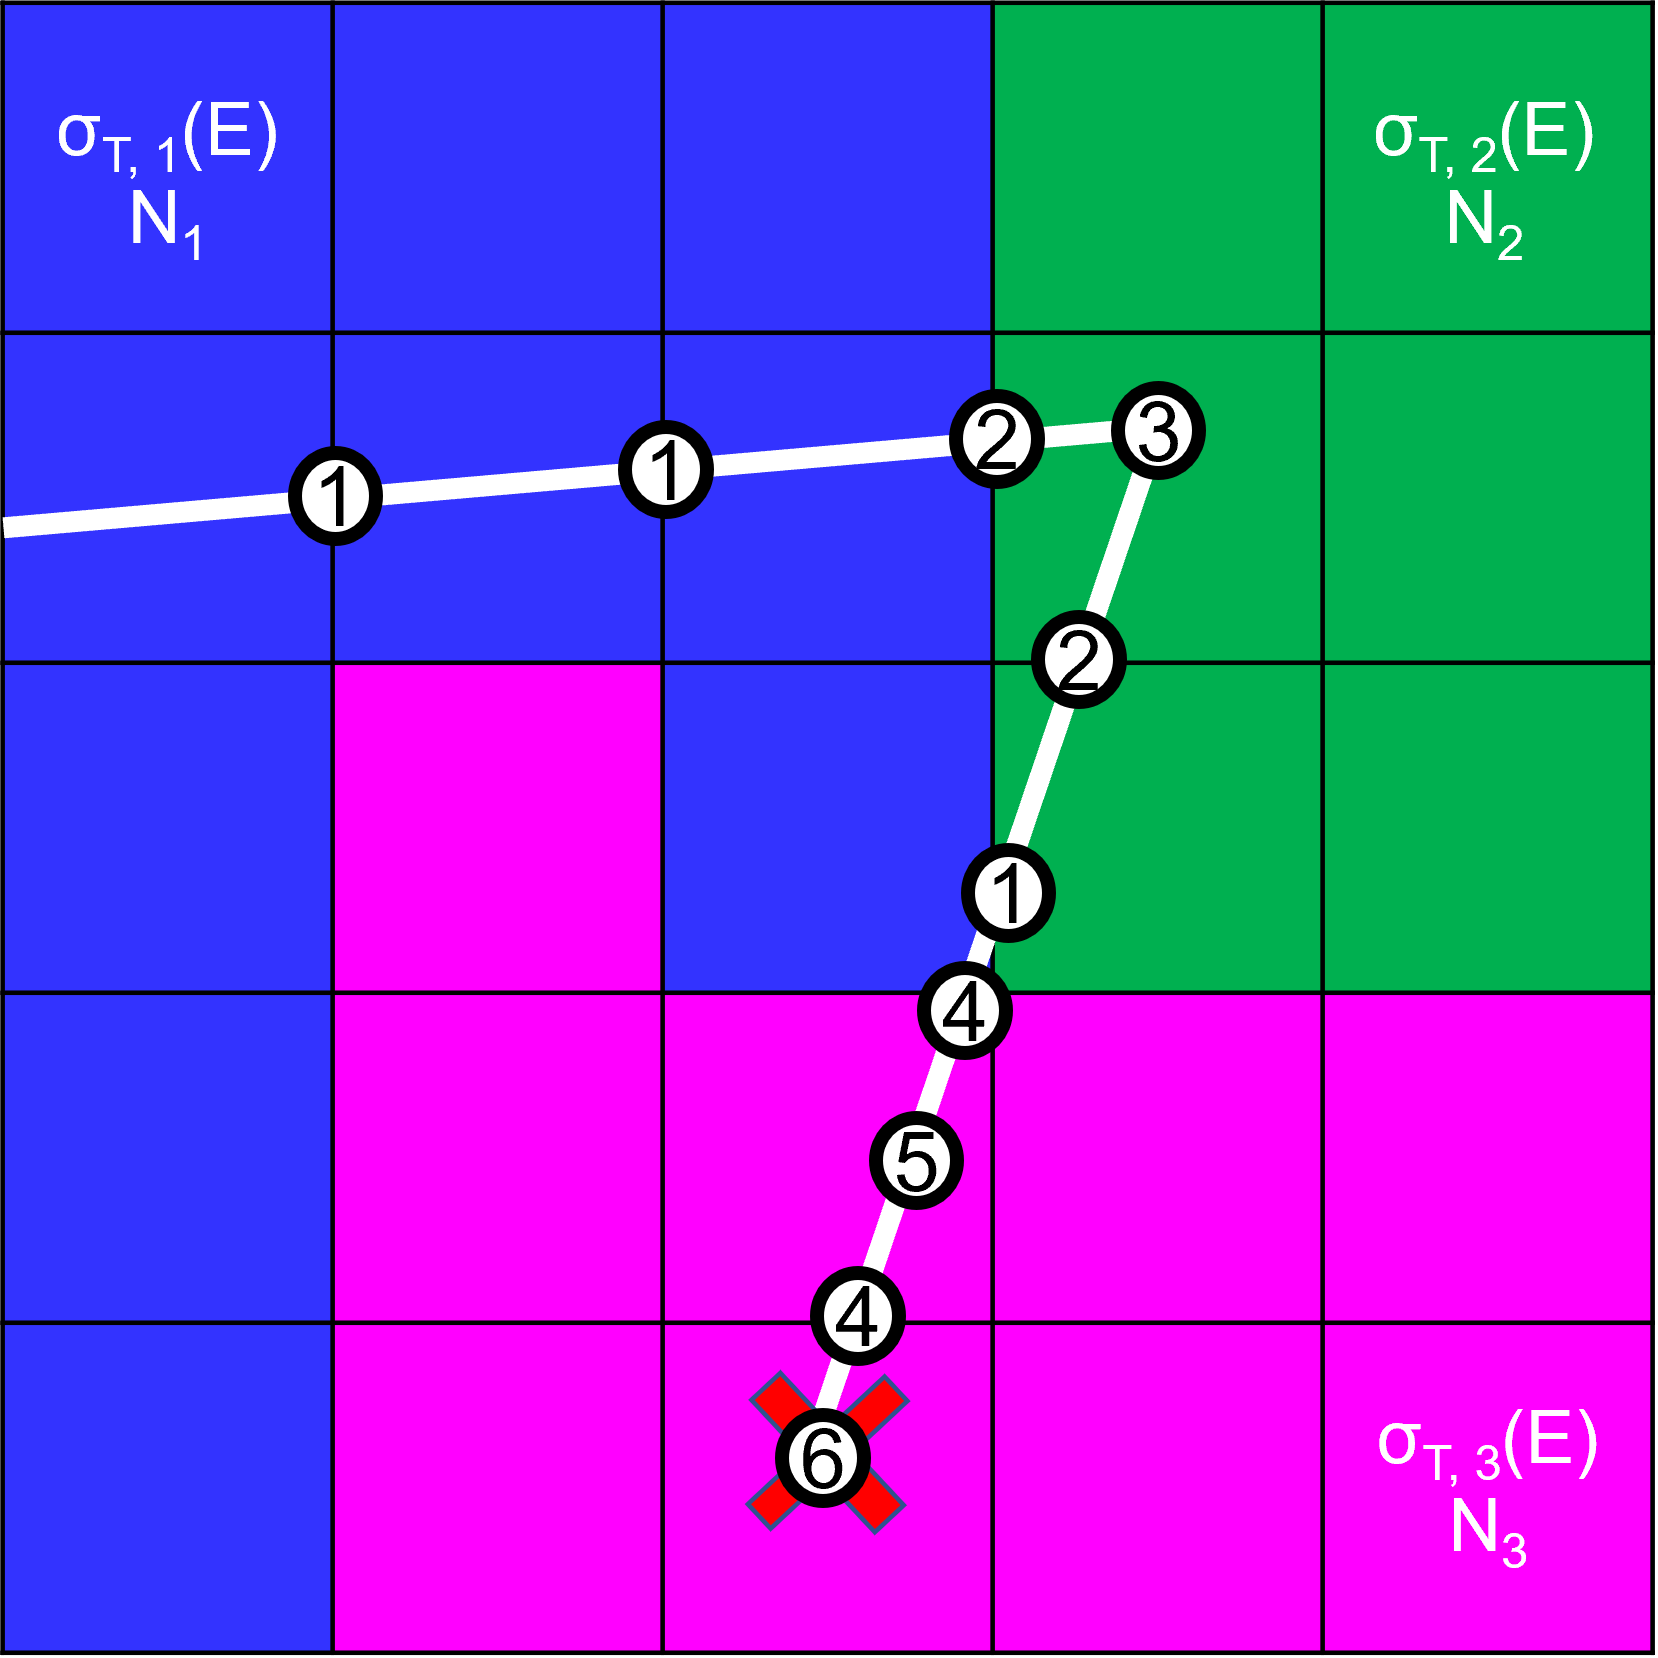
\includegraphics[scale=0.95]{appendix/mcatk_figures/algo.png}
  \caption{A material region in a structured mesh where each color represents a different material with a different ${N_i}$ and ${\sigma_T(E)}$}
  \label{fig:algo}
\end{figure}

Consider the region with three materials shown in blue, green, and pink presented in Figure \ref{fig:algo}. A particle enters the region from the left and undergoes transport with operations required at every distance to a boundary or collision:
\begin{enumerate}
    \item the particle crosses into region 1 requiring that $\sigma_M(E)$ (pre-computed) is interpolated, multiplied by $N_{1}$ to form $\Sigma_{M,1}$, and a new distance to collision is computed;
    \item the particle crosses into region 2 requiring that $\sigma_M$ (pre-computed) is interpolated then multiplied by $N_{2}$ to form $\Sigma_{M,2}$, and a new distance to collision is computed;
    \item the distance to collision is small enough to place a collision in the cell. Rejection sampling is done and it is found that this was a real event. Particle undergoes a scattering event;
    \item the particle crosses into region 3 requiring that $\sigma_M$ (pre-computed) is interpolated then multiplied by $N_{3}$ to form $\Sigma_{M,3}$, and a new distance to collision is computed;
    \item the distance to collision  is small enough to place a collision in the cell. A potential collision is rejected; and
    \item the distance to collision  is small enough to place a collision in the cell. Rejection sampling determines that the collision is real, and the particle is absorbed.
\end{enumerate}
Here, $\sigma_M = \max{(\sigma_{T,1}, \sigma_{T,2}, \sigma_{T,3})}$. $\sigma_{T,i}$ is only looked up for rejection sampling, required in operations 3, 5 and 6. For this hypothetical problem we have reduced the number of lookups to find $\sigma_{T,i}$ from ten to three. Depending on the number of isotopes in the cell, this could represent a significant number of operations.
Speed-up in MCATK with this method comes from the avoidance of these lookup functions to find the dominant total microscopic cross section between \textit{all} the isotopes that are contained within a cell. 
We expect a significant speed-up as this function is called frequently in standard surface tracking. 
We also expect that the speedup will be greater when there are more isotopes within a cell. 
All other operations remain the same between standard tracking and hybrid surface-delta tracking on the structured mesh.

Extending our implementation of the hybrid-delta tracking scheme in models that use constructive solid geometry instead of structured meshes will require no additional work.
Since small cell sizes in structured meshes is analogous to complex and small geometries in constructive solid geometry, we expect similar performance increases when these models also have complex isotopic compositions.

We first implemented hybrid-delta tracking in MCATK's k-eigenvalue algorithm then implemented it for fixed source problems.
Since all of MCATK's algorithms (e.g., k-eigenvalue, fixed source, etc.) use the same collision kernel no alterations were required to move from an implementation in one algorithm to the next other than Boolean switches to initialize the mini-delta tracking algorithm.


\section{BENCHMARKS}
\label{sec:mcatkbenchmarks}
We investigated the performance of hybrid-delta tracking on a series of benchmark problems: one from the Godiva IV experiment (HEU-MET-FAST-086, case 5) and two from the MUSiC experiment.
All three are materially complex, having between 48 and 125 isotopes over the whole model, and implement a structured tracking mesh imposed on the geometry. 
The minimum mesh cell dimension is 1 mm in the fissile region of each problem.

%\subsection{Godiva IV}
%\label{subsec:godiva}
The Godiva IV super-prompt-critical burst experiments use two control rods and one burst rod made of highly enriched uranium and molybdenum to control criticality \cite{osti_9564352009}.
As the rods are inserted reactivity goes up, and vice versa when they are removed.
The only fission source is the spontaneous fission from the highly enriched uranium in the experiment.
Figure \ref{fig:godiva} shows a cross section of the Godiva IV core assembly and restraints which are modeled in our benchmark.
This is the simplest benchmark we model, requiring the fewest number of isotopes. 

\begin{figure}[!htb]
  \centering
  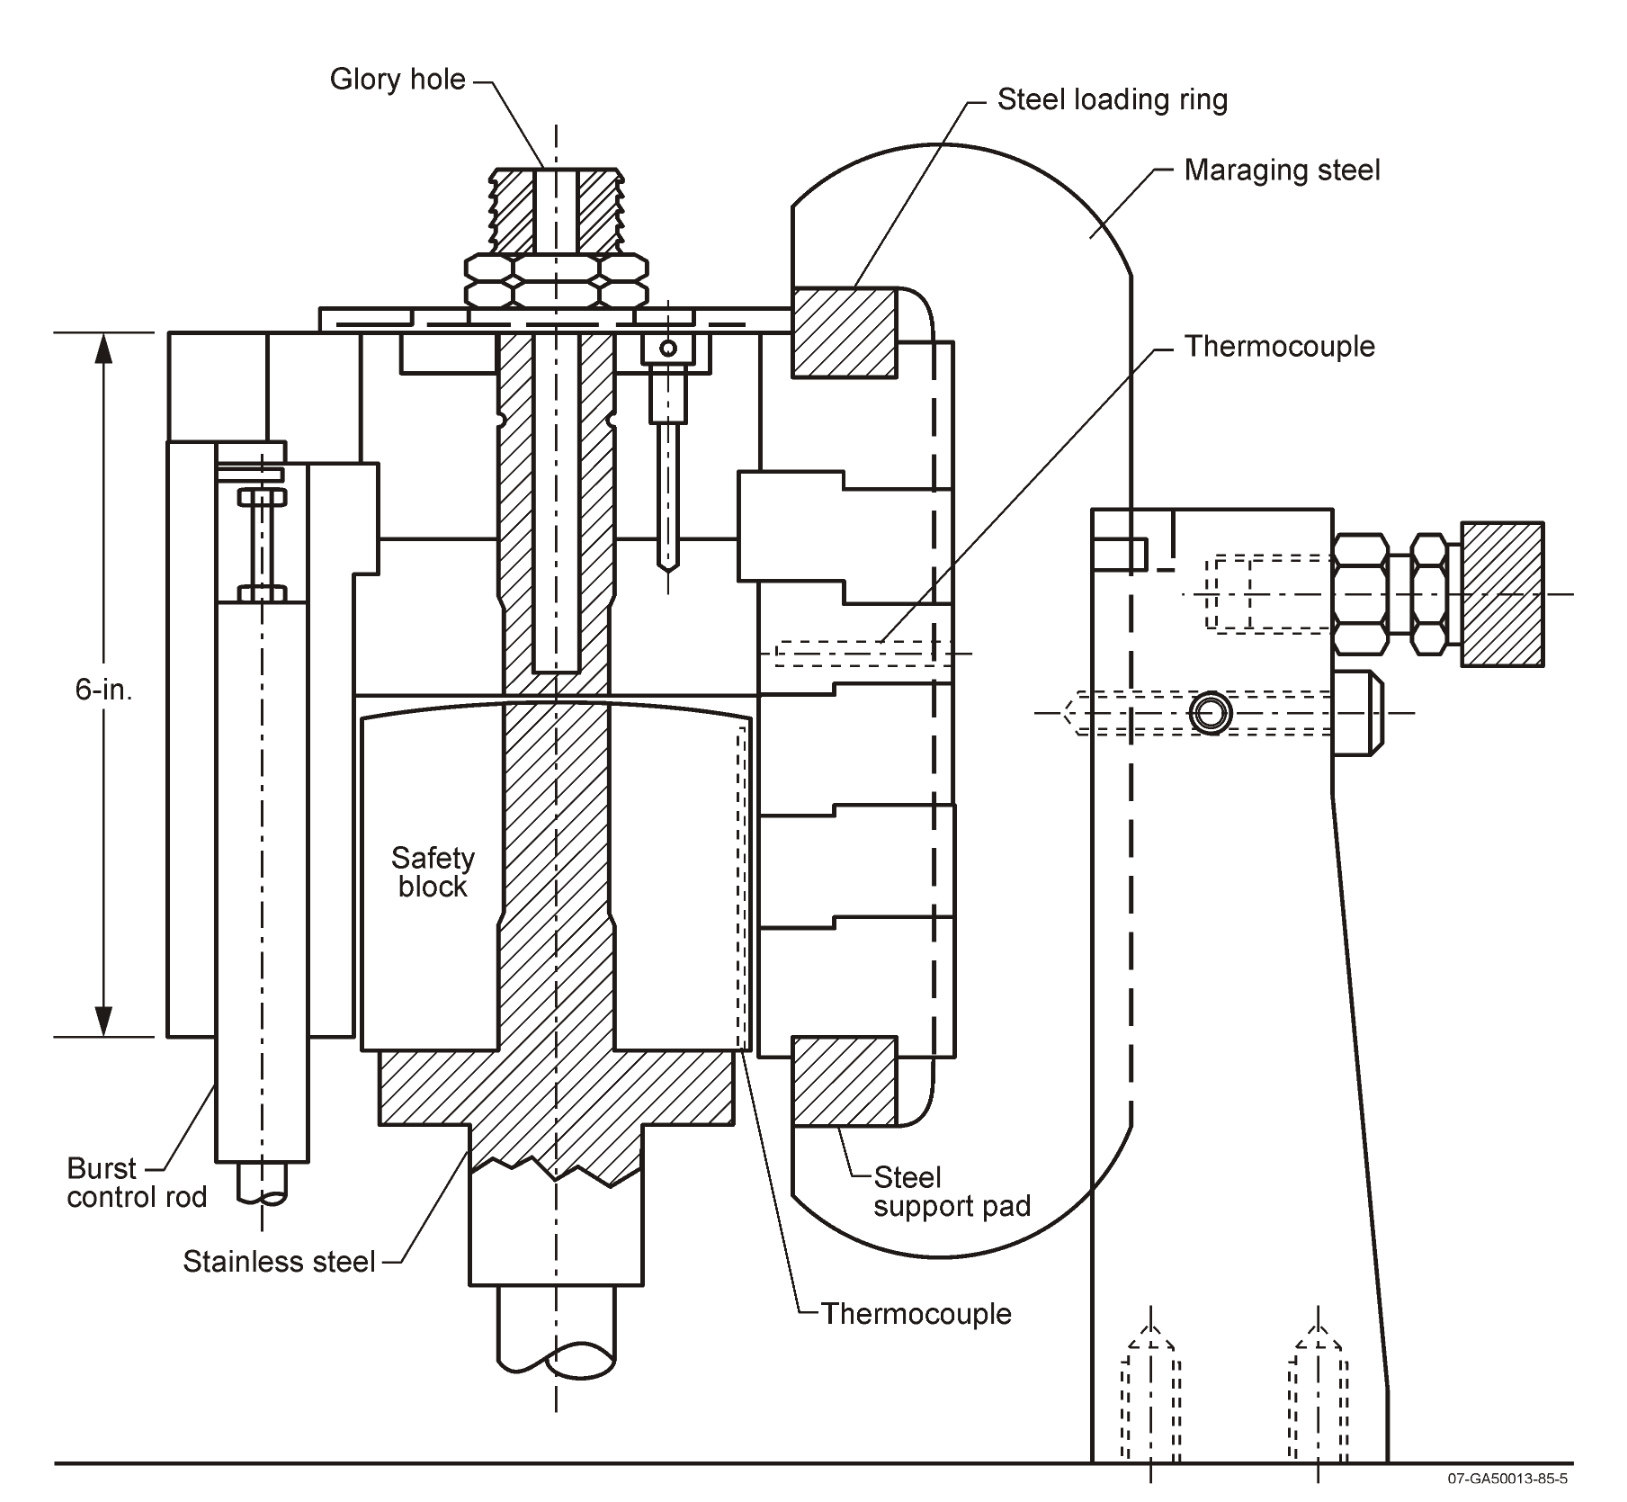
\includegraphics[scale=0.6]{appendix/mcatk_figures/godivaIV.PNG}
  \caption{Cutaway view of the Godiva IV core and its restraints used in the HEU-MET-FAST-086 benchmark \cite{godiva2014}. }
  \label{fig:godiva}
\end{figure}

%\subsection{MUSiC}
%\label{subsec:music}

The Measurement of Uranium Subcritical and Critical (MUSiC) experiments (IER 488) use stack-able hemispheres of highly enriched uranium --- known as the Rocky Flats Shells --- to take data with various detectors \cite{music2021}.
Figure \ref{fig:music} at right shows the highly enriched uranium shells which are about \SI{0.3}{\centi\meter} thick and have variable radii between about \SI{2}{\centi\meter} and \SI{10}{\centi\meter}.
Figure \ref{fig:music} at left shows the full configuration of the experiment with fission sources and detectors.
Fission is induced with a Cf-252 source at the center of the shell array as well as an external deuterium source.

\begin{figure}[!htb]
  \centering
  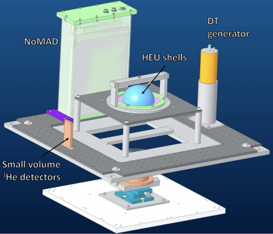
\includegraphics[width=0.39\textwidth]{appendix/mcatk_figures/MUSiC/music_config.png}
  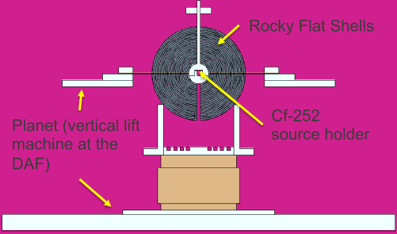
\includegraphics[width=0.57\textwidth]{appendix/mcatk_figures/MUSiC/rocky_flats.png}
  \caption{Left: Overall configuration of the MUSiC experiment. Right: Schematic of the Rocky Flats highly enriched uranium hemispherical shells \cite{osti_1781360} }
  \label{fig:music}
\end{figure}

\section{PERFORMANCE RESULTS} 
\label{sec:mcatkresults}

We verified all models on both k-eigenvalue and fixed source problems with the standard tracking algorithm from MCATK, then computed the speed-up from our hybrid-delta tracking scheme.
To produce timing results these benchmarks ran with 1 rank; however, parallelization is already enabled for hybrid-delta tracking in MCATK via MPI.
Material, geometry, and mesh between k-eigenvalue and fixed source simulations are the same for a given case.

\subsection{k-eigenvalue Simulation}
K-eigenvalue simulations were started with 100 inactive cycles before 500 active ones using \num{1e5} particles in each cycle.
Table \ref{table:mcatkruntime} shows the performance increase when hybrid-delta tracking is enabled.
The differences in eigenvalue between simulations with and without the hybrid-delta tracking algorithm are all within 1.12 standard deviations. This table also shows a significant speed-up in the over all solve time of MCATK with delta tracking incurring between a 1.54 --- 1.75$\times$ speed-up.

\begin{table}[!htb]
  \centering
  \caption{Benchmark results: where ${\Delta \sigma}$ is the difference in number of standard deviations of ${k_{\text{eff}}}$ between the standard algorithm and hybrid-delta tracking.}
  \label{table:mcatkruntime} 
  \begin{tabular}{c c c c c c  } \hline 
    Test Model & MCATK & MCATK & $k$ & $\Delta \sigma$ & speed-up\\
               & Surface (s)  & Hybrid-Delta (s) &  & &\\ \hline
    \ Godiva Case 5 & 16900 &  10987 & 0.99736 &  -0.747 & 1.54 \\
    \ MUSiC Case 8  & 23937 &  14832 & 0.99970 &  0.130 & 1.61 \\
    \ MUSiC Case 9  & 22649 &  12973 & 0.99929 &  -1.105 & 1.75 \\ 
    \hline
  \end{tabular}
\end{table}

\subsection{Fixed Source Simulations}

To compute error between tracking schemes in fixed source simulations we used the estimates of the $\alpha$-eigenvalue computed using MCATK's time-dependent algorithm.
The benchmarks were started at \SI{0}{\second} and ran to \SI{500e-8}{\second} with a time step of $\Delta t =$ \SI{1e-8}{\second}.
The particle population was combed between every time step up or down to \num{1e5} particles. 
Table \ref{table:runtime_trans} shows less speed-up then for k-eigenvalue computations (only between 1.24$\times$ and 1.63$\times$) but still significant for minimal alterations to a production code. This table also shows the average $\alpha$-eigenvalues method within three standard deviations.

\begin{table}[!htb]
  \centering
  \caption{ Benchmark results: where ${\Delta \sigma}$ is the difference in number of standard deviations of the $\alpha$-eigenvalues between standard algorithm and hybrid-delta tracking.}
  \label{table:runtime_trans} 
  \begin{tabular}{c c c c c c } \hline 
    Benchmark & MCATK            & MCATK         & $\alpha_{\text{avg}}$ & $\Delta \sigma$ & speed-up\\
               & Surface (s)  & Hybrid-Delta (s) & &                 &\\ \hline
    \ Godiva Case 5 & 2689 &  2168 & \num{-3.54e-3} &  \num{-1.91} & 1.24 \\
    \ MUSiC Case 8  & 4352 &  2665 & \num{-1.26e-3} &  \num{-0.76} & 1.63 \\
    \ MUSiC Case 9  & 4440 &  2786 & \num{-1.02e-3} &  \num{-2.75} & 1.59 \\ 
    \hline
  \end{tabular}
\end{table}

\begin{figure}[!p]
  \centering
  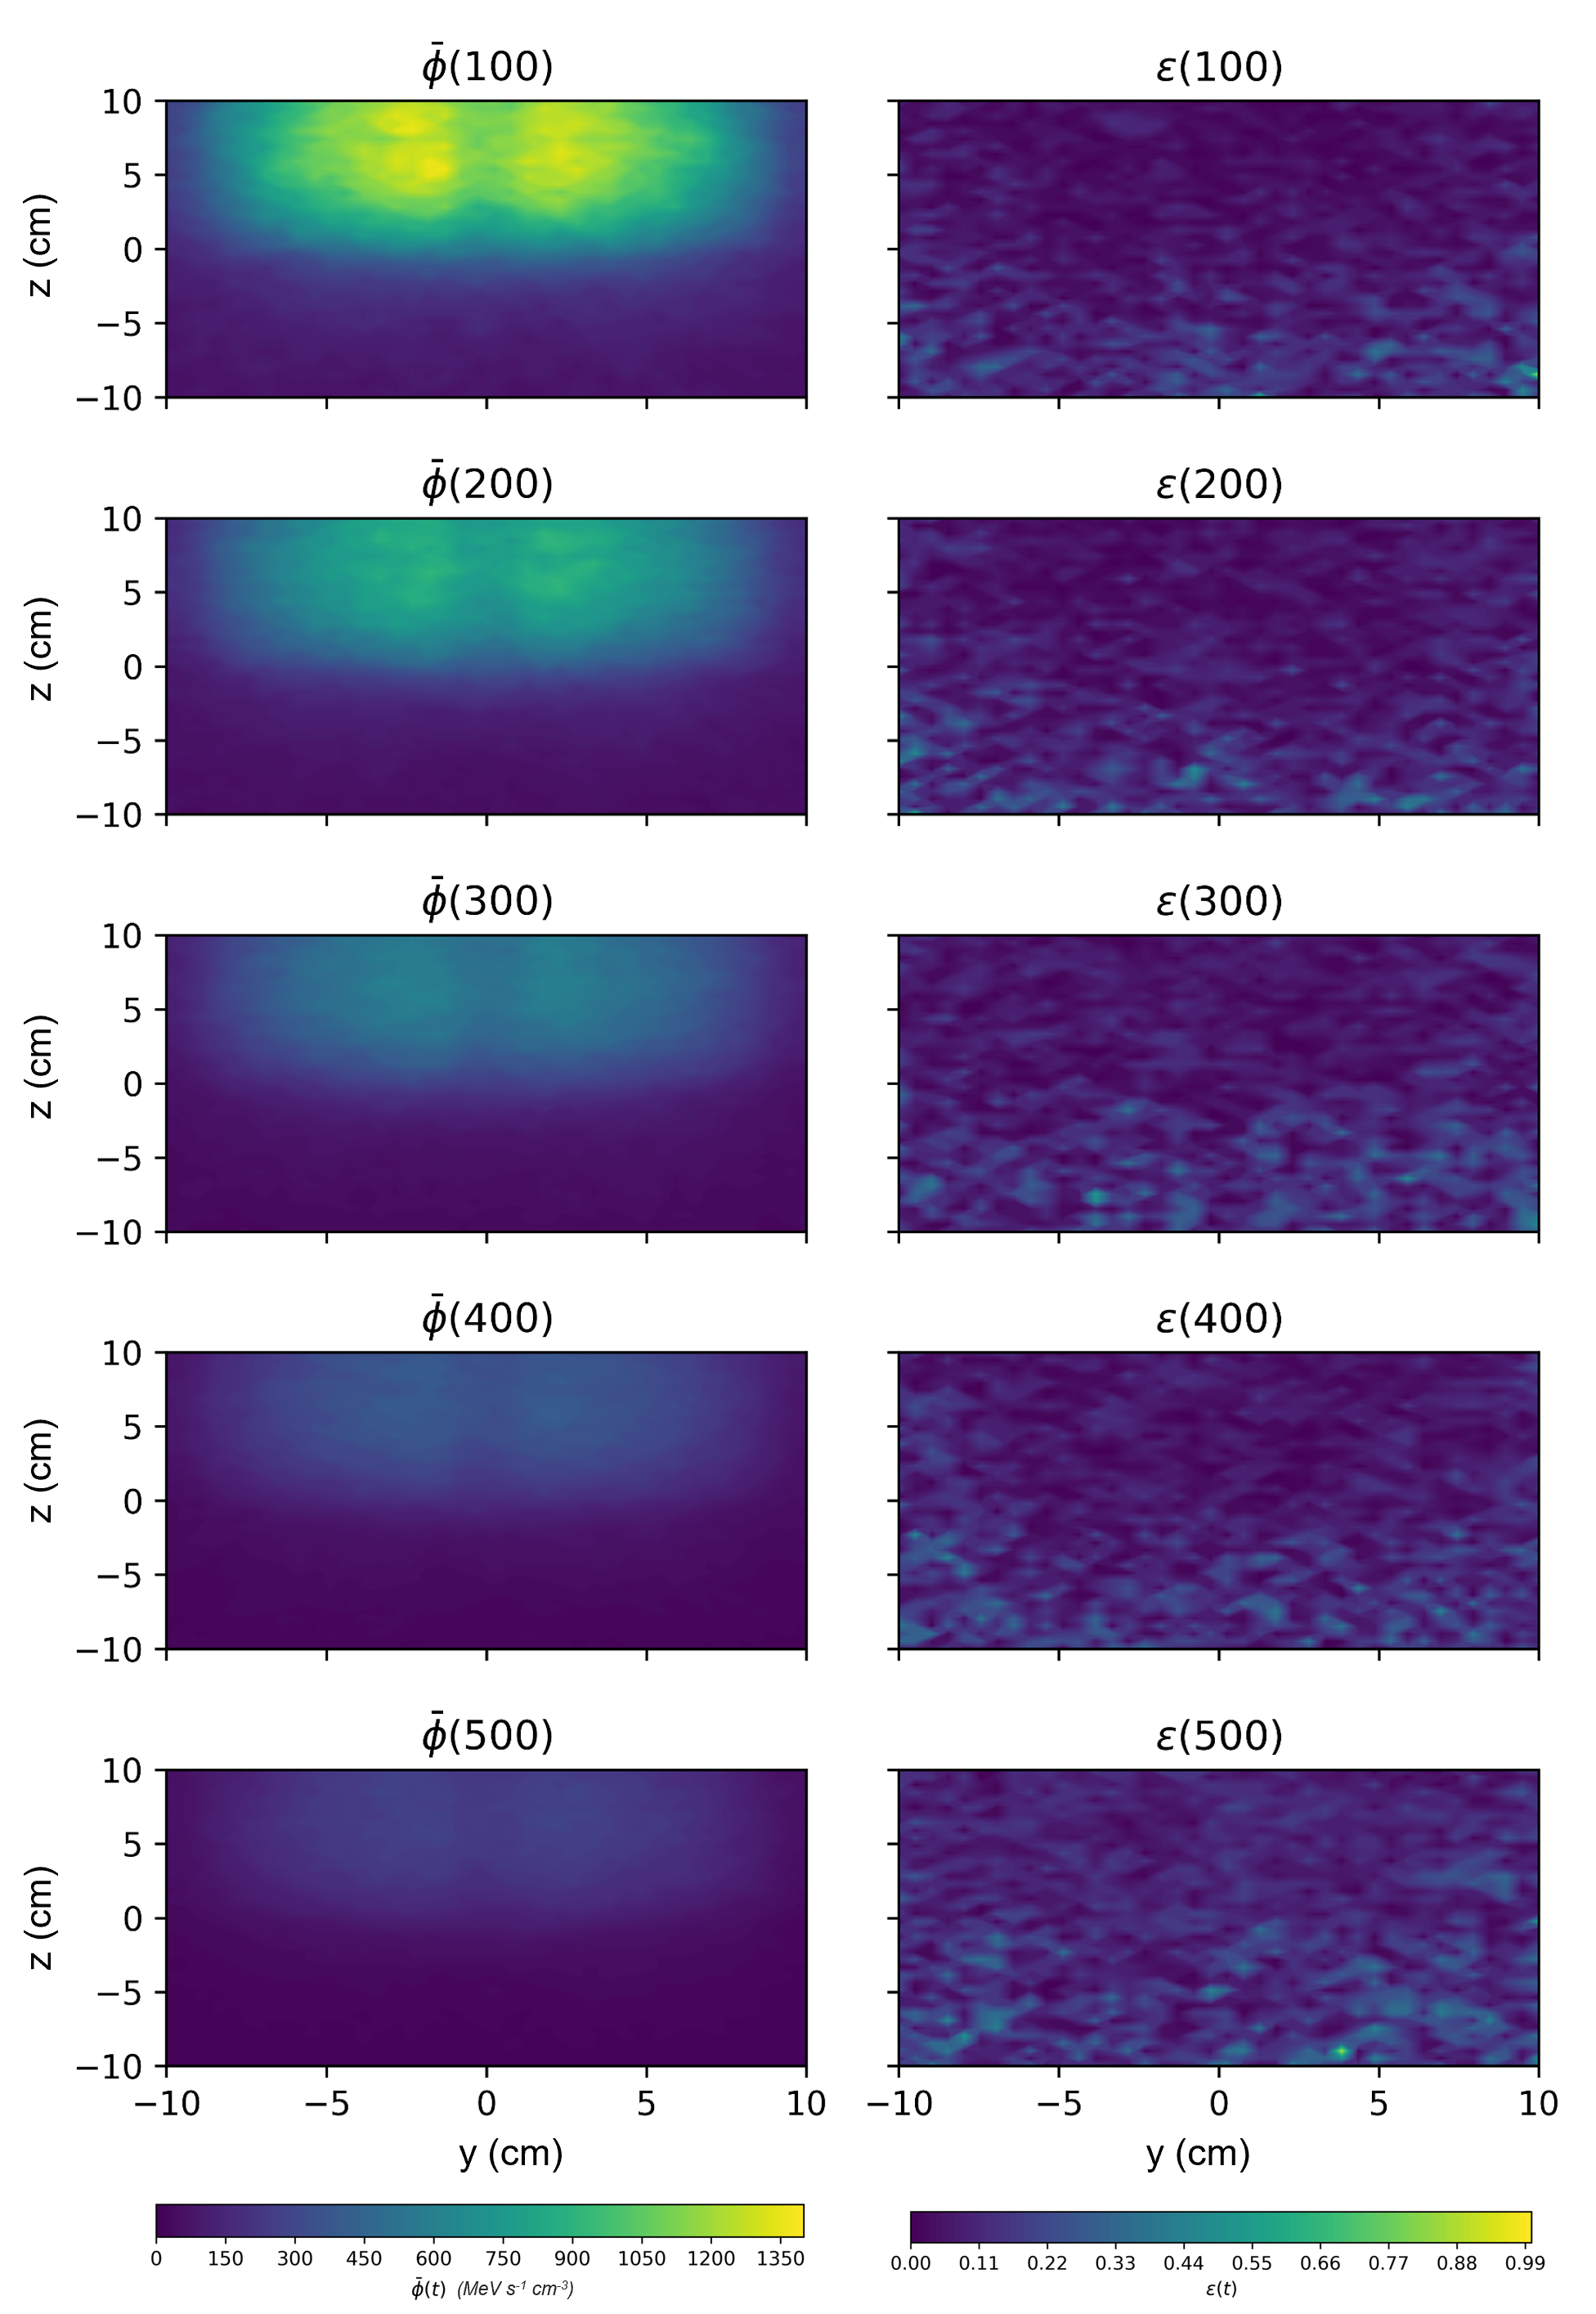
\includegraphics[width=.85\textwidth]{appendix/mcatk_figures/godiva_plot.png}
  \caption{Right: Spatial averaged scalar flux of Godiva IV (HEU-MET-FAST-086) from MCATK. Left: Relative error between solution from standard tracking algorithm and hybrid-delta tracking. Shown through time (every \SI{1e-8}{\s}).}
  \label{fig:godiva_results}
\end{figure}


Figure \ref{fig:godiva_results} at left shows spatial averaged scalar flux ($\bar{\phi}$) of the \num{0.1} to \SI{1.0}{\mega\electronvolt} energy bin on an $y-z$ plane slice at $x=$ \SI{0}{\centi\meter} in a high fidelity version (same simulation but with \num{1e8} particles per time step) of Godiva IV as a fixed source problem. The source in this simulation is an isotropic burst of neutrons at $(0,0,0)$ \unit{\centi\meter} and $t=0.0$ \unit{\s} with an energy of \SI{1}{\mega\electronvolt}.
At right Figure \ref{fig:godiva_results} shows the relative error
\begin{equation}
    \epsilon = \frac{\left|\bar{\phi}_{\Delta} - \bar{\phi}_{\text{Standard}}\right|}{\bar{\phi}_{\Delta}},
\end{equation}
where $\bar{\phi}_{\Delta}$ is the spatial averaged scalar flux solution from the hybrid-delta tracking scheme and $\bar{\phi}_{\text{Standard}}$ is from the standard tracking scheme.
It shows that the relative error in this slice is small between the two methods of tracking.
This further demonstrates that a hybrid-delta tracking scheme is not biasing the results of MCATK's standard surface tracking algorithm in these models. 


\section{CONCLUSIONS \& FUTURE WORK}
Hybrid-delta tracking on a structured mesh improves run time in large and materially complex simulations like the ones we benchmarked: 1.5---1.75$\times$ speed-up for k-eigenvalue and 1.2---1.6$\times$ speed-up for fixed source problems.
We expect further optimizations will improve speed-up for these algorithms.

The solutions found with hybrid-delta tracking match to within three standard deviations of solutions found with MCATK's standard algorithm. 
The advantages of this algorithm over full delta tracking on structured meshes are that track-length estimators may still be used, and that minimal the changes are required to the code as the treatment of the geometry does not change.

Further work is required to verify and validate the hybrid-delta tracking scheme.
For k-eigenvalue problems we will use the criticality validation suite for MCNP \cite{mcnpCriticality} as well as other criticality benchmarks such as the Sub-critical Copper-Reflected $\alpha$-phase Pu (SCR$\alpha$P) experiment \cite{ICSBEP_2020}.
For fixed source solutions we will verify with the analytical AZURV1 \cite{ganapol_homogeneous_2001} benchmark problems. We also plan to study how the algorithm performs as a function of time step size, since small time steps can suffer from poor performance in a similar manner as small cell sizes.

We expect that this work will increase the overall performance of MCATK when delta tracking is appropriately used in problems that warrant it.

\section*{ACKNOWLEDGEMENTS}
Research presented in this article was supported by the Laboratory Directed Research and Development program of Los Alamos National Laboratory under project number 20220084DR.

This work was supported by the Center for Exascale Monte-Carlo Neutron Transport (CEMeNT) a PSAAP-III project funded by the Department of Energy, grant number: DE-NA003967.

The authors would like to R. Arthur Forster for the discussions that inspired this work as well as Theresa Cutler, Travis Smith, and Robert Weldon Jr. for providing benchmark problem input files.

LA-UR-23-24971


\end{document}
